
% \part{Tutorials and Guidelines}

\part{教程和准则}

{\Large \emph{by Till Tantau}}

\bigskip

% \noindent To help you get started with \tikzname, instead of a long installation and configuration section, this manual starts with tutorials. They explain all the basic and some of the more advanced features of the system, without going into all the details. This part also contains some guidelines on how you should proceed when creating graphics using \tikzname.

\noindent 为了帮助您开始使用\tikzname ,而不是冗长的安装和配置部分,本手册从教程开始。 它们解释了系统的所有基本和一些更高级的功能,而没有涉及所有细节。 本部分还包含一些有关使用\tikzname 创建图形时应如何进行操作的准则。

\vskip3cm

\begin{codeexample}[graphic=white,width=0pt]
\tikz \draw[thick,rounded corners=8pt]
  (0,0) -- (0,2) -- (1,3.25) -- (2,2) -- (2,0) -- (0,2) -- (2,2) -- (0,0) -- (2,0);
\end{codeexample}

\clearpage

% Copyright 2009 by Till Tantau
%
% This file may be distributed and/or modified
%
% 1. under the LaTeX Project Public License and/or
% 2. under the GNU Free Documentation License.
%
% See the file doc/generic/pgf/licenses/LICENSE for more details.


% \section{Tutorial: A Picture for Karl's Students}
\section{教程:卡尔学生的图片}

% This tutorial is intended for new users of \tikzname. It does not give an exhaustive account of all the features of \tikzname, just of those that you are likely to use right away. 

本教程适用于\tikzname 的新用户。 它没有详尽介绍\tikzname 的所有功能,只是您可能立即使用的那些功能。

% Karl is a math and chemistry high-school teacher. He used to create the graphics in his worksheets and exams using \LaTeX's |{picture}| environment. While the results were acceptable, creating the graphics often turned out to be a lengthy process. Also, there tended to be problems with lines having slightly wrong angles and circles also seemed to be hard to get right. Naturally, his students could not care less whether the lines had the exact right angles and they find Karl's exams too difficult no matter how nicely they were drawn. But Karl was never entirely satisfied with the result.

卡尔(Karl)是一位数学和化学高中老师。 他曾经使用\LaTeX 的 |{picture}| 环境在练习题和考试中创建图形。 虽然结果是可以接受的,但是创建图形往往是一个漫长的过程。 另外,角度略有错误的直线也容易出现问题,圆也似乎难以正确。 自然,他的学生们并不在乎这些线是否具有正确的直角,并且无论画得多么好,他们都觉得卡尔的考试太难了。 但是卡尔从未对结果完全满意。

% Karl's son, who was even less satisfied with the results (he did not have to take the exams, after all), told Karl that he might wish to try out a new package for creating graphics. A bit confusingly, this package seems to have two names: First, Karl had to download and install a package called \pgfname. Then it turns out that inside this package there is another package called \tikzname, which is supposed to stand for ``\tikzname\ ist \emph{kein} Zeichenprogramm''. Karl finds this all a bit strange and \tikzname\ seems to indicate that the package does not do what he needs. However, having used \textsc{gnu} software for quite some time and ``\textsc{gnu} not being Unix'', there seems to be hope yet. His son assures him that \tikzname's name is intended to warn people that \tikzname\ is not a program that you can use to draw graphics with your mouse or tablet. Rather, it is more like a ``graphics language''. 

卡尔的儿子对这样的结果并不满意(毕竟他不必参加考试),他告诉卡尔,他可能希望尝试一种用于制作图形的新的宏包。 有点令人困惑的是,该宏包似乎有两个名称:首先,卡尔必须下载并安装一个名为\pgfname 的宏包。 然后事实证明,在该程序包中还有另一个名为\tikzname 的宏包,它应该表示``\tikzname\ ist \emph{kein} Zeichenprogramm(\tikzname 不是一个绘图程序)''。  卡尔发现这一切都有些奇怪,\tikzname\ 似乎表明该宏包无法满足他的需要。 但是,使用\textsc{gnu}软件已经有一段时间了,并且``\textsc{gnu}不是Unix'',似乎还有希望。 他的儿子向他保证,\tikzname\ 的名称旨在警告人们,\tikzname\ 不是可用于使用鼠标或平板电脑绘制图形的程序。 相反,它更像是一种``图形语言''。

% \subsection{Problem Statement}
\subsection{问题描述}

% Karl wants to put a graphic on the next worksheet for his students. He is currently teaching his students about sine and cosine. What he would like to have is something that looks like this (ideally):

卡尔希望在下一次练习题中为他的学生添加一张图解。 他目前正在向学生教授正弦和余弦。 他想绘制的图形(理想情况下)如下所示:

%
\noindent
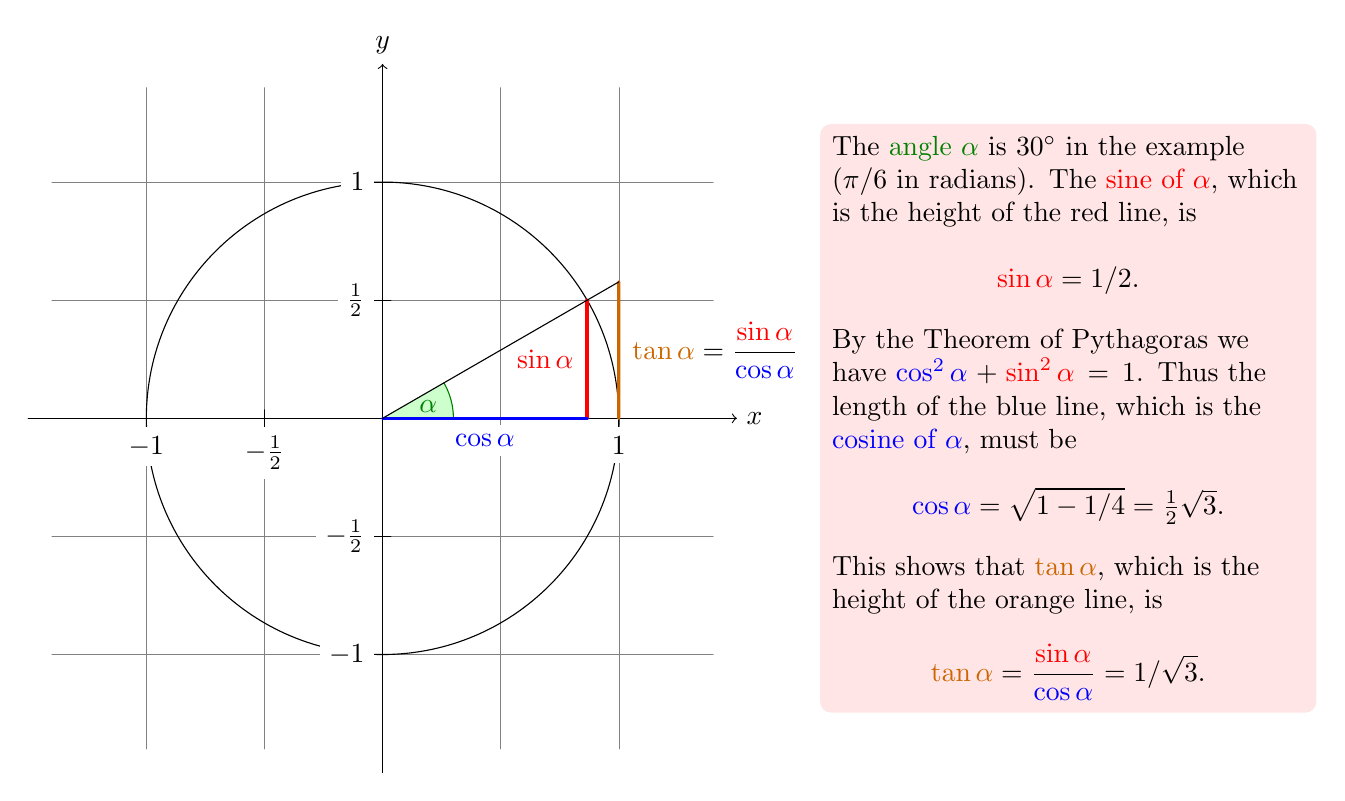
\begin{tikzpicture}
  [scale=3,line cap=round,
   % Styles
   axes/.style=,
   important line/.style={very thick},
   information text/.style={rounded corners,fill=red!10,inner sep=1ex}]

  % Local definitions
  \def\costhirty{0.8660256}

  % Colors
  \colorlet{anglecolor}{green!50!black}
  \colorlet{sincolor}{red}
  \colorlet{tancolor}{orange!80!black}
  \colorlet{coscolor}{blue}

  % The graphic
  \draw[help lines,step=0.5cm] (-1.4,-1.4) grid (1.4,1.4);

  \draw (0,0) circle [radius=1cm];

  \begin{scope}[axes]
    \draw[->] (-1.5,0) -- (1.5,0) node[right] {$x$};
    \draw[->] (0,-1.5) -- (0,1.5) node[above] {$y$};

    \foreach \x/\xtext in {-1, -.5/-\frac{1}{2}, 1}
      \draw[xshift=\x cm] (0pt,1pt) -- (0pt,-1pt) node[below,fill=white] {$\xtext$};

    \foreach \y/\ytext in {-1, -.5/-\frac{1}{2}, .5/\frac{1}{2}, 1}
      \draw[yshift=\y cm] (1pt,0pt) -- (-1pt,0pt) node[left,fill=white] {$\ytext$};
  \end{scope}

  \filldraw[fill=green!20,draw=anglecolor] (0,0) -- (3mm,0pt) arc(0:30:3mm);
  \draw (15:2mm) node[anglecolor] {$\alpha$};

  \draw[important line,sincolor]
    (30:1cm) -- node[left=1pt,fill=white] {$\sin \alpha$} +(0,-.5);

  \draw[important line,coscolor]
    (0,0) -- node[below=2pt,fill=white] {$\cos \alpha$} (\costhirty,0);

  \draw[important line,tancolor] (1,0) --
    node [right=1pt,fill=white]
    {
      $\displaystyle \tan \alpha \color{black}=
      \frac{{\color{sincolor}\sin \alpha}}{\color{coscolor}\cos \alpha}$
    } (intersection of 0,0--30:1cm and 1,0--1,1) coordinate (t);

  \draw (0,0) -- (t);

  \draw[xshift=1.85cm] node [right,text width=6cm,information text]
    {
      The {\color{anglecolor} angle $\alpha$} is $30^\circ$ in the example ($\pi/6$ in radians). The {\color{sincolor}sine of $\alpha$}, which is the height of the red line, is

      % 示例中,{\color{anglecolor}角度$\alpha$}为$30^\circ$(弧度为$\pi/6$)。 {$\alpha$的\color{sincolor}正弦值},即红线的高度,为
      \[
      {\color{sincolor} \sin \alpha} = 1/2.
      \]

      By the Theorem of Pythagoras we have ${\color{coscolor}\cos^2 \alpha} + {\color{sincolor}\sin^2\alpha} =1$. Thus the length of the blue line, which is the {\color{coscolor}cosine of $\alpha$}, must be

      % 根据勾股定理,我们得到${\color{coscolor}\cos^2 \alpha} + {\color{sincolor}\sin^2\alpha} =1$。 因此,蓝线的长度应该是{\color{coscolor} $\alpha$}的余弦
      \[
      {\color{coscolor}\cos\alpha} = \sqrt{1 - 1/4} = \textstyle
      \frac{1}{2} \sqrt 3.
      \]%
      This shows that {\color{tancolor}$\tan \alpha$}, which is the height of the orange line, is
      
      % 这表明{\color{tancolor} $\tan\alpha$},即橙线的高度,为
      \[
      {\color{tancolor}\tan\alpha} = \frac{{\color{sincolor}\sin
          \alpha}}{\color{coscolor}\cos \alpha} = 1/\sqrt 3.
      \]%
    };
\end{tikzpicture}

% \subsection{Setting up the Environment}
\subsection{配置环境}

% In \tikzname, to draw a picture, at the start of the picture you need to tell \TeX\ or \LaTeX\ that you want to start a picture. In \LaTeX\ this is done using the environment |{tikzpicture}|, in plain \TeX\ you just use |\tikzpicture| to start the picture and |\endtikzpicture| to end it. 

在\tikzname 中绘制图片,在图片的开头,您需要告诉\TeX\ 或\LaTeX\ 您要开始绘制图片。在\LaTeX\ 中,这是使用 |{tikzpicture}| 环境完成的,在Plain \TeX\ 中,您只需使用 |\tikzpicture| 开始绘制图片以及使用 |\endtikzpicture| 结束绘制。

% \subsubsection{Setting up the Environment in \LaTeX}
\subsubsection{在\LaTeX 中配置环境}

% Karl, being a \LaTeX\ user, thus sets up his file as follows:

卡尔作为一个\LaTeX\ 用户,他的文件如下:

%
\begin{codeexample}[code only]
\documentclass{article} % say
\usepackage{tikz}
\begin{document}
We are working on
\begin{tikzpicture}
  \draw (-1.5,0) -- (1.5,0);
  \draw (0,-1.5) -- (0,1.5);
\end{tikzpicture}.
\end{document}
\end{codeexample}

% When executed, that is, run via |pdflatex| or via |latex| followed by |dvips|, the resulting will contain something that looks like this:

执行后,即通过运行 |pdflatex| 或通过运行 |latex| 然后运行 |dvips|,结果将包含如下内容:

%
\begin{codeexample}[width=7cm]
We are working on
\begin{tikzpicture}
  \draw (-1.5,0) -- (1.5,0);
  \draw (0,-1.5) -- (0,1.5);
\end{tikzpicture}.
\end{codeexample}

% Admittedly, not quite the whole picture, yet, but we do have the axes established. Well, not quite, but we have the lines that make up the axes drawn. Karl suddenly has a sinking feeling that the picture is still some way off.

诚然,这还不是全部,但我们确实已经确定了坐标轴。 好吧,虽然不完全,但是我们有构成绘制坐标轴的线。 卡尔突然感到那张图解还差得远。

% Let's have a more detailed look at the code. First, the package |tikz| is loaded. This package is a so-called ``frontend'' to the basic \pgfname\ system. The basic layer, which is also described in this manual, is somewhat more, well, basic and thus harder to use. The frontend makes things easier by providing a simpler syntax. 

让我们更详细地看一下代码。 首先,包 |tikz| 已加载。该软件包是基本\pgfname\ 系统的所谓的``前端''。本手册中也介绍了基础层,它更基础一些,因此也更难使用。前端通过提供更简单的语法使事情变得更容易。

% Inside the environment there are two |\draw| commands. They mean: ``The path, which is specified following the command up to the semicolon, should be drawn.'' The first path is specified as |(-1.5,0) -- (0,1.5)|, which means ``a straight line from the point at position $(-1.5,0)$ to the point at position $(0,1.5)$''. Here, the positions are specified within a special coordinate system in which, initially, one unit is 1cm.

在环境内部有两个 |\draw| 命令。它们的意思是:“应该绘制从命令到分号为止指定的路径。”第一个路径指定为 |(-1.5,0) -- (0,1.5)|,表示`“从位置$(-1.5,0)$到位置$(0,1.5)$的直线”。在此,位置是在特殊坐标系中指定的,初始条件下,一个单位为1厘米。

% Karl is quite pleased to note that the environment automatically reserves enough space to encompass the picture. 

卡尔非常高兴地注意到环境会自动保留足够的空间来容纳图片。

% \subsubsection{Setting up the Environment in Plain \TeX}
\subsubsection{在Plain \TeX 中配置环境}

% Karl's wife Gerda, who also happens to be a math teacher, is not a \LaTeX\ user, but uses plain \TeX\ since she prefers to do things ``the old way''. She can also use \tikzname. Instead of |\usepackage{tikz}| she has to write |\input tikz.tex| and instead of |\begin{tikzpicture}| she writes |\tikzpicture| and instead of |\end{tikzpicture}| she writes |\endtikzpicture|.

卡尔的妻子格达(Gerda)恰好也是一名数学老师,她不是\LaTeX\ 用户,而使用Plain \TeX\ ,因为她更喜欢以``旧方式''做事。她还可以使用\tikzname 。她必须使用 |\inputtikz.tex| 代替 |\usepackage{tikz}|,使用 |\tikzpicture| 代替 |\begin{tikzpicture}| 以及使用 |\endtikzpicture| 代替 |\end{tikzpicture}|。

% Thus, she would use:

因此,她将使用:

%
\begin{codeexample}[code only]
%% Plain TeX file
\input tikz.tex
\baselineskip=12pt
\hsize=6.3truein
\vsize=8.7truein
We are working on
\tikzpicture
  \draw (-1.5,0) -- (1.5,0);
  \draw (0,-1.5) -- (0,1.5);
\endtikzpicture.
\bye
\end{codeexample}

% Gerda can typeset this file using either |pdftex| or |tex| together with |dvips|. \tikzname\ will automatically discern which driver she is using. If she wishes to use |dvipdfm| together with |tex|, she either needs to modify the file |pgf.cfg| or can write |\def\pgfsysdriver{pgfsys-dvipdfm.def}| somewhere \emph{before} she inputs |tikz.tex| or |pgf.tex|.

格达可以使用 |pdftex| 或者 |tex| 和 |dvips| 来排版这个文件。\tikzname\ 将自动识别她正在使用哪个驱动程序。如果她希望同时使用 |dvipdfm| 和 |tex|,那么她需要修改文件 |pgf.cfg| 或可以在她输入 |tikz.tex| 或 |pgf.tex| 的位置\emph{之前}添加 |\def\pgfsysdriver{pgfsys-dvipdfm.def}|。


% \subsubsection{Setting up the Environment in Con\TeX t}
\subsubsection{在 Con\TeX t 中配置环境}

% Karl's uncle Hans uses Con\TeX t. Like Gerda, Hans can also use \tikzname. Instead of |\usepackage{tikz}| he says |\usemodule[tikz]|. Instead of |\begin{tikzpicture}| he writes |\starttikzpicture| and  instead of |\end{tikzpicture}| he writes |\stoptikzpicture|.

卡尔的叔叔汉森(Hans)使用Con\TeX t。与格达一样,汉森也可以使用\tikzname 。他将使用 |\usemodule[tikz]| 代替 |\usepackage{tikz}|。使用 |\starttikzpicture| 代替 |\begin{tikzpicture}|,使用 |\stoptikzpicture| 代替 |\end{tikzpicture}|。

% His version of the example looks like this:

他的示例版本如下所示:

%
\begin{codeexample}[code only]
%% ConTeXt file
\usemodule[tikz]

\starttext
  We are working on
  \starttikzpicture
    \draw (-1.5,0) -- (1.5,0);
    \draw (0,-1.5) -- (0,1.5);
  \stoptikzpicture.
\stoptext
\end{codeexample}

% Hans will now typeset this file in the usual way using |texexec| or |context|.

汉森现在将使用 |texexec| 或 |context|,并且以通常的方式排版此文件。


% \subsection{Straight Path Construction}
\subsection{直线路径的创建}

% The basic building block of all pictures in \tikzname\ is the path. A \emph{path} is a series of straight lines and curves that are connected (that is not the whole picture, but let us ignore the complications for the moment). You start a path by specifying the coordinates of the start position as a point in round brackets, as in |(0,0)|. This is followed by a series of ``path extension operations''. The simplest is |--|, which we used already. It must be followed by another coordinate and it extends the path in a straight line to this new position. For example, if we were to turn the two paths of the axes into one path, the following would result:

\tikzname\ 中所有图片的基本构造块是路径。一个\emph{路径}是一系列相连的直线和曲线(这不是全部,但让我们暂时忽略复杂性)。通过将起始位置的坐标指定为方括号中的点来启动路径,如 |(0,0)| 中所示。接下来是一系列“路径扩展操作”。最简单的是 |--|,我们已经用过了。它必须跟随着另一个坐标,它将路径以直线延伸到这个新位置。例如,如果我们将坐标轴的两条路径变换为一条路径,会得到如下结果:

%
\begin{codeexample}[]
\tikz \draw (-1.5,0) -- (1.5,0) -- (0,-1.5) -- (0,1.5);
\end{codeexample}

% Karl is a bit confused by the fact that there is no |{tikzpicture}| environment, here. Instead, the little command |\tikz| is used. This command either takes one argument (starting with an opening brace as in |\tikz{\draw (0,0) -- (1.5,0)}|, which yields \tikz{\draw (0,0) --(1.5,0);}) or collects everything up to the next semicolon and puts it inside a |{tikzpicture}| environment. As a rule of thumb, all \tikzname\ graphic drawing commands must occur as an argument of |\tikz| or inside a |{tikzpicture}| environment. Fortunately, the command |\draw| will only be defined inside this environment, so there is little chance that you will accidentally do something wrong here.

卡尔对这里没有 |{tikzpicture}| 环境这一事实感到有点困惑。相反,使用小命令 | \tikz|。这个命令要么接受一个参数(以 |\tikz{\draw(0,0)--(1.5,0)}| 中的括号开始,这会产生\tikz{\draw(0,0)--(1.5,0);}),要么收集所有内容,直到下一个分号,并将其放到 |{tikzpicture}| 环境中。根据经验,所有\tikzname\ 图形绘制命令都必须作为 |\tikz| 的参数出现,或者出现在 |{tikzpicture}| 环境中。幸运的是,命令 |\draw| 将只在这个环境中定义,因此您不太可能在这里意外地出错。


% \subsection{Curved Path Construction}
\subsection{曲线路径的创建}

% The next thing Karl wants to do is to draw the circle. For this, straight lines obviously will not do. Instead, we need some way to draw curves. For this, \tikzname\ provides a special syntax. One or two ``control points'' are needed. The math behind them is not quite trivial, but here is the basic idea: Suppose you are at point $x$ and the first control point is $y$. Then the curve will start ``going in the direction of~$y$ at~$x$'', that is, the tangent of the curve at $x$ will point toward~$y$. Next, suppose the curve should end at $z$ and the second support point is $w$. Then the curve will, indeed, end at $z$ and the tangent of the curve at point $z$ will go through $w$.

卡尔想做的下一件事是画圆。对于这个问题,直线显然是不行的。相反,我们需要一些绘制曲线的方法。为此,\tikzname\ 提供了特殊的语法。需要一两个“控制点”。它们背后的数学原理并不简单,但基本的思想是:假设您在点$x$,第一个控制点是$y$。然后曲线将开始朝着~$y$在~$x$的方向,也就是说,曲线在$x$处的切线将指向~$y$。接下来,假设曲线应该结束于$z$,第二个控制点是$w$。曲线会在$z$点结束曲线在$z$点的切线会经过$w$点。

% Here is an example (the control points have been added for clarity):

这是一个示例(为清楚起见添加了控制点):

%
\begin{codeexample}[]
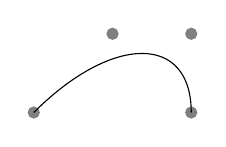
\begin{tikzpicture}
  \filldraw [gray] (0,0) circle [radius=2pt]
                   (1,1) circle [radius=2pt]
                   (2,1) circle [radius=2pt]
                   (2,0) circle [radius=2pt];
  \draw (0,0) .. controls (1,1) and (2,1) .. (2,0);
\end{tikzpicture}
\end{codeexample}

% The general syntax for extending a path in a ``curved'' way is |.. controls| \meta{first control point} |and| \meta{second control point} |..| \meta{end point}. You can leave out the |and| \meta{second control point}, which causes the first one to be used twice.

% 以“弯曲”方式扩展路径的一般语法是| ..控件|  \ meta {第一个控制点} |和|  \ meta {第二控制点} | .. |  \ meta {end point}。 您可以忽略|和|  \ meta {第二控制点},这会使第一个控制点使用两次。

以“弯曲”方式扩展路径的一般语法是 |.. controls| \meta{第一个控制点} |and| \meta{第二个控制点} |..|。您可以省略 |and| \meta{第二个控制点},这将使第一个控制点被使用两次。

% So, Karl can now add the first half circle to the picture:

因此,卡尔现在可以将前半圆添加到图片中:

%
\begin{codeexample}[]
\begin{tikzpicture}
  \draw (-1.5,0) -- (1.5,0);
  \draw (0,-1.5) -- (0,1.5);
  \draw (-1,0) .. controls (-1,0.555) and (-0.555,1) .. (0,1)
               .. controls (0.555,1) and (1,0.555) .. (1,0);
\end{tikzpicture}
\end{codeexample}

% Karl is happy with the result, but finds specifying circles in this way to be extremely awkward. Fortunately, there is a much simpler way.

卡尔对结果感到满意,但是发现以这种方式指定圆非常尴尬。 幸运的是,有一种更简单的方法。


% \subsection{Circle Path Construction}
\subsection{圆路径的创建}

% In order to draw a circle, the path construction operation |circle| can be used. This operation is followed by a radius in brackets as in the following example: (Note that the previous position is used as the \emph{center} of the circle.)

为了画一个圆,可以使用路径构建运算符 |circ|。 此运算符后跟方括号中的半径,如以下示例所示:(请注意,运算符之前的位置用作圆的\emph{圆心}。)

%
\begin{codeexample}[]
\tikz \draw (0,0) circle [radius=10pt];
\end{codeexample}

% You can also append an ellipse to the path using the |ellipse| operation. Instead of a single radius you can specify two of them:

您也可以使用 |ellipse| 操作添加椭圆路径。 您可以指定两个,而不是单个半径:

%
\begin{codeexample}[]
\tikz \draw (0,0) ellipse [x radius=20pt, y radius=10pt];
\end{codeexample}

% To draw an ellipse whose axes are not horizontal and vertical, but point in an arbitrary direction (a ``turned ellipse'' like \tikz \draw[rotate=30] (0,0) ellipse [x radius=6pt, y radius=3pt];) you can use transformations, which are explained later. The code for the little ellipse is |\tikz \draw[rotate=30] (0,0) ellipse [x radius=6pt, y radius=3pt];|, by the way.

要绘制的轴线不是水平和竖直的,而是指向任意方向的椭圆(一个像这样旋转后的椭圆\tikz \draw[rotate=30] (0,0) ellipse [x radius=6pt, y radius=3pt];),您可以使用旋转,稍后将对此进行解释。顺便提一下,小椭圆的代码是 |\tikz \draw[rotate=30] (0,0) ellipse [x radius=6pt, y radius=3pt];|。

% So, returning to Karl's problem, he can write |\draw (0,0) circle [radius=1cm];| to draw the circle:

那么,回到卡尔的问题,他可以写 |\draw (0,0) circle [radius=1cm];| 画圆:

%
\begin{codeexample}[]
\begin{tikzpicture}
  \draw (-1.5,0) -- (1.5,0);
  \draw (0,-1.5) -- (0,1.5);
  \draw (0,0) circle [radius=1cm];
\end{tikzpicture}
\end{codeexample}

% At this point, Karl is a bit alarmed that the circle is so small when he wants the final picture to be much bigger. He is pleased to learn that \tikzname\ has powerful transformation options and scaling everything by a factor of three is very easy. But let us leave the size as it is for the moment to save some space.

在这一点上,卡尔有点惊慌,圆是如此之小,他想要最后的图片大得多。他很高兴地了解到\tikzname\ 具有强大的变换选项,并且很容易将所有内容放大到原来的三倍。但是为了节省一些空间,让我们暂时保持大小不变。


% \subsection{Rectangle Path Construction}
\subsection{矩形路径的创建}

% The next things we would like to have is the grid in the background. There are several ways to produce it. For example, one might draw lots of rectangles. Since rectangles are so common, there is a special syntax for them: To add a rectangle to the current path, use the |rectangle| path construction operation. This operation should be followed by another coordinate and will append a rectangle to the path such that the previous coordinate and the next coordinates are corners of the rectangle. So, let us add two rectangles to the picture:

接下来我们想要的是背景中的网格。有几种方法可以产生它。例如,有人可能会画很多矩形。由于矩形非常常见,因此它们有一种特殊的语法:要向当前路径添加矩形,我们使用 |rectangle| 路径构造操作。该操作之后应该跟着另一个坐标,并将一个矩形添加到路径中,使前一个坐标和下一个坐标都是矩形的角点。所以,我们添加两个矩形的图片:

%
\begin{codeexample}[]
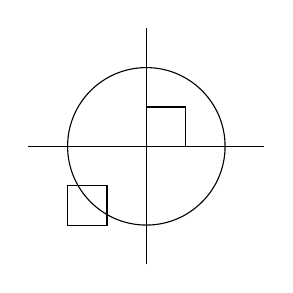
\begin{tikzpicture}
  \draw (-1.5,0) -- (1.5,0);
  \draw (0,-1.5) -- (0,1.5);
  \draw (0,0) circle [radius=1cm];
  \draw (0,0) rectangle (0.5,0.5);
  \draw (-0.5,-0.5) rectangle (-1,-1);
\end{tikzpicture}
\end{codeexample}

% While this may be nice in other situations, this is not really leading anywhere with Karl's problem: First, we would need an awful lot of these rectangles and then there is the border that is not ``closed''.

虽然这在其他情况下可能很好,但这并没有真正解决卡尔的问题:首先,我们需要大量的矩形,然后边界没有“封闭”。

% So, Karl is about to resort to simply drawing four vertical and four horizontal lines using the nice |\draw| command, when he learns that there is a |grid| path construction operation. 

因此,当卡尔得知有一个 |grid| 路径构造操作时,他打算使用漂亮的 |\draw| 命令简单地绘制四条垂直和四条水平线。

% \subsection{Grid Path Construction}
\subsection{网格路径的创建}

% The |grid| path operation adds a grid to the current path. It will add lines making up a grid that fills the rectangle whose one corner is the current point and whose other corner is the point following the |grid| operation. For example, the code |\tikz \draw[step=2pt] (0,0) grid (10pt,10pt);| produces \tikz \draw[step=2pt] (0,0) grid (10pt,10pt);. Note how the optional argument for |\draw| can be used to specify a grid width (there are also |xstep| and |ystep| to define the steppings independently). As Karl will learn soon, there are \emph{lots} of things that can be influenced using such options.

|grid| 路径操作向当前路径添加一个网格。它将添加组成网格的线,填充矩形,矩形的一个角点是当前点,另一个角点是紧跟 |grid| 操作的点。例如,代码 |\tikz \draw[step=2pt] (0,0) grid (10pt,10pt);| 生成 \tikz \draw[step=2pt] (0,0) grid (10pt,10pt);。请注意,可以使用 |\draw| 的可选参数来指定网格宽度(还有 |xstep| 和 |ystep| 来分别定义步长)。卡尔很快就会了解到,使用这些选项可以影响到\emph{很多}事情。

% For Karl, the following code could be used:

对于卡尔来说,可以使用以下代码:

%
\begin{codeexample}[]
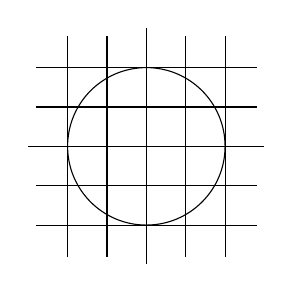
\begin{tikzpicture}
  \draw (-1.5,0) -- (1.5,0);
  \draw (0,-1.5) -- (0,1.5);
  \draw (0,0) circle [radius=1cm];
  \draw[step=.5cm] (-1.4,-1.4) grid (1.4,1.4);
\end{tikzpicture}
\end{codeexample}

% Having another look at the desired picture, Karl notices that it would be nice for the grid to be more subdued. (His son told him that grids tend to be distracting if they are not subdued.) To subdue the grid, Karl adds two more options to the |\draw| command that draws the grid. First, he uses the color |gray| for the grid lines. Second, he reduces the line width to |very thin|. Finally, he swaps the ordering of the commands so that the grid is drawn first and everything else on top.

再次查看所需的图片后,卡尔注意到,使网格的颜色更浅一点会很好。(他的儿子告诉他,如果不使网格的颜色变浅,网格往往会分散注意力。)为了使网格的颜色变浅,卡尔在 |\draw| 命令中添加了两个选项。首先,他使用 |gray| 颜色表示网格线。 其次,他将线宽减小到 |very thin|。 最后,他交换命令的顺序,以便首先绘制网格,然后再绘制其他所有内容。

%
\begin{codeexample}[]
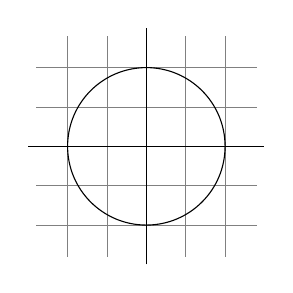
\begin{tikzpicture}
  \draw[step=.5cm,gray,very thin] (-1.4,-1.4) grid (1.4,1.4);
  \draw (-1.5,0) -- (1.5,0);
  \draw (0,-1.5) -- (0,1.5);
  \draw (0,0) circle [radius=1cm];
\end{tikzpicture}
\end{codeexample}


% \subsection{Adding a Touch of  Style}
\subsection{增加一点风格}

% Instead of the options |gray,very thin| Karl could also have said |help lines|. \emph{Styles} are predefined sets of options that can be used to organize how a graphic is drawn. By saying |help lines| you say ``use the style that I (or someone else) has set for drawing help lines''. If Karl decides, at some later point, that grids should be drawn, say, using the color |blue!50| instead of |gray|, he could provide the following option somewhere:

除了使用选项 |gray,very thin|,卡尔也可以声明 |help lines|。 \emph{Styles}是预定义的选项集,可用于组织图形的绘制方式。 通过声明 |help lines| 相当于您说“使用我(或其他人)设置的样式来绘制辅助线”。 如果卡尔在以后的某个时刻决定应该绘制网格,例如使用 |blue!50| 颜色代替 |gray|,他可以在某处提供以下选项:

%
\begin{codeexample}[code only]
help lines/.style={color=blue!50,very thin}
\end{codeexample}
%
%The effect of this ``style setter'' is that in the current scope or environment the |help lines| option has the same effect as |color=blue!50,very thin|.

这种``样式设置器''的作用是,在当前分组或环境中 |help lines| 选项与 |color=blue!50,very thin| 的效果相同。

% Using styles makes your graphics code more flexible. You can change the way things look easily in a consistent manner. Normally, styles are defined at the beginning of a picture. However, you may sometimes wish to define a style globally, so that all pictures of your document can use this style. Then you can easily change the way all graphics look by changing this one style. In this situation you can use the |\tikzset| command at the beginning of the document as in

使用样式可使您的图形代码更加灵活。 您可以以一致的方式更改事物看起来的方式。 通常,样式是在图片的开头定义的。 但是,有时您可能希望全局定义样式,以便文档的所有图片都可以使用此样式。 然后,您可以通过更改一种样式轻松更改所有图形的外观。 在这种情况下,您可以在文档开头使用 |\tikzset| 命令,如

%
\begin{codeexample}[code only]
\tikzset{help lines/.style=very thin}
\end{codeexample}

% To build a hierarchy of styles you can have one style use another. So in order to define a style |Karl's grid| that is based on the |grid| style Karl could say

要建立样式的层级结构,您可以让一种样式使用另一种样式。 因此,为了定义基于 |grid| 风格的样式 |Karl's grid| 卡尔可以这样声明

%
\begin{codeexample}[code only]
\tikzset{Karl's grid/.style={help lines,color=blue!50}}
...
\draw[Karl's grid] (0,0) grid (5,5);
\end{codeexample}

% Styles are made even more powerful by parametrization. This means that, like other options, styles can also be used with a parameter. For instance, Karl could parameterize his grid so that, by default, it is blue, but he could also use another color.

通过参数化,样式变得更加强大。 这意味着,与其他选项一样,样式也可以与参数一起使用。 例如,卡尔可以对网格进行参数化,以便默认情况下为蓝色,但是他也可以使用其他颜色。

%
\begin{codeexample}[code only]
\begin{tikzpicture}
  [Karl's grid/.style  ={help lines,color=#1!50},
   Karl's grid/.default=blue]

  \draw[Karl's grid]     (0,0) grid (1.5,2);
  \draw[Karl's grid=red] (2,0) grid (3.5,2);
\end{tikzpicture}
\end{codeexample}

% In this example, the definition of the style |Karl's grid| is given as an  optional argument to the |{tikzpicture}| environment. Additional styles for other  elements would follow after a comma. With many styles in effect, the optional  argument of the environment may easily happen to be longer than the actual contents.

在此示例中,样式 |Karl's grid| 的定义用作 |{tikzpicture}| 环境的可选参数。 其他元素的附加样式将紧跟在逗号之后。 在使用多种样式的情况下,环境的可选参数可能很容易长于实际内容。

% \subsection{Drawing Options}
\subsection{绘图选项}

% Karl wonders what other options there are that influence how a path is drawn. He saw already that the |color=|\meta{color} option can be used to set the line's color. The option |draw=|\meta{color} does nearly the same, only it sets the color for the lines only and a different color can be used for filling (Karl will need this when he fills the arc for the angle). 

卡尔想知道还有什么其他选项可以影响路径的绘制。他已经看到可以使用 |color=| \meta{color} 选项来设置线条的颜色。选项 |draw=| \meta{color} 做的几乎是一样的,只是它只设置了线条的颜色,可以使用不同的颜色填充(卡尔填充圆弧的角度会用到这个选项)。

% He saw that the style |very thin| yields very thin lines. Karl is not really surprised by this and neither is he surprised to learn that |thin| yields thin lines,  |thick| yields thick lines, |very thick| yields very thick lines, |ultra thick| yields really, really thick lines and |ultra thin| yields lines that are so thin that low-resolution printers and displays will have trouble showing them. He wonders what gives lines of ``normal'' thickness. It turns out that |thin| is the correct choice, since it gives the same thickness as \TeX's |\hrule| command. Nevertheless, Karl would like to know whether there is anything ``in the middle'' between |thin| and |thick|. There is: |semithick|.

他看到样式 |very thin| 产生非常细的线。 卡尔对此并不感到惊讶,也不会惊讶于 |thin| 产生细线,|thick| 产生的粗线,|very thick| 产生非常粗的线,|ultra thick| 产生非常非常粗的线以及 |ultra thin| 产生非常非常细的线,以至于低分辨率的打印机和显示器将很难显示它们。 他想知道是什么使线条具有``正常''的宽度。 事实证明 |thin| 是正确的选择,因为它的厚度与\TeX 的 |\hrule| 命令相同。 但是,卡尔想知道 |thin| 和 |thick| 之间是否有“中间”的宽度。有:|semithick|。

% Another useful thing one can do with lines is to dash or dot them. For this, the two styles |dashed| and |dotted| can be used, yielding \tikz[baseline] \draw[dashed] (0,.5ex) -- ++(2em,0pt); and \tikz[baseline] \draw[dotted] (0,.5ex) -- ++(2em,0pt);. Both options also exist in a loose and a dense version, called |loosely dashed|, |densely dashed|, |loosely dotted|, and |densely dotted|. If he really, really  needs to, Karl can also define much more complex dashing patterns with the |dash pattern| option, but his son insists that dashing is to be used with utmost care and mostly distracts. Karl's son claims that complicated dashing patterns are evil. Karl's students do not care about dashing patterns.

对线条的另一种有用的处理是虚线或点线。为此,可以使用 |dashed| 和 |dotted| 两种样式,产生\tikz[baseline] \draw[dashed] (0,.5ex) -- ++(2em,0pt);和\tikz[baseline] \draw[dotted] (0,.5ex) -- ++(2em,0pt);。这两个选项也存在松散和密集的版本,称为 |loosely dashed|,|densely dashed|,|loosely dotted|,|densely dotted|。如果他真的真的需要,卡尔也可以使用 |dash pattern| 选项定义更复杂的虚线样式,但他的儿子坚持认为,在使用时要格外小心,而且大多会分散注意力。卡尔的儿子声称复杂的虚线图案是邪恶的。卡尔的学生不关心虚线的样式。


% \subsection{Arc Path Construction}
\subsection{弧线路径的创建}

% Our next obstacle is to draw the arc for the angle. For this, the |arc| path construction operation is useful, which draws part of a circle or ellipse. This |arc| operation is followed by options in brackets that specify the arc. An example would be |arc[start angle=10, end angle=80, radius=10pt]|, which means exactly what it says. Karl obviously needs an arc from $0^\circ$ to $30^\circ$. The radius should be something relatively small, perhaps around one third of the circle's radius. When one uses the arc path construction operation, the specified arc will be added with its starting point at the current position. So, we first have to ``get there''.

我们的下一个障碍是绘制该角度的弧线。 为此,|arc| 路径构造操作非常有用,它可以绘制一部分圆或椭圆。 |arc| 操作之后的括号指定圆弧的选项。 一个示例是 |arc [start angle=10, end angle=80, radius=10pt]|,其含义就像它说的那样。 卡尔显然需要从$0^\circ$到$30^\circ$的弧线。 半径应相对较小,可能约为圆半径的三分之一。 当使用弧形路径构造操作时,指定的弧形将以其起始点添加到当前位置。 因此,我们首先必须``到达那里''。

%
\begin{codeexample}[]
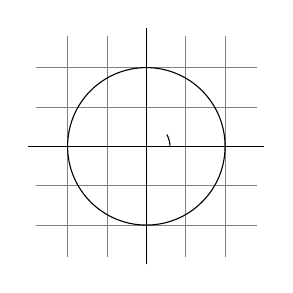
\begin{tikzpicture}
  \draw[step=.5cm,gray,very thin] (-1.4,-1.4) grid (1.4,1.4);
  \draw (-1.5,0) -- (1.5,0);
  \draw (0,-1.5) -- (0,1.5);
  \draw (0,0) circle [radius=1cm];
  \draw (3mm,0mm) arc [start angle=0, end angle=30, radius=3mm];
\end{tikzpicture}
\end{codeexample}

% Karl thinks this is really a bit small and he cannot continue unless he learns how to do scaling. For this, he can add the |[scale=3]| option. He could add this option to each |\draw| command, but that would be awkward. Instead, he adds it to the whole environment, which causes this option to apply to everything within.

卡尔认为这确实有点小,除非学会了缩放方法,否则他无法继续。 为此,他可以添加 \verb|[scale=3]| 选项。 他可以将此选项添加到每个 |\draw| 命令中,但那样做非常麻烦。相反,他将其添加到整个环境中,这使得该选项应用于其中的所有内容。

%
\begin{codeexample}[]
\begin{tikzpicture}[scale=3]
  \draw[step=.5cm,gray,very thin] (-1.4,-1.4) grid (1.4,1.4);
  \draw (-1.5,0) -- (1.5,0);
  \draw (0,-1.5) -- (0,1.5);
  \draw (0,0) circle [radius=1cm];
  \draw (3mm,0mm) arc [start angle=0, end angle=30, radius=3mm];
\end{tikzpicture}
\end{codeexample}

% As for circles, you can specify ``two'' radii in order to get an elliptical arc.

对于圆而言,您可以指定``两个''半径以获得椭圆弧。

%
\begin{codeexample}[]
  \tikz \draw (0,0)
    arc [start angle=0, end angle=315,
         x radius=1.75cm, y radius=1cm];
\end{codeexample}


% \subsection{Clipping a Path}
\subsection{剪切路径}

% In order to save space in this manual, it would be nice to clip Karl's graphics a bit so that we can focus on the ``interesting'' parts. Clipping is pretty easy in \tikzname. You can use the |\clip| command to clip all subsequent drawing. It works like |\draw|, only it does not draw anything, but uses the given path to clip everything subsequently.

为了节省空间,最好裁剪一下卡尔的图形,以便我们专注于“有趣的”部分。 \tikzname 中的剪切非常容易。 您可以使用 |\clip| 命令剪切所有后续图形。 它的工作方式类似于 |\draw|,只是它不绘制任何内容,而是使用给定的路径剪切所有的图形。

%
\begin{codeexample}[]
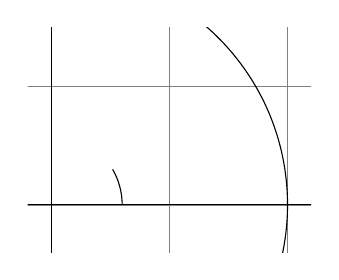
\begin{tikzpicture}[scale=3]
  \clip (-0.1,-0.2) rectangle (1.1,0.75);
  \draw[step=.5cm,gray,very thin] (-1.4,-1.4) grid (1.4,1.4);
  \draw (-1.5,0) -- (1.5,0);
  \draw (0,-1.5) -- (0,1.5);
  \draw (0,0) circle [radius=1cm];
  \draw (3mm,0mm) arc [start angle=0, end angle=30, radius=3mm];
\end{tikzpicture}
\end{codeexample}

% You can also do both at the same time: Draw \emph{and} clip a path. For this, use the |\draw| command and add the |clip| option. (This is not the whole picture: You can also use the |\clip| command and add the |draw| option. Well, that is also not the whole picture: In reality, |\draw| is just a shorthand for |\path[draw]| and |\clip| is a shorthand for |\path[clip]| and you could also say |\path[draw,clip]|.) Here is an example:

你也可以同时做这两件事:绘制\emph{和}剪切一个路径。为此,使用 |\draw| 命令并添加 |clip| 选项。(这并不是全部:您还可以使用 |\clip| 命令并添加 |draw| 选项。实际上,|\draw| 只是 |\path[draw]| 的简写而 |\clip| 是 |\path[clip]| 的简写,而且你也可以这样使用 |\path[draw,clip]|。下面是一个例子:

%
\begin{codeexample}[]
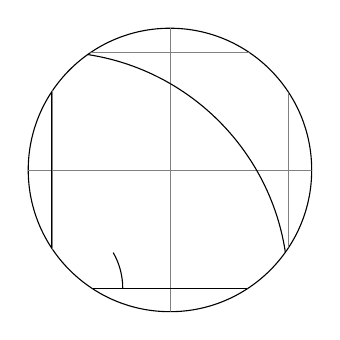
\begin{tikzpicture}[scale=3]
  \clip[draw] (0.5,0.5) circle (.6cm);
  \draw[step=.5cm,gray,very thin] (-1.4,-1.4) grid (1.4,1.4);
  \draw (-1.5,0) -- (1.5,0);
  \draw (0,-1.5) -- (0,1.5);
  \draw (0,0) circle [radius=1cm];
  \draw (3mm,0mm) arc [start angle=0, end angle=30, radius=3mm];
\end{tikzpicture}
\end{codeexample}


% \subsection{Parabola and Sine Path Construction}
\subsection{抛物线和正弦线路径构造}

% Although Karl does not need them for his picture, he is pleased to learn that there are |parabola| and |sin| and |cos| path operations for adding parabolas and sine and cosine curves to the current path. For the |parabola| operation, the current point will lie on the parabola as well as the point given after the parabola operation. Consider the following example:

虽然卡尔在他的图中不需要它们,但是他很高兴地知道有 |parabola| 和 |sin| 以及 |cos| 路径操作,可以在当前路径上添加抛物线和正弦和余弦曲线。对于 |parabola| 操作,当前点将位于抛物线上,以及在抛物线操作后给定的点。考虑下面的例子:

%
\begin{codeexample}[]
\tikz \draw (0,0) rectangle (1,1)  (0,0) parabola (1,1);
\end{codeexample}

% It is also possible to place the bend somewhere else:

也可以将拐弯放置在其他位置:

%
\begin{codeexample}[]
\tikz \draw[x=1pt,y=1pt] (0,0) parabola bend (4,16) (6,12);
\end{codeexample}

% The operations |sin| and |cos| add a sine or cosine curve in the interval $[0,\pi/2]$ such that the previous current point is at the start of the curve and the curve ends at the given end point. Here are two examples:

操作 |sin| 和 |cos| 在区间$[0,\pi/2]$中添加一条正弦或余弦曲线,前一个点在曲线的起点,曲线在给定的终点结束。这里有两个例子:

%
\begin{codeexample}[]
A sine \tikz \draw[x=1ex,y=1ex] (0,0) sin (1.57,1); curve.
\end{codeexample}

\begin{codeexample}[]
\tikz \draw[x=1.57ex,y=1ex] (0,0) sin (1,1) cos (2,0) sin (3,-1) cos (4,0)
                            (0,1) cos (1,0) sin (2,-1) cos (3,0) sin (4,1);
\end{codeexample}


% \subsection{Filling and Drawing}
\subsection{填充和绘图}

% Returning to the picture, Karl now wants the angle to be ``filled'' with a very light green. For this he uses |\fill| instead of |\draw|. Here is what Karl does:

回到这张图片,卡尔现在想用一个非常浅的绿色来“填充”这个角度。他使用 |\fill| 而不是 |\draw| 。卡尔是这样做的:

%
\begin{codeexample}[]
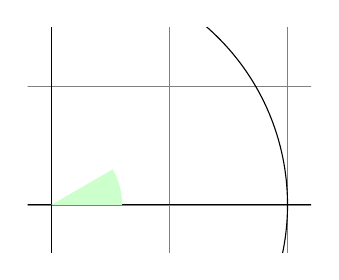
\begin{tikzpicture}[scale=3]
  \clip (-0.1,-0.2) rectangle (1.1,0.75);
  \draw[step=.5cm,gray,very thin] (-1.4,-1.4) grid (1.4,1.4);
  \draw (-1.5,0) -- (1.5,0);
  \draw (0,-1.5) -- (0,1.5);
  \draw (0,0) circle [radius=1cm];
  \fill[green!20!white] (0,0) -- (3mm,0mm)
    arc [start angle=0, end angle=30, radius=3mm] -- (0,0);
\end{tikzpicture}
\end{codeexample}

% The color |green!20!white| means 20\% green and 80\% white mixed together. Such color expression are possible since \tikzname\ uses Uwe Kern's |xcolor| package, see the documentation of that package for details on color expressions.

颜色 |green!20!white| 表示20\%的绿色和80\%的白色混合在一起。这样的颜色表达式是可能的,因为\tikzname\ 使用Uwe Kern编写的 |xcolor| 包,请参阅该包的文档以获得关于颜色表达式的详细信息。

% What would have happened, if Karl had not ``closed'' the path using |--(0,0)| at the end? In this case, the path is closed automatically, so this could have been omitted. Indeed, it would even have been better to write the following, instead:

如果卡尔没有使用 |--(0,0)|``闭合''路径在最后会发生什么?在本例中,路径会自动闭合,因此可以省略它。事实上,写以下代码甚至更好:

%
\begin{codeexample}[code only]
  \fill[green!20!white] (0,0) -- (3mm,0mm)
    arc [start angle=0, end angle=30, radius=3mm] -- cycle;
\end{codeexample}
%
%The |--cycle| causes the current path to be closed (actually the current part of the current path) by smoothly joining the first and last point. To appreciate the difference, consider the following example:

|--cycle| 通过平滑地连接第一个点和最后一个点,使当前路径闭合(事实上是当前路径的当前部分)。要了解差异,请考虑以下示例:

%
\begin{codeexample}[]
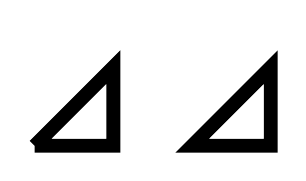
\begin{tikzpicture}[line width=5pt]
  \draw (0,0) -- (1,0) -- (1,1) -- (0,0);
  \draw (2,0) -- (3,0) -- (3,1) -- cycle;
  \useasboundingbox (0,1.5); % make bounding box higher
\end{tikzpicture}
\end{codeexample}

% You can also fill and draw a path at the same time using the |\filldraw| command. This will first draw the path, then fill it. This may not seem too useful, but you can specify different colors to be used for filling and for stroking. These are specified as optional arguments like this:

您还可以同时使用 |\filldraw| 命令来填充和绘制路径。这将首先绘制路径,然后填充它。这看起来可能不是很有用,但是你可以指定不同的颜色来填充和描边。这些被指定为可选参数,像这样:

%
\begin{codeexample}[]
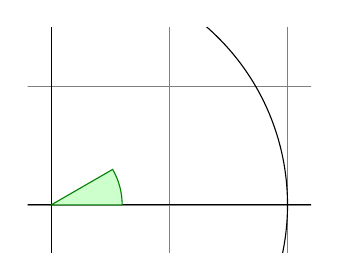
\begin{tikzpicture}[scale=3]
  \clip (-0.1,-0.2) rectangle (1.1,0.75);
  \draw[step=.5cm,gray,very thin] (-1.4,-1.4) grid (1.4,1.4);
  \draw (-1.5,0) -- (1.5,0);
  \draw (0,-1.5) -- (0,1.5);
  \draw (0,0) circle [radius=1cm];
  \filldraw[fill=green!20!white, draw=green!50!black] (0,0) -- (3mm,0mm)
    arc [start angle=0, end angle=30, radius=3mm] -- cycle;
\end{tikzpicture}
\end{codeexample}


% \subsection{Shading}
\subsection{阴影}

% Karl briefly considers the possibility of making the angle ``more fancy'' by \emph{shading} it. Instead of filling the area with a uniform color, a smooth transition between different colors is used. For this, |\shade| and |\shadedraw|, for shading and drawing at the same time, can be used:

卡尔简要地考虑了通过“阴影”使角度“更精致”的可能性。不使用统一的颜色填充区域,而是使用不同颜色之间的平滑过渡。为此,|\shade| 和 |\shadedraw| 可以同时添加阴影和进行绘图操作。

%
\begin{codeexample}[]
  \tikz \shade (0,0) rectangle (2,1)  (3,0.5) circle (.5cm);
\end{codeexample}
%
% The default shading is a smooth transition from gray to white. To specify different colors, you can use options:

默认的阴影是从灰色到白色的平滑过渡。要指定不同的颜色,您可以使用选项:

%
\begin{codeexample}[]

\begin{tikzpicture}[rounded corners,ultra thick]
  \shade[top color=yellow,bottom color=black] (0,0) rectangle +(2,1);
  \shade[left color=yellow,right color=black] (3,0) rectangle +(2,1);
  \shadedraw[inner color=yellow,outer color=black,draw=yellow] (6,0) rectangle +(2,1);
  \shade[ball color=green] (9,.5) circle (.5cm);
\end{tikzpicture}
\end{codeexample}

% For Karl, the following might be appropriate:

对于卡尔来说,以下代码可能是合适的:

%
\begin{codeexample}[]
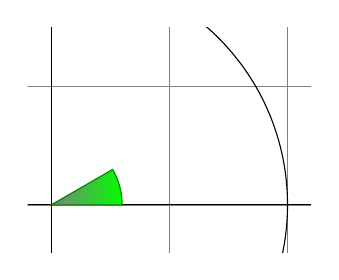
\begin{tikzpicture}[scale=3]
  \clip (-0.1,-0.2) rectangle (1.1,0.75);
  \draw[step=.5cm,gray,very thin] (-1.4,-1.4) grid (1.4,1.4);
  \draw (-1.5,0) -- (1.5,0);
  \draw (0,-1.5) -- (0,1.5);
  \draw (0,0) circle [radius=1cm];
  \shadedraw[left color=gray,right color=green, draw=green!50!black]
    (0,0) -- (3mm,0mm)
    arc [start angle=0, end angle=30, radius=3mm] -- cycle;
\end{tikzpicture}
\end{codeexample}

% However, he wisely decides that shadings usually only distract without adding anything to the picture.

然而,他明智地决定阴影通常只会分散注意力,而没有给图片添加任何东西。


%\subsection{Specifying Coordinates}
\subsection{指定坐标}

% Karl now wants to add the sine and cosine lines. He knows already that he can use the |color=| option to set the lines' colors. So, what is the best way to specify the coordinates?

卡尔现在想要加上正弦和余弦线。他已经知道可以使用 |color=| 选项来设置线条的颜色。那么,指定坐标的最好方法是什么?

% There are different ways of specifying coordinates. The easiest way is to say something like |(10pt,2cm)|. This means 10pt in $x$-direction and 2cm in $y$-directions. Alternatively, you can also leave out the units as in |(1,2)|, which means ``one times the current $x$-vector plus twice the current $y$-vector''. These vectors default to 1 cm in the $x$-direction and 1 cm in the $y$-direction, respectively.

有不同的方式来指定坐标。最简单的方法是像 |(10pt,2cm)| 这样。这意味着在$x$方向上的坐标为10pt,在$y$方向上的坐标为2cm。或者,您也可以省略单位 |(1,2)|,这意味着“当前$x$向量的1倍以及当前$y$向量的2倍”。向量默认在$x$方向上为1 cm,在$y$方向上为1 cm。

% In order to specify points in polar coordinates, use the notation |(30:1cm)|, which means 1 cm in direction 30 degree. This is obviously quite useful to ``get to the point $(\cos 30^\circ,\sin 30^\circ)$ on the circle''.

为了在极坐标中指定点,使用符号 |(30:1cm)|,意思是在30度方向上且极径为1 cm。这显然是非常有用的,以``得到圆上的点$(\cos 30^\circ,\sin 30^\circ)$''。

% You can add a single |+| sign in front of a coordinate or two of them as in |+(0cm,1cm)| or |++(2cm,0cm)|. Such coordinates are interpreted differently: The first form means ``1 cm upwards from the previous specified position'' and the second means ``2 cm to the right of the previous specified position, making this the new specified position''. For example, we can draw the sine line as follows:

您可以在坐标前添加一个或两个 |+| 符号,如 |+(0cm,1cm)| 或 |++(2cm,0cm)|。这些坐标的解释是不同的:第一种形式表示“上一指定位置上方1 cm”,第二种形式表示“上一指定位置右方2 cm,使其成为新的指定位置”。例如,我们可以画出正弦线如下:

%
\begin{codeexample}[]
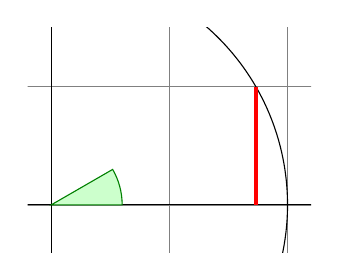
\begin{tikzpicture}[scale=3]
  \clip (-0.1,-0.2) rectangle (1.1,0.75);
  \draw[step=.5cm,gray,very thin] (-1.4,-1.4) grid (1.4,1.4);
  \draw (-1.5,0) -- (1.5,0);
  \draw (0,-1.5) -- (0,1.5);
  \draw (0,0) circle [radius=1cm];
  \filldraw[fill=green!20,draw=green!50!black] (0,0) -- (3mm,0mm)
      arc [start angle=0, end angle=30, radius=3mm] -- cycle;
  \draw[red,very thick] (30:1cm) -- +(0,-0.5);
\end{tikzpicture}
\end{codeexample}

% Karl used the fact $\sin 30^\circ = 1/2$. However, he very much doubts that his students know this, so it would be nice to have a way of specifying ``the point straight down from |(30:1cm)| that lies on the $x$-axis''. This is, indeed, possible using a special syntax: Karl can write \verb!(30:1cm |- 0,0)!. In general, the meaning of (\meta{p} \verb!|-! \meta{q}) is ``the intersection of a vertical line through $p$ and a horizontal line through $q$''.

卡尔使用了$\sin 30^\circ = 1/2$这个事实。然而,他很怀疑他的学生是否知道这一点,所以如果有一种方法来指定点从 |(30:1cm)| 径直向下绘制到在$x$轴上的点就好了。这确实是可能的,使用一种特殊的语法:Karl可以用 \verb!(30:1cm |- 0,0)!。一般来说,(\meta{p} \verb!|-! \meta{q})是“通过$p$的竖直线和通过$q$的水平线的交点”。

% Next, let us draw the cosine line. One way would be to say \verb!(30:1cm |- 0,0) -- (0,0)!. Another way is the following: we ``continue'' from where the sine ends:

接下来,我们来画余弦线。一种方法是 \verb!(30:1cm |- 0,0) -- (0,0)!。另一种方法是这样的:我们从正弦结束的地方``继续'':

%
\begin{codeexample}[]
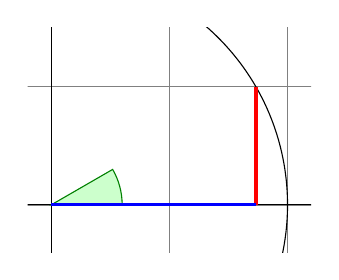
\begin{tikzpicture}[scale=3]
  \clip (-0.1,-0.2) rectangle (1.1,0.75);
  \draw[step=.5cm,gray,very thin] (-1.4,-1.4) grid (1.4,1.4);
  \draw (-1.5,0) -- (1.5,0);
  \draw (0,-1.5) -- (0,1.5);
  \draw (0,0) circle [radius=1cm];
  \filldraw[fill=green!20,draw=green!50!black] (0,0) -- (3mm,0mm)
      arc [start angle=0, end angle=30, radius=3mm] -- cycle;
  \draw[red,very thick]  (30:1cm) -- +(0,-0.5);
  \draw[blue,very thick] (30:1cm) ++(0,-0.5) -- (0,0);
\end{tikzpicture}
\end{codeexample}

% Note that there is no |--| between |(30:1cm)| and |++(0,-0.5)|. In detail, this path is interpreted as follows: ``First, the |(30:1cm)| tells me to move by pen to $(\cos 30^\circ,1/2)$. Next, there comes another coordinate specification, so I move my pen there without drawing anything. This new point is half a unit down from the last position, thus it is at $(\cos 30^\circ,0)$. Finally, I move the pen to the origin, but this time drawing something (because of the |--|).''

注意,在 |(30:1cm)| 和 |++(0,-0.5)| 之间不存在 |--|。具体来说,这个路径解释如下:``首先,|(30:1cm)| 告诉我将笔移动到$(\cos 30^\circ,1/2)$。接下来,指定了另一个坐标点,所以我移动我的笔,但不绘制任何东西。这个新点比上一个位置下降了半个单位,因此它在$(\cos 30 ^\circ,0)$。最后,我把笔移到原点,但这次画一些东西(因为用到了 |--|)。''

% To appreciate the difference between |+| and |++| consider the following example:

要理解 |+| 和 |++| 的区别,请考虑下面的例子:

%
\begin{codeexample}[]
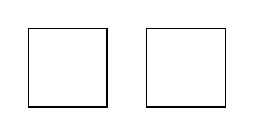
\begin{tikzpicture}
  \def\rectanglepath{-- ++(1cm,0cm)  -- ++(0cm,1cm)  -- ++(-1cm,0cm) -- cycle}
  \draw (0,0) \rectanglepath;
  \draw (1.5,0) \rectanglepath;
\end{tikzpicture}
\end{codeexample}

% By comparison, when using a single |+|, the coordinates are different:

通过比较,当使用单个 |+| 号时,坐标是不同的:

%
\begin{codeexample}[]
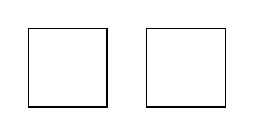
\begin{tikzpicture}
  \def\rectanglepath{-- +(1cm,0cm)  -- +(1cm,1cm)  -- +(0cm,1cm) -- cycle}
  \draw (0,0) \rectanglepath;
  \draw (1.5,0) \rectanglepath;
\end{tikzpicture}
\end{codeexample}


% Naturally, all of this could have been written more clearly and more economically like this (either with a single or a double |+|):

当然,所有这些都可以写成更清晰更经济的形式(一个或两个 |+| 号):


%
\begin{codeexample}[]
\tikz \draw (0,0) rectangle +(1,1)  (1.5,0) rectangle +(1,1);
\end{codeexample}


% \subsection{Intersecting Paths}
\subsection{相交路径}

% Karl is left with the line for $\tan \alpha$, which seems difficult to specify using transformations and polar coordinates. The first -- and easiest -- thing he can do is so simply use the coordinate |(1,{tan(30)})| since \tikzname's math engine knows how to compute things like |tan(30)|. Note the added braces since, otherwise, \tikzname's parser would think that the first closing parenthesis ends the coordinate (in general, you need to add braces around components of coordinates when these components contain parentheses).

留给卡尔的是$\tan\alpha$这一条线,这似乎很难使用变换和极坐标来指定。他能做的第一个也是最简单的事情就是使用坐标 |(1,{tan(30)})|,因为\tikzname 的数学引擎知道如何计算像 |tan(30)| 这样的东西。注意添加的大括号,否则\tikzname 的解析器会认为第一个右括号结束了坐标(通常,当坐标中包含括号时,需要坐标周围添加大括号)。

% Karl can, however, also use a more elaborate, but also more ``geometric'' way of computing the length of the orange line: He can specify intersections of paths as coordinates. The line for $\tan \alpha$ starts at $(1,0)$ and goes upward to a point that is at the intersection of a line going ``up'' and a line going from the origin through |(30:1cm)|. Such computations are made available by the |intersections| library.

但是,卡尔还可以使用更复杂但更``几何''的方式来计算橙色线的长度:他可以将路径的交点指定为坐标。 $\tan\alpha$的线从$(1,0)$开始,并向上到达一个点,该点是这条“向上”的线和一条线从原点到 |(30:1cm)| 线的交点。 通过 |intersections| 库可以得到这样的计算。 

% What Karl must do is to create two ``invisible'' paths that intersect at the position of interest. Creating paths that are not otherwise seen can be done using the |\path| command without any options like |draw| or |fill|. Then, Karl can add the |name path| option to the path for later reference. Once the paths have been constructed, Karl can use the |name intersections| to assign names to the coordinate for later reference.

卡尔必须做的是创建两条“看不见的”路径,在感兴趣的位置相交。可以使用 |\path| 命令创建其他方式看不到的路径,而不需要任何如 |draw| 或 |fill| 的选项。然后,卡尔可以将 |name path| 选项添加到该路径以供以后参考。一旦构造好了路径,卡尔就可以使用 |name intersections| 为坐标分配名称,以供以后参考。

%
\begin{codeexample}[code only]
\path [name path=upward line] (1,0) -- (1,1);
\path [name path=sloped line] (0,0) -- (30:1.5cm); % a bit longer, so that there is an intersection

% (add `\usetikzlibrary{intersections}' after loading tikz in the preamble)
\draw [name intersections={of=upward line and sloped line, by=x}]
  [very thick,orange] (1,0) -- (x);
\end{codeexample}


% \subsection{Adding Arrow Tips}
\subsection{添加箭头}

% Karl now wants to add the little arrow tips at the end of the axes. He has noticed that in many plots, even in scientific journals, these arrow tips seem to be missing, presumably because the generating programs cannot produce them. Karl thinks arrow tips belong at the end of axes. His son agrees. His students do not care about arrow tips.

卡尔现在想在轴的末端添加小箭头。 他注意到在许多情节中,甚至在科学期刊中,这些箭头似乎都消失了,大概是因为生成程序无法生成它们。卡尔认为箭头尖端位于轴的末端。 他的儿子同意。 他的学生不关心箭头。

% It turns out that adding arrow tips is pretty easy: Karl adds the option |->| to the drawing commands for the axes:

事实证明,添加箭头非常容易:卡尔在绘图命令中为坐标轴添加 |->| 选项:

%
\begin{codeexample}[preamble={\usetikzlibrary{intersections}}]
\begin{tikzpicture}[scale=3]
  \clip (-0.1,-0.2) rectangle (1.1,1.51);
  \draw[step=.5cm,gray,very thin] (-1.4,-1.4) grid (1.4,1.4);
  \draw[->] (-1.5,0) -- (1.5,0);
  \draw[->] (0,-1.5) -- (0,1.5);
  \draw (0,0) circle [radius=1cm];
  \filldraw[fill=green!20,draw=green!50!black] (0,0) -- (3mm,0mm)
        arc [start angle=0, end angle=30, radius=3mm] -- cycle;
  \draw[red,very thick]    (30:1cm) -- +(0,-0.5);
  \draw[blue,very thick]   (30:1cm) ++(0,-0.5) -- (0,0);

  \path [name path=upward line] (1,0) -- (1,1);
  \path [name path=sloped line] (0,0) -- (30:1.5cm);
  \draw [name intersections={of=upward line and sloped line, by=x}]
        [very thick,orange] (1,0) -- (x);
\end{tikzpicture}
\end{codeexample}

% If Karl had used the option |<-| instead of |->|, arrow tips would have been put at the beginning of the path. The option |<->| puts arrow tips at both ends of the path.

如果卡尔使用选项 |<-| 而不是 |->|,箭头就会被放在路径的开始处。选项 |<->| 在路径的两端都放置箭头。

% There are certain restrictions to the kind of paths to which arrow tips can be added. As a rule of thumb, you can add arrow tips only to a single open ``line''. For example, you cannot add tips to, say, a rectangle or a circle. However, you can add arrow tips to curved paths and to paths that have several segments, as in the following examples:

对于可以添加箭头的路径类型,存在某些限制。 根据经验,您只能将箭头添加到一条开放的``线''中。 例如,您不能将箭头添加到例如矩形或圆形。 但是,您可以向弯曲路径和具有多个线段的路径添加箭头,如以下示例所示:

%
\begin{codeexample}[]
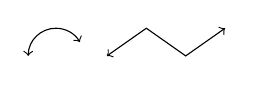
\begin{tikzpicture}
  \draw [<->] (0,0) arc [start angle=180, end angle=30, radius=10pt];
  \draw [<->] (1,0) -- (1.5cm,10pt) -- (2cm,0pt) -- (2.5cm,10pt);
\end{tikzpicture}
\end{codeexample}

% Karl has a more detailed look at the arrow that \tikzname\ puts at the end. It looks like this when he zooms it: \tikz[baseline] \draw[->,line width=1pt] (0pt,.5ex) -- ++(10pt,0pt);. The shape seems vaguely familiar and, indeed, this is exactly the end of \TeX's standard arrow used in something like $f\colon A \to B$.

卡尔详细观察发现\tikzname 把箭头放在了末端。当他放大时看起来像这样:\tikz[baseline] \draw[->,line width=1pt] (0pt,.5ex) -- ++(10pt,0pt);。形状似乎模糊不清,实际上,这恰好是\TeX 的标准箭头的末尾,用在$f\colon A \to B$之类的东西中。

% Karl likes the arrow, especially since it is not ``as thick'' as the arrows offered by many other packages. However, he expects that, sometimes, he might need to use some other kinds of arrow. To do so, Karl can say |>=|\meta{kind of end arrow tip}, where \meta{kind of end arrow tip} is a special arrow tip specification. For example, if Karl says |>=Stealth|, then he tells \tikzname\ that he would like  ``stealth-fighter-like'' arrow tips:

卡尔喜欢这个箭头,特别是因为它不是''像许多其他软件包提供的箭头''那样宽。然而,他希望,有时他可能需要使用一些其他种类的箭头。为此,卡尔可以用 |>=| \meta{末端箭头的类型},其中 \meta{末端箭头的类型} 是一个特殊的箭头规范。例如,如果卡尔用 |>=Stealth|,那么他告诉\tikzname\ 他想要“像隐形战斗机一样”的箭头:

\todosp{remaining instance of bug \#473}
%
\begin{codeexample}[preamble={\usetikzlibrary{arrows.meta}}]
\begin{tikzpicture}[>=Stealth]
  \draw [->] (0,0) arc [start angle=180, end angle=30, radius=10pt];
  \draw [<<-,very thick] (1,0) -- (1.5cm,10pt) -- (2cm,0pt) -- (2.5cm,10pt);
\end{tikzpicture}
\end{codeexample}

% Karl wonders whether such a military name for the arrow type is really necessary. He is not really mollified when his son tells him that Microsoft's PowerPoint uses the same name. He decides to have his students discuss this at some point.

卡尔想知道是否真的需要使用这种军事名称来表示箭头。 当儿子告诉他微软的PowerPoint也使用这样的名称时,他并没有真正感到高兴。 他决定让他的学生在某个时候对这个问题进行讨论。

% In addition to |Stealth| there are several other predefined kinds of arrow tips Karl can choose from, see Section~\ref{section-arrows}. Furthermore, he can define arrows types himself, if he needs new ones.

除了 |Stealth| 卡尔还可以选择其他几种预定义的箭头,请参见\ref {section-arrows}节。 此外,如果需要新的箭头类型,他可以自己定义箭头类型。


% \subsection{Scoping}
\subsection{分组}

% Karl saw already that there are numerous graphic options that affect how paths are rendered. Often, he would like to apply certain options to a whole set of graphic commands. For example, Karl might wish to draw three paths using a |thick| pen, but would like everything else to be drawn ``normally''.

卡尔已经看到,有许多图形选项会影响路径的渲染方式。 通常,他想将某些选项应用于整套图形命令。 例如,卡尔可能希望使用 |thick| 笔绘制三个路径。但希望其他所有东西都能``正常''绘制。

% If Karl wishes to set a certain graphic option for the whole picture, he can simply pass this option to the |\tikz| command or to the |{tikzpicture}| environment (Gerda would pass the options to |\tikzpicture| and Hans passes them to |\starttikzpicture|). However, if Karl wants to apply graphic options to a local group, he put these commands inside a |{scope}| environment (Gerda uses |\scope| and |\endscope|, Hans uses |\startscope| and |\stopscope|). This environment takes graphic options as an optional argument and these options apply to everything inside the scope, but not to anything outside. 

如果卡尔想为整个图片设置某个图形选项,他可以简单地将该选项传递给 |\tikz| 命令或 |{tikzpicture}| 环境(格达将把这些选项传递给 |\tikzpicture|, 汉森将它们传递给 |\starttikzpicture|)。但是,如果卡尔希望将图形选项应用到本地组,他可以将这些命令放在 |{scope}| 环境中(格达使用 |\scope| 和 |\endscope|, 汉森使用 |\startscope| 和 |\stopscope|)。该环境将图形选项作为可选参数,这些选项应用于范围内的所有内容,但不应用于范围外的任何内容。

% Here is an example:

这是一个案例:

%
\begin{codeexample}[]
\begin{tikzpicture}[ultra thick]
  \draw (0,0) -- (0,1);
  \begin{scope}[thin]
    \draw (1,0) -- (1,1);
    \draw (2,0) -- (2,1);
  \end{scope}
  \draw (3,0) -- (3,1);
\end{tikzpicture}
\end{codeexample}

% Scoping has another interesting effect: Any changes to the clipping area are local to the scope. Thus, if you say |\clip| somewhere inside a scope, the effect of the |\clip| command ends at the end of the scope. This is useful since there is no other way of ``enlarging'' the clipping area.

分组还有另一个有趣的作用:裁剪区域的任何更改都是该分组的局部更改。因此,如果您用 |\clip| 在某个分组内的某个地方,|\clip| 命令的效果将在分组的末尾结束。这是有用的,因为没有其他方式``扩大''剪切区域。

% Karl has also already seen that giving options to commands like |\draw| apply only to that command. It turns out that the situation is slightly more complex. First, options to a command like |\draw| are not really options to the command, but they are ``path options'' and can be given anywhere on the path. So, instead of |\draw[thin] (0,0) -- (1,0);| one can also write |\draw (0,0) [thin] -- (1,0);| or |\draw (0,0) -- (1,0) [thin];|; all of these have the same effect. This might seem strange since in the last case, it would appear that the |thin| should take effect only ``after'' the line from $(0,0)$ to $(1,0)$ has been drawn. However, most graphic options only apply to the whole path. Indeed, if you say both |thin| and |thick| on the same path, the last option given will ``win''.

卡尔也已经看到给像 |\draw| 这样的命令提供选项只适用于该命令。事实证明,情况要稍微复杂一些。首先,像 |\draw| 这样的命令的选项实际上并不是该命令的选项,但它们是“路径选项”,可以在路径的任何位置提供。因此,除了用 |\draw[thin] (0,0) -- (1,0);| 还可以用 |\draw (0,0) [thin] -- (1,0);| 或 |\draw (0,0) -- (1,0) [thin];|;所有这些都会产生同样的效果。这看起来可能有些奇怪,因为在上一种情况下,看起来 |thin| 应该只在从$(0,0)$到$(1,0)$这一行的``之后''才生效。但是,大多数图形选项只适用于整个路径。事实上,如果你将 |thin| 和 |thick| 用在同一条路径上,给出的最后一个选项将会``赢得胜利''。

% When reading the above, Karl notices that only ``most'' graphic options apply to the whole path. Indeed, all transformation options do \emph{not} apply to the whole path, but only to ``everything following them on the path''. We will have a more detailed look at this in a moment. Nevertheless, all options given during a path construction apply only to this path.

阅读以上内容时,卡尔注意到只有``大多数''图形选项适用于整个路径。 确实,所有变换选项都\emph{不会}适用于整个路径,而仅适用于``路径上遵循它们的所有内容''。 稍后我们将对此进行更详细的介绍。 但是,在路径构建过程中给出的所有选项仅适用于该路径。

% \subsection{Transformations}
\subsection{坐标变换}

% When you specify a  coordinate like |(1cm,1cm)|, where is that coordinate placed on the page? To determine the position, \tikzname, \TeX, and \textsc{pdf} or PostScript all apply certain transformations to the given coordinate in order to determine the final position on the page.

当您指定 |(1cm,1cm)| 之类的坐标时,该坐标在页面上的什么位置? 为了确定位置,\tikzname\ , \TeX 和\textsc{pdf}或PostScript都会使用一种确定的坐标变换,以确定其在页面上的最终位置。

% \tikzname\ provides numerous options that allow you to transform coordinates in \tikzname's private coordinate system. For example, the |xshift| option allows you to shift all subsequent points by a certain amount:

\tikzname\ 提供了许多选项,允许您在\tikzname 的私有坐标系统中变换坐标。例如,|xshift| 选项允许您将所有后续点移动一定距离:

\begin{codeexample}[]
\tikz \draw (0,0) -- (0,0.5) [xshift=2pt] (0,0) -- (0,0.5);
\end{codeexample}

% It is important to note that you can change transformation ``in the middle of a path'', a feature that is not supported by \pdf\ or PostScript. The reason is that \tikzname\ keeps track of its own transformation matrix. 

需要注意的是,您可以在``路径的中间''坐标变换,\pdf\ 或PostScript不支持这一特性。原因是\tikzname\ 会持续跟踪自己的坐标变换矩阵。

% Here is a more complicated example:

这是一个更复杂的示例:

%
\begin{codeexample}[]

\begin{tikzpicture}[even odd rule,rounded corners=2pt,x=10pt,y=10pt]
  \filldraw[fill=yellow!80!black] (0,0)   rectangle (1,1)
        [xshift=5pt,yshift=5pt]   (0,0)   rectangle (1,1)
                    [rotate=30]   (-1,-1) rectangle (2,2);
\end{tikzpicture}
\end{codeexample}

% The most useful transformations are |xshift| and |yshift| for shifting, |shift| for shifting to a given point as in |shift={(1,0)}| or |shift={+(0,0)}| (the braces are necessary so that \TeX\ does not mistake the comma for separating options), |rotate| for rotating by a certain angle (there is also a |rotate around| for rotating around a given point), |scale| for scaling by a certain factor, |xscale| and |yscale| for scaling only in the $x$- or $y$-direction (|xscale=-1| is a flip), and |xslant| and |yslant| for slanting. If these transformation and those that I have not mentioned are not sufficient, the |cm| option allows you to apply an arbitrary transformation matrix. Karl's students, by the way, do not know what a transformation matrix is.

最有用的坐标变换是用于平移的 |xshift| 和 |yshift| 变换,|shift| 变换将指定图形平移\verb|shift={(1,0)}|或 \verb|shift={+(0,0)}|中给定的距离(大括号是必需的,以便\TeX\ 不会将逗号分隔为选项),|rotate| 变换将指定图形旋转指定的角度(还有一个 |rotate around| 用于绕给定点旋转),|xscale| 和 |yscale| 用于将指定图形在$x$或$y$方向上缩放指定的倍数,|xslant| 和 |yslant| 用于图形的倾斜。如果这些变换以及我没有提到的变换都不足够,那么 |cm| 选项允许您应用任意变换矩阵。 顺便说一下,卡尔的学生不知道什么是变换矩阵。


% \subsection{Repeating Things: For-Loops}
\subsection{重复工作:For循环}

% Karl's next aim is to add little ticks on the axes at positions $-1$, $-1/2$, $1/2$, and $1$. For this, it would be nice to use some kind of ``loop'', especially since he wishes to do the same thing at each of these positions. There are different packages for doing this. \LaTeX\ has its own internal command for this, |pstricks| comes along with the powerful |\multido| command. All of these can be used together with \tikzname, so if you are familiar with them, feel free to use them. \tikzname\ introduces yet another command, called |\foreach|, which I introduced since I could never remember the syntax of the other packages. |\foreach| is defined in the package |pgffor| and can be used independently of \tikzname, but \tikzname\ includes it automatically.

卡尔的下一个目标是在$-1$,$-1/2$,$1/2$和$1$的位置的坐标轴上添加小刻度。为此,最好使用某种‘循环’,特别是因为他希望在这些位置上做同样的事情。可以使用不同的包来完成这项工作。\LaTeX\ 对此有自己的内部命令,|pstricks| 带有强大的 |\multido| 命令。所有这些都可以与\tikzname 一起使用,所以如果您熟悉它们,可以随意使用它们。\tikzname\ 引入了另一个命令 |\foreach|,我引入这个命令是因为我永远记不住其他宏包的语法。|\foreach| 命令定义在宏包 |pgffor| 中,可以独立于\tikzname 使用,但\tikzname\ 会自动包含它。

% In its basic form, the |\foreach| command is easy to use:

|\foreach| 命令的基本形式很容易使用:

%
\begin{codeexample}[]
\foreach \x in {1,2,3} {$x =\x$, }
\end{codeexample}

% The general syntax is |\foreach| \meta{variable}| in {|\meta{list of values}|} |\meta{commands}. Inside the \meta{commands}, the \meta{variable} will be assigned to the different values. If the \meta{commands} do not start with a brace, everything up to the next semicolon is used as \meta{commands}.

一般语法是 |\foreach| \meta{变量}| in {|\meta{值清单}|} |\meta{命令}。在\meta{命令} 内部,\meta{变量} 将分配给不同的值。如果 \meta{命令} 不是以大括号开头,则直到下一个分号的所有内容都将用作 \meta{命令}。

% For Karl and the ticks on the axes, he could use the following code:

对于卡尔,他可以使用以下代码绘制坐标轴上的刻度:

%
\begin{codeexample}[]
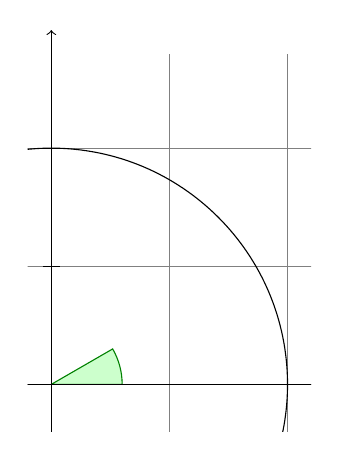
\begin{tikzpicture}[scale=3]
  \clip (-0.1,-0.2) rectangle (1.1,1.51);
  \draw[step=.5cm,gray,very thin] (-1.4,-1.4) grid (1.4,1.4);
  \filldraw[fill=green!20,draw=green!50!black] (0,0) -- (3mm,0mm)
      arc [start angle=0, end angle=30, radius=3mm] -- cycle;
  \draw[->] (-1.5,0) -- (1.5,0);
  \draw[->] (0,-1.5) -- (0,1.5);
  \draw (0,0) circle [radius=1cm];

  \foreach \x in {-1cm,-0.5cm,1cm}
    \draw (\x,-1pt) -- (\x,1pt);
  \foreach \y in {-1cm,-0.5cm,0.5cm,1cm}
    \draw (-1pt,\y) -- (1pt,\y);
\end{tikzpicture}
\end{codeexample}

% As a matter of fact, there are many different ways of creating the ticks. For example, Karl could have put the |\draw ...;| inside curly braces. He could also have used, say,

实际上,创建刻度线有很多不同的方法。 例如,卡尔可以将 |\draw ...;| 放在大括号内。 他还可以用,比如说,这样

%
\begin{codeexample}[code only]
\foreach \x in {-1,-0.5,1}
  \draw[xshift=\x cm] (0pt,-1pt) -- (0pt,1pt);
\end{codeexample}

% Karl is curious what would happen in a more complicated situation where there are, say, 20 ticks. It seems bothersome to explicitly mention all these numbers in the set for |\foreach|. Indeed, it is possible to use |...| inside the |\foreach| statement to iterate over a large number of values (which must, however, be dimensionless real numbers) as in the following example:

卡尔很好奇在更复杂的情况下会发生什么,比如说,20个刻度。为每个 |\foreach| 明确地提到集合中的所有数字似乎很麻烦。事实上,可以在 |\foreach| 声明中使用 |...| 产生大量迭代值(但是,它必须是无量纲的实数),如以下示例所示:

%
\begin{codeexample}[]
\tikz \foreach \x in {1,...,10}
        \draw (\x,0) circle (0.4cm);
\end{codeexample}

% If you provide \emph{two} numbers before the |...|, the |\foreach| statement will use their difference for the stepping:

如果在 |...| 之前提供\emph{2个}数字,则 |\foreach| 语句根据它们的差值进行步进:

%
\begin{codeexample}[]
\tikz \foreach \x in {-1,-0.5,...,1}
       \draw (\x cm,-1pt) -- (\x cm,1pt);
\end{codeexample}

% We can also nest loops to create interesting effects:

我们还可以使用嵌套循环以产生有趣的效果:

%
\begin{codeexample}[]
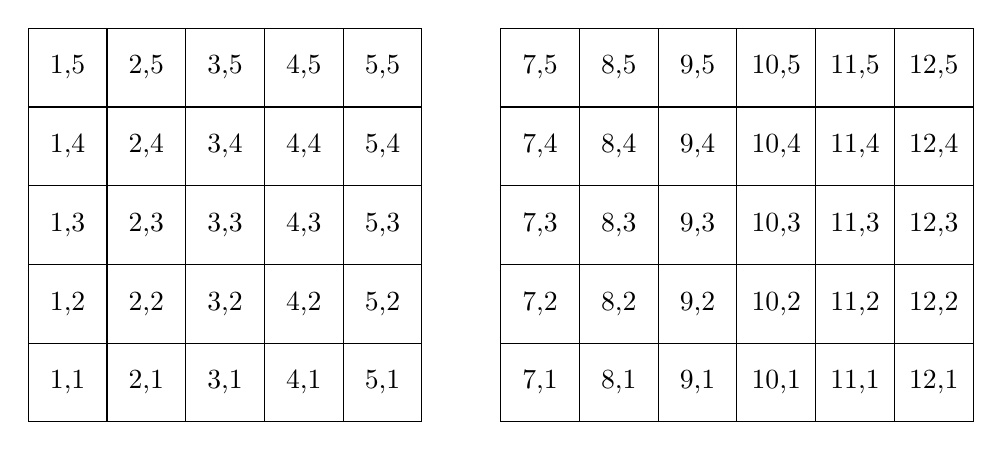
\begin{tikzpicture}
  \foreach \x in {1,2,...,5,7,8,...,12}
    \foreach \y in {1,...,5}
    {
      \draw (\x,\y) +(-.5,-.5) rectangle ++(.5,.5);
      \draw (\x,\y) node{\x,\y};
    }
\end{tikzpicture}
\end{codeexample}

% The |\foreach| statement can do even trickier stuff, but the above gives the idea.

|\foreach| 语句甚至可以做更棘手的事情,但是上面已经给出了这个想法。


% \subsection{Adding Text}
\subsection{添加文本}

% Karl is, by now, quite satisfied with the picture. However, the most important parts, namely the labels, are still missing!

到目前为止,卡尔对图片非常满意。 但是,最重要的部分,即文字标签,仍然缺失!

% \tikzname\ offers an easy-to-use and powerful system for adding text and, more generally, complex shapes to a picture at specific positions. The basic idea is the following: When \tikzname\ is constructing a path and encounters the keyword |node| in the middle of a path, it reads a \emph{node specification}. The keyword |node| is typically followed by some options and then some text between curly braces. This text is put inside a normal \TeX\ box (if the node specification directly follows a coordinate, which is usually the case, \tikzname\ is able to perform some magic so that it is even possible to use verbatim text inside the boxes) and then placed at the current position, that is, at the last specified position (possibly shifted a bit, according to the given options). However, all nodes are drawn only after the path has been completely drawn/filled/shaded/clipped/whatever.

\tikzname\ 提供了一个易于使用且功能强大的系统,用于在特定位置向图片添加文本和复杂形状。其基本思想如下:当\tikzname\ 构造路径并在路径中间遇到关键字 |node| 时,它读取\emph{节点详述}。关键字 |node| 后面通常跟着一些选项以及放在花括号之间的文本。这段文字放在普通的\TeX\ 盒子中(如果节点规范直接遵循坐标,并且通常就是这种情况,\tikzname\ 可以执行一些魔法般的操作,从而甚至可以在框中使用逐字记录文本),然后放在当前位置,即最后指定的位置(根据给定的选项,可能会移动一点)。但是,仅在完全绘制/填充/阴影/剪切或任何路径之后才绘制所有节点。

%
\begin{codeexample}[]
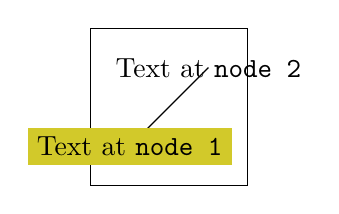
\begin{tikzpicture}
  \draw (0,0) rectangle (2,2);
  \draw (0.5,0.5) node [fill=yellow!80!black]
                       {Text at \verb!node 1!}
     -- (1.5,1.5) node {Text at \verb!node 2!};
\end{tikzpicture}
\end{codeexample}

% Obviously, Karl would not only like to place nodes \emph{on} the last specified position, but also to the left or the right of these positions. For this, every node object that you put in your picture is equipped with several \emph{anchors}. For example, the |north| anchor is in the middle at the upper end of the shape, the |south| anchor is at the bottom and the |north east| anchor is in the upper right corner. When you give the option |anchor=north|, the text will be placed such that this northern anchor will lie on the current position and the text is, thus, below the current position. Karl uses this to draw the ticks as follows:

显然,卡尔不仅希望将节点\emph{放置}在最后指定的位置,而是希望将其放置在这些位置的左侧或右侧。为此,你在图片中放置的每个节点对象都配备了多个\emph{锚点}。例如,|north| 锚点位于形状上端的中间,|south| 的锚点位于形状的底部,|north east| 的锚点位于形状的右上角。当提供选项 |anchor=north| 时,将放置文本,使得该北锚位于当前位置,因此该文本位于当前位置的下方。卡尔使用此方法绘制刻度线,如下所示:

%
\begin{codeexample}[]
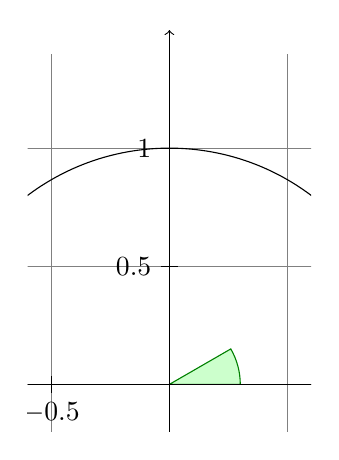
\begin{tikzpicture}[scale=3]
  \clip (-0.6,-0.2) rectangle (0.6,1.51);
  \draw[step=.5cm,help lines] (-1.4,-1.4) grid (1.4,1.4);
  \filldraw[fill=green!20,draw=green!50!black] (0,0) -- (3mm,0mm)
    arc [start angle=0, end angle=30, radius=3mm] -- cycle;
  \draw[->] (-1.5,0) -- (1.5,0);   \draw[->] (0,-1.5) -- (0,1.5);
  \draw (0,0) circle [radius=1cm];

  \foreach \x in {-1,-0.5,1}
    \draw (\x cm,1pt) -- (\x cm,-1pt) node[anchor=north] {$\x$};
  \foreach \y in {-1,-0.5,0.5,1}
    \draw (1pt,\y cm) -- (-1pt,\y cm) node[anchor=east] {$\y$};
\end{tikzpicture}
\end{codeexample}

% This is quite nice, already. Using these anchors, Karl can now add most of the other text elements. However, Karl thinks that, though ``correct'', it is quite counter-intuitive that in order to place something \emph{below} a given point, he has to use the \emph{north} anchor. For this reason, there is an option called |below|, which does the same as |anchor=north|. Similarly, |above right| does the same as |anchor=south west|. In addition, |below| takes an optional dimension argument. If given, the shape will additionally be shifted downwards by the given amount. So, |below=1pt| can be used to put a text label below some point and, additionally shift it  1pt downwards.

这已经很不错了。使用这些锚点,卡尔现在可以添加大多数的其他文本元素。然而,卡尔认为,虽然“正确”,但这是违反直觉的,为了把某些东西放在一个给定的点下面,他必须使用\emph{north}锚点。因此,有一个 |below| 的选项,它的作用与 |anchor=north| 相同。类似地,|above right| 与 |anchor=south wes| 的作用相同。另外,|below| 选项有一个可选的尺寸参数。如果给定,该形状将额外向下移动给定的数量。因此,|bellow=1pt| 可以用来把一个文本标签放在某个点下面,另外,将它向下移动1pt。

% Karl is not quite satisfied with the ticks. He would like to have $1/2$ or $\frac{1}{2}$ shown instead of $0.5$, partly to show off the nice capabilities of \TeX\ and \tikzname, partly because for positions like $1/3$ or $\pi$ it is certainly very much preferable to have the ``mathematical'' tick there instead of just the ``numeric'' tick. His students, on the other hand, prefer $0.5$ over $1/2$ since they are not too fond of fractions in general.

卡尔对刻度不太满意。他希望显示$1/2$或$\frac{1}{2}$而不是$0.5$,部分原因是为了展示\TeX\ 和\tikzname 的出色功能,部分原因是对于$1/3$或$\pi$这样的刻度,在上面放置``数学''的刻度而不是仅``数字的''刻度当然是更加可取的。 另一方面,他的学生更喜欢$0.5$而不是$1/2$,因为他们一般不太喜欢分数。

% Karl now faces a problem: For the |\foreach| statement, the position |\x| should still be given as |0.5| since \tikzname\ will not know where |\frac{1}{2}| is supposed to be. On the other hand, the typeset text should really be  |\frac{1}{2}|. To solve this problem, |\foreach| offers a special syntax: Instead of having one variable |\x|, Karl can specify two (or even more) variables separated by a slash as in |\x / \xtext|. Then, the elements in the set over which |\foreach| iterates must also be of the form \meta{first}|/|\meta{second}. In each iteration, |\x| will be set to \meta{first} and |\xtext| will be set to \meta{second}. If no \meta{second} is given, the \meta{first} will be used again. So, here is the new code for the ticks:

卡尔现在面临一个问题:对于 |\foreach| 声明,位置 |\x| 仍应为 |0.5|,因为\tikzname\ 不知道应该是 |\frac{1}{2}|。但另一方面,排版文本实际上应该是 |\frac{1}{2}|。要解决此问题,|\foreach| 提供了一种特殊的语法:与其使用一个变量 |\x|,卡尔可以指定两个(或更多)用斜杠分隔的变量 |\x / \xtext|。然后,集合中的元素使用 |\foreach| 迭代也必须采用 \meta{first}|/|\meta{second} 的形式。在每次迭代中,|\x| 将设置为 \meta{first},|\xtext| 将设置为 \meta{second}。如果没有给出 \meta{second},将再次使用 \meta{first}。因此,这是刻度的新代码:

%
\begin{codeexample}[]
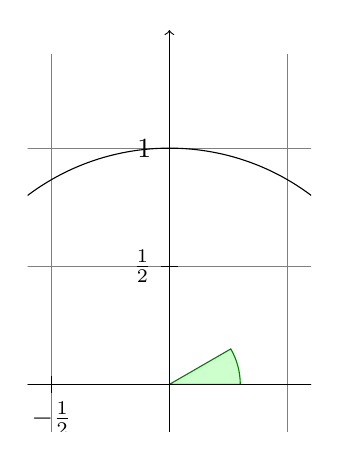
\begin{tikzpicture}[scale=3]
  \clip (-0.6,-0.2) rectangle (0.6,1.51);
  \draw[step=.5cm,help lines] (-1.4,-1.4) grid (1.4,1.4);
  \filldraw[fill=green!20,draw=green!50!black] (0,0) -- (3mm,0mm)
      arc [start angle=0, end angle=30, radius=3mm] -- cycle;
  \draw[->] (-1.5,0) -- (1.5,0); \draw[->] (0,-1.5) -- (0,1.5);
  \draw (0,0) circle [radius=1cm];

  \foreach \x/\xtext in {-1, -0.5/-\frac{1}{2}, 1}
    \draw (\x cm,1pt) -- (\x cm,-1pt) node[anchor=north] {$\xtext$};
  \foreach \y/\ytext in {-1, -0.5/-\frac{1}{2}, 0.5/\frac{1}{2}, 1}
    \draw (1pt,\y cm) -- (-1pt,\y cm) node[anchor=east] {$\ytext$};
\end{tikzpicture}
\end{codeexample}

% Karl is quite pleased with the result, but his son points out that this is still not perfectly satisfactory: The grid and the circle interfere with the numbers and decrease their legibility. Karl is not very concerned by this (his students do not even notice), but his son insists that there is an easy solution: Karl can add the |[fill=white]| option to fill out the background of the text shape with a white color.

卡尔对结果感到非常满意,但是他的儿子指出这仍然不能令人满意:网格和圆会干扰数字并降低其可读性。  卡尔对此并不十分担心(他的学生甚至没有注意到),但是他的儿子坚持认为有一个简单的解决方案:卡尔可以添加 \verb|[fill=white]| 选项,用白色填充文本形状的背景。

% The next thing Karl wants to do is to add the labels like $\sin \alpha$. For this, he would like to place a label ``in the middle of the line''. To do so, instead of specifying the label |node {$\sin\alpha$}|  directly after one of the endpoints of the line (which would place the label at that endpoint), Karl can give the label directly after the |--|, before the coordinate. By default, this places the label in the middle of the line, but the |pos=| options can be used to modify this. Also, options like |near start| and |near end| can be used to modify this position:

卡尔接下来要做的就是添加$\sin\alpha$之类的标签。为此,他想在线的中间放置一个标签。这样做,而不是指定标签 |node {$\sin\alpha$}| 直接在直线的一个端点之后(即将标签放置在端点处),卡尔可以在 |--| 之后,在坐标之前直接给出标签。缺省情况下,这会将标签放在行的中间,但是 |pos=| 选项可以用来修改它。另外,|near start| 和 |near end| 可以用来修改这个位置:
%
\begin{codeexample}[preamble={\usetikzlibrary{intersections}}]
\begin{tikzpicture}[scale=3]
  \clip (-2,-0.2) rectangle (2,0.8);
  \draw[step=.5cm,gray,very thin] (-1.4,-1.4) grid (1.4,1.4);
  \filldraw[fill=green!20,draw=green!50!black] (0,0) -- (3mm,0mm)
    arc [start angle=0, end angle=30, radius=3mm] -- cycle;
  \draw[->] (-1.5,0) -- (1.5,0) coordinate (x axis);
  \draw[->] (0,-1.5) -- (0,1.5) coordinate (y axis);
  \draw (0,0) circle [radius=1cm];

  \draw[very thick,red]
    (30:1cm) -- node[left=1pt,fill=white] {$\sin \alpha$} (30:1cm |- x axis);
  \draw[very thick,blue]
    (30:1cm |- x axis) -- node[below=2pt,fill=white] {$\cos \alpha$} (0,0);
  \path [name path=upward line] (1,0) -- (1,1);
  \path [name path=sloped line] (0,0) -- (30:1.5cm);
  \draw [name intersections={of=upward line and sloped line, by=t}]
    [very thick,orange] (1,0) -- node [right=1pt,fill=white]
    {$\displaystyle \tan \alpha \color{black}=
      \frac{{\color{red}\sin \alpha}}{\color{blue}\cos \alpha}$} (t);

  \draw (0,0) -- (t);

  \foreach \x/\xtext in {-1, -0.5/-\frac{1}{2}, 1}
    \draw (\x cm,1pt) -- (\x cm,-1pt) node[anchor=north,fill=white] {$\xtext$};
  \foreach \y/\ytext in {-1, -0.5/-\frac{1}{2}, 0.5/\frac{1}{2}, 1}
    \draw (1pt,\y cm) -- (-1pt,\y cm) node[anchor=east,fill=white] {$\ytext$};
\end{tikzpicture}
\end{codeexample}

% You can also position labels on curves and, by adding the |sloped| option, have them rotated such that they match the line's slope. Here is an example:

您也可以在曲线上放置标签,并通过添加 |sloped| 选项,使其旋转以使其与直线的斜率匹配。 这是一个例子:

%

\begin{codeexample}[]
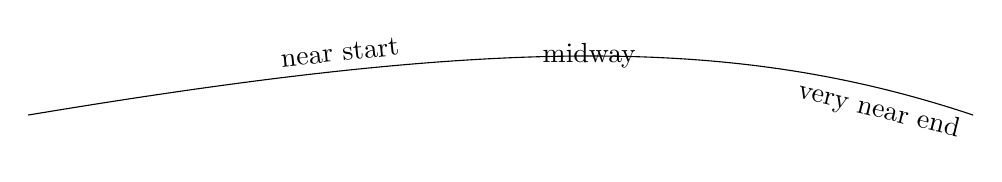
\begin{tikzpicture}
  \draw (0,0) .. controls (6,1) and (9,1) ..
    node[near start,sloped,above] {near start}
    node {midway}
    node[very near end,sloped,below] {very near end} (12,0);
\end{tikzpicture}
\end{codeexample}

% It remains to draw the explanatory text at the right of the picture. The main difficulty here lies in limiting the width of the text ``label'', which is quite long, so that line breaking is used. Fortunately, Karl can use the option |text width=6cm| to get the desired effect. So, here is the full code:

现在仍然需要在图片右侧绘制说明文字。 这里的主要困难在于限制文本``标签''的宽度,该宽度相当长,因为使用了换行符。幸运的是,卡尔可以使用选项 |text width=6cm|,以获得理想的效果。 因此,这是完整的代码:
%
\begin{codeexample}[code only]
\begin{tikzpicture}
  [scale=3,line cap=round,
  % Styles
  axes/.style=,
  important line/.style={very thick},
  information text/.style={rounded corners,fill=red!10,inner sep=1ex}]

  % Colors
  \colorlet{anglecolor}{green!50!black}
  \colorlet{sincolor}{red}
  \colorlet{tancolor}{orange!80!black}
  \colorlet{coscolor}{blue}

  % The graphic
  \draw[help lines,step=0.5cm] (-1.4,-1.4) grid (1.4,1.4);

  \draw (0,0) circle [radius=1cm];

  \begin{scope}[axes]
    \draw[->] (-1.5,0) -- (1.5,0) node[right] {$x$} coordinate(x axis);
    \draw[->] (0,-1.5) -- (0,1.5) node[above] {$y$} coordinate(y axis);

    \foreach \x/\xtext in {-1, -.5/-\frac{1}{2}, 1}
      \draw[xshift=\x cm] (0pt,1pt) -- (0pt,-1pt) node[below,fill=white] {$\xtext$};

    \foreach \y/\ytext in {-1, -.5/-\frac{1}{2}, .5/\frac{1}{2}, 1}
      \draw[yshift=\y cm] (1pt,0pt) -- (-1pt,0pt) node[left,fill=white] {$\ytext$};
  \end{scope}

  \filldraw[fill=green!20,draw=anglecolor] (0,0) -- (3mm,0pt)
    arc [start angle=0, end angle=30, radius=3mm];
  \draw (15:2mm) node[anglecolor] {$\alpha$};

  \draw[important line,sincolor]
    (30:1cm) -- node[left=1pt,fill=white] {$\sin \alpha$} (30:1cm |- x axis);

  \draw[important line,coscolor]
    (30:1cm |- x axis) -- node[below=2pt,fill=white] {$\cos \alpha$} (0,0);

  \path [name path=upward line] (1,0) -- (1,1);
  \path [name path=sloped line] (0,0) -- (30:1.5cm);
  \draw [name intersections={of=upward line and sloped line, by=t}]
    [very thick,orange] (1,0) -- node [right=1pt,fill=white]
    {$\displaystyle \tan \alpha \color{black}=
      \frac{{\color{red}\sin \alpha}}{\color{blue}\cos \alpha}$} (t);

  \draw (0,0) -- (t);

  \draw[xshift=1.85cm]
    node[right,text width=6cm,information text]
    {
      The {\color{anglecolor} angle $\alpha$} is $30^\circ$ in the
      example ($\pi/6$ in radians). The {\color{sincolor}sine of
        $\alpha$}, which is the height of the red line, is
      \[
      {\color{sincolor} \sin \alpha} = 1/2.
      \]
      By the Theorem of Pythagoras ...
    };
\end{tikzpicture}
\end{codeexample}


%\subsection{Pics: The Angle Revisited}
\subsection{Pics:再访Angle}

% Karl expects that the code of certain parts of the picture he created might be so useful that he might wish to reuse them in the future. A natural thing to do is to create \TeX\ macros that store the code he wishes to reuse. However, \tikzname\ offers another way that is integrated directly into its parser: pics!

卡尔希望他创建的图片某些部分的代码可能会非常有用,以至于他将来希望重用它们。 自然的做法是创建\TeX\ 宏来存储他希望重用的代码。 但是,\tikzname\ 提供了另一种直接集成到其解析器中的方式:图片!

% A ``pic'' is ``not quite a full picture'', hence the short name. The idea is that a pic is simply some code that you can add to a picture at different places using the |pic| command whose syntax is almost identical to the |node| command. The main difference is that instead of specifying some text in curly braces that should be shown, you specify the name of a predefined picture that should be shown.

``pic''是一种``不是很完整的图片'',因此我们使用简称。 这个想法是,图片只是一些代码,您可以使用 |pic| 命令添加到图片的不同位置, 它的语法几乎与 |node| 命令相同。 主要区别在于,您可以指定应该显示的预定义图片的名称,而不是在花括号中指定一些文本。

% Defining new pics is easy enough, see Section~\ref{section-pics}, but right now we just want to use one such predefined pic: the |angle| pic. As the name suggests, it is a small drawing of an angle consisting of a little wedge and an arc together with some text (Karl needs to load the |angles| library and the |quotes| for the following examples). What makes this pic useful is the fact that the size of the wedge will be computed automatically.

定义新的pics很容易,请参见\ref{section-pics}节,但是现在我们只想使用一个这样的预定义的pic:|angle| pic。顾名思义,这是一个由一张由一个楔形和一段弧以及一些文本组成的小图形(在以下示例中,卡尔需要加载 |angles| 和 |quotes| 库)。pic很有用的原因是,楔形的大小会被自动计算。

% The |angle| pic draws an angle between the two lines $BA$ and $BC$, where $A$, $B$, and $C$ are three coordinates. In our case, $B$ is the origin, $A$ is somewhere on the $x$-axis and $C$ is somewhere on a line at $30^\circ$.

|angle| pic在$BA$和$BC$两条线之间绘制一个角度,其中$A$、$B$和$C$是三个坐标。在我们的例子中,$B$是原点,$A$在$x$轴的某处,$C$在$30^\circ$这条线上的某处。
%
\begin{codeexample}[preamble={\usetikzlibrary{angles,quotes}}]
\begin{tikzpicture}[scale=3]
  \coordinate (A) at (1,0);
  \coordinate (B) at (0,0);
  \coordinate (C) at (30:1cm);

  \draw (A) -- (B) -- (C)
        pic [draw=green!50!black, fill=green!20, angle radius=9mm,
             "$\alpha$"] {angle = A--B--C};
\end{tikzpicture}
\end{codeexample}

% Let us see, what is happening here. First we have specified three \emph{coordinates} using the |\coordinate| command. It allows us to name a specific coordinate in the picture. Then comes something that starts as a normal |\draw|, but then comes the |pic| command. This command gets lots of options and, in curly braces, comes the most important point: We specify that we want to add an |angle| pic and this angle should be between the points we named |A|, |B|, and |C| (we could use other names). Note that the text that we want to be shown in the pic is specified in quotes inside the options of the |pic|, not inside the curly braces.

让我们来看看,这里发生了什么。首先,我们使用 |\coordinate| 命令指定了三个\emph{坐标点}。它允许我们在图片中对一个特定的坐标命名。然后是一个普通的 |\draw| 命令,然后是 |pic| 命令。这个命令有很多选项,在花括号中是最重要的一点:我们指定要添加一个 |angle| pic,这个角应该位于我们命名的 |A|、|B| 和 |C| 之间(我们也可以使用其他名称)。注意,我们希望在pic中显示的文本是在 |pic| 选项中的引号中指定的,而不是在花括号中。

% To learn more about pics, please see Section~\ref{section-pics}.

要了解有关pics的更多信息,请参见\ref{section-pics}节。

\clearpage
% Copyright 2006 by Till Tantau
%
% This file may be distributed and/or modified
%
% 1. under the LaTeX Project Public License and/or
% 2. under the GNU Free Documentation License.
%
% See the file doc/generic/pgf/licenses/LICENSE for more details.


% \section{Tutorial: A Petri-Net for Hagen}
\section{教程:哈根的Petri网}

% In this second tutorial we explore the node mechanism of \tikzname\ and \pgfname.

在第二篇教程中,我们探讨\tikzname\ 和\pgfname 节点的原理。

% Hagen must give a talk tomorrow about his favorite formalism for distributed systems: Petri nets! Hagen used to give his talks using a blackboard and everyone seemed to be perfectly content with this. Unfortunately, his audience has been spoiled recently with fancy projector-based presentations and there seems to be a certain amount of peer pressure that his Petri nets should also be drawn using a graphic program. One of the professors at his institute recommends \tikzname\ for this and Hagen decides to give it a try.

哈根(Hagen)明天需要就他最喜欢的分布式系统形式:Petri网发表演讲。 哈根以前常常用黑板发表演讲,每个人似乎对此都很满意。 不幸的是,他的听众最近迷恋上了基于投影仪的奇特演示,似乎还有一定的同行压力,要求他的Petri网的图形也应使用图形程序绘制。 为此,他所在学院的一位教授推荐了\tikzname\ ,哈根决定尝试一下。


% \subsection{Problem Statement}
\subsection{问题陈述}

% For his talk, Hagen wishes to create a graphic that demonstrates how a net with place capacities can be simulated by a net without capacities. The graphic should look like this, ideally:

对于他的演讲,哈根希望创建一个图形来演示如何通过无库所容量的网络模拟有库所容量的网络。 图形在理想情况下应该看起来像这样:{\color{red}\ref{error}}

%
\begin{quote}
\begin{tikzpicture}
  [node distance=1.3cm,>={Stealth[round]},bend angle=45,auto,
   place/.style={circle,thick,draw=blue!75,fill=blue!20,minimum size=6mm},
   red place/.style={place,draw=red!75,fill=red!20},
   transition/.style={rectangle,thick,draw=black!75,fill=black!20,minimum size=4mm},
   every label/.style={red},on grid]

  \begin{scope}
    % First net
    \node [place,tokens=1] (w1)                                    {};
    \node [place] (c1) [below=of w1]                      {};
    \node [place] (s)  [below=of c1,label=above:$s\le 3$] {};
    \node [place] (c2) [below=of s]                       {};
    \node [place,tokens=1] (w2) [below=of c2]                      {};

    \node [transition] (e1) [left=of c1] {}
      edge [pre,bend left]                  (w1)
      edge [post,bend right]                (s)
      edge [post]                           (c1);

    \node [transition] (e2) [left=of c2] {}
      edge [pre,bend right]                 (w2)
      edge [post,bend left]                 (s)
      edge [post]                           (c2);

    \node [transition] (l1) [right=of c1] {}
      edge [pre]                            (c1)
      edge [pre,bend left]                  (s)
      edge [post,bend right] node[swap] {2} (w1);

    \node [transition] (l2) [right=of c2] {}
      edge [pre]                            (c2)
      edge [pre,bend right]                 (s)
      edge [post,bend left]  node {2}       (w2);
  \end{scope}

  \begin{scope}[xshift=6cm]
    % Second net
    \node [place,tokens=1]
                      (w1')                                                {};
    \node [place]     (c1') [below=of w1']                                 {};
    \node [red place] (s1') [below=of c1',xshift=-5mm,label=left:$s$]      {};
    \node [red place,tokens=3]
                      (s2') [below=of c1',xshift=5mm,label=right:$\bar s$] {};
    \node [place]     (c2') [below=of s1',xshift=5mm]                      {};
    \node [place,tokens=1]
                      (w2') [below=of c2']                                 {};

    \node [transition] (e1') [left=of c1'] {}
      edge [pre,bend left]                  (w1')
      edge [post]                           (s1')
      edge [pre]                            (s2')
      edge [post]                           (c1');

    \node [transition] (e2') [left=of c2'] {}
      edge [pre,bend right]                 (w2')
      edge [post]                           (s1')
      edge [pre]                            (s2')
      edge [post]                           (c2');

    \node [transition] (l1') [right=of c1'] {}
      edge [pre]                            (c1')
      edge [pre]                            (s1')
      edge [post]                           (s2')
      edge [post,bend right] node[swap] {2} (w1');

    \node [transition] (l2') [right=of c2'] {}
      edge [pre]                            (c2')
      edge [pre]                            (s1')
      edge [post]                           (s2')
      edge [post,bend left]  node {2}       (w2');
  \end{scope}

  \begin{scope}[on background layer]
    \node (r1) [fill=black!10,rounded corners,fit=(w1)(w2)(e1)(e2)(l1)(l2)] {};
    \node (r2) [fill=black!10,rounded corners,fit=(w1')(w2')(e1')(e2')(l1')(l2')] {};
  \end{scope}

  \draw [shorten >=1mm,->,thick,decorate,decoration={snake,amplitude=.4mm,segment
      length=2mm,pre=moveto,pre length=1mm,post length=2mm}]
    (r1) -- (r2)
    node [above=1mm,midway,text width=3cm,align=center]
      {replacement of the \textcolor{red}{capacity} by \textcolor{red}{two places}};

\end{tikzpicture}
\end{quote}


% \subsection{Setting up the Environment}
\subsection{配置环境}

% For the picture Hagen will need to load the \tikzname\ package as did Karl in the previous tutorial. However, Hagen will also need to load some additional \emph{library packages} that Karl did not need. These library packages contain additional definitions like extra arrow tips that are typically not needed in a picture and that need to be loaded explicitly.

为了绘制图片哈根将需要加载\tikzname\ 包,就像在以前的教程中卡尔做的那样。然而,哈根也将需要加载一些卡尔不需要的额外的\emph{库包}。这些库宏包包含额外的定义,比如图片中通常不需要的额外箭头提示,需要显式加载。

% Hagen will need to load several libraries: The |arrows.meta| library for the special arrow tip used in the graphic, the |decorations.pathmorphing| library for the ``snaking line'' in the middle, the |backgrounds| library for the two rectangular areas that are behind the two main parts of the picture, the |fit| library to easily compute the sizes of these rectangles, and the |positioning| library for placing nodes relative to other nodes.

哈根将需要加载几个库:|arrow.meta| 库用于图形中使用的特殊箭头,|decorations.pathmorphing| 库用于图形中间的``蛇形线'',|backgrounds| 库用于添加两个矩形区域后面的背景图片,|fit| 库用来轻松计算这些矩形的大小,以及 |positioning| 库将节点放置在相对于其它节点的位置上。


\subsubsection{在\LaTeX 中配置环境}

% When using \LaTeX\ use:

使用\LaTeX\ 时,请使用:

%
\begin{codeexample}[code only]
\documentclass{article} % say

\usepackage{tikz}
\usetikzlibrary{arrows.meta,decorations.pathmorphing,backgrounds,positioning,fit,petri}

\begin{document}
\begin{tikzpicture}
  \draw (0,0) -- (1,1);
\end{tikzpicture}
\end{document}
\end{codeexample}


\subsubsection{在Plain \TeX 中配置环境}

% When using Plain \TeX\ use:

使用Plain \TeX\ 时,请使用:

%
\begin{codeexample}[code only]
%% Plain TeX file
\input tikz.tex
\usetikzlibrary{arrows.meta,decorations.pathmorphing,backgrounds,positioning,fit,petri}
\baselineskip=12pt
\hsize=6.3truein
\vsize=8.7truein
\tikzpicture
  \draw (0,0) -- (1,1);
\endtikzpicture
\bye
\end{codeexample}


\subsubsection{在Con\TeX t 中配置环境}

% When using Con\TeX t, use:

使用Con\TeX t 时,请使用:

%
\begin{codeexample}[code only]
%% ConTeXt file
\usemodule[tikz]
\usetikzlibrary[arrows,decorations.pathmorphing,backgrounds,positioning,fit,petri]

\starttext
  \starttikzpicture
    \draw (0,0) -- (1,1);
  \stoptikzpicture
\stoptext
\end{codeexample}


% \subsection{Introduction to Nodes}
\subsection{节点简介}

% In principle, we already know how to create the graphics that Hagen desires (except perhaps for the snaked line, we will come to that): We start with big light gray rectangle and then add lots of circles and small rectangle, plus some arrows.

原则上,我们已经知道如何创建哈根想要的图形(也许除了蛇形线之外,我们将介绍到该图形):我们从大的浅灰色矩形开始,然后添加许多圆形和小矩形以及一些箭头。

% However, this approach has numerous disadvantages: First, it is hard to change anything at a later stage. For example, if we decide to add more places to the Petri nets (the circles are called places in Petri net theory), all of the coordinates change and we need to recalculate everything. Second, it is hard to read the code for the Petri net as it is just a long and complicated list of coordinates and drawing commands -- the underlying structure of the Petri net is lost.

但是,这种方法有许多缺点:首先,很难在以后更改任何内容。 例如,如果我们决定向Petri网添加更多的库所(在Petri网理论中圆形节点被称为库所),则所有坐标都会改变,因此我们需要重新计算所有内容。 其次,很难读取Petri网的代码,因为它只是一长串复杂的坐标和绘制命令列表——Petri网的底层结构丢失了。

% Fortunately, \tikzname\ offers a powerful mechanism for avoiding the above problems: nodes. We already came across nodes in the previous tutorial, where we used them to add labels to Karl's graphic. In the present tutorial we will see that nodes are much more powerful.

幸运的是,\tikzname\ 提供了一种避免上述问题的强大机制:节点。 在上一教程中,我们已经遇到了节点,我们使用它们在卡尔的图形中添加标签。 在本教程中,我们将看到节点功能更加强大。

% A node is a small part of a picture. When a node is created, you provide a position where the node should be drawn and a \emph{shape}. A node of shape |circle| will be drawn as a circle, a node of shape |rectangle| as a rectangle, and so on. A node may also contain some text, which is why Karl used nodes to show text. Finally, a node can get a \emph{name} for later reference.

节点只是图片的一小部分。 创建节点后,将提供一个应绘制该节点的位置和一个\emph{形状}。|circle| 形状的节点将被绘制为圆形,|rectangle| 形状的节点将被绘制为矩形等。 一个节点可能还包含一些文本,这就是卡尔可以使用节点显示文本的原因。 最后,节点还可以取一个\emph{名字}供以后参考。

% In Hagen's picture we will use nodes for the places and for the transitions of the Petri net (the places are the circles, the transitions are the rectangles). Let us start with the upper half of the left Petri net. In this upper half we have three places and two transitions. Instead of drawing three circles and two rectangles, we use three nodes of shape |circle| and two nodes of shape |rectangle|.

在哈根的图片中,我们将使用节点作为Petri网的库所和变迁(库所为圆​​形,变迁为矩形)。 让我们从左边的Petri网的上半部分开始。 在上半部分,我们有3个库所和2个变迁。我们没有画三个圆和两个矩形,而是用了三个形状为 |circ| 的节点和两个形状为 |rectangle| 的节点。

%
\begin{codeexample}[]
\begin{tikzpicture}
  \path ( 0,2) node [shape=circle,draw] {}
        ( 0,1) node [shape=circle,draw] {}
        ( 0,0) node [shape=circle,draw] {}
        ( 1,1) node [shape=rectangle,draw] {}
        (-1,1) node [shape=rectangle,draw] {};
\end{tikzpicture}
\end{codeexample}

% Hagen notes that this does not quite look like the final picture, but it seems like a good first step.

哈根指出,这看起来不太像是最终的图片,但似乎是一个不错的开始。

% Let us have a more detailed look at the code. The whole picture consists of a single path. Ignoring the |node| operations, there is not much going on in this path: It is just a sequence of coordinates with nothing ``happening'' between them. Indeed, even if something were to happen like a line-to or a curve-to, the |\path| command would not ``do'' anything with the resulting path. So, all the magic must be in the |node| commands.

让我们更详细地查看代码。整个图形由一条路径组成。忽略 |node| 操作,在这条路径上没有发生太多事情:它只是一个坐标序列,它们之间没有``发生''任何事。实际上,即使出现了像line-to或curve-to之类的命令,|\path| 命令也不会对生成的路径``做''任何事。因此,所有的魔法都存在于 |node| 命令中。

% In the previous tutorial we learned that a |node| will add a piece of text at the last coordinate. Thus, each of the five nodes is added at a different position. In the above code, this text is empty (because of the empty |{}|). So, why do we see anything at all? The answer is the |draw| option for the |node| operation: It causes the ``shape around the text'' to be drawn.

在上一个教程中,我们了解到 |node| 将在最后一个坐标处添加一段文本。 因此,五个节点中的每个节点的文本都将添加在不同的位置。 在上面的代码中,该文本为空(由于 |{}| 为空)。 那么,为什么我们什么都看不到? 答案是 |node| 操作的 |draw| 选项:它使``形状周围的文本''被绘制。

% So, the code |(0,2) node [shape=circle,draw] {}| means the following: ``In the main path, add a move-to to the coordinate |(0,2)|. Then, temporarily suspend the construction of the main path while the node is built. This node will be a |circle| around an empty text. This circle is to be |draw|n, but not filled or otherwise used. Once this whole node is constructed, it is saved until after the main path is finished. Then, it is drawn.'' The following |(0,1) node [shape=circle,draw] {}| then has the following effect: ``Continue the main path with a move-to to |(0,1)|. Then construct a node at this position also. This node is also shown after the main path is finished.'' And so on.

因此,代码 |(0,2) node [shape=circle,draw] {}| 表示: ``在主路径中,首先将笔移动到坐标为 |(0,2)| 的位置。 然后,在创建节点时临时中止主路径的创建。 该节点是绘制在一个空文本周围的 |circ| 节点。该圆将被绘出,但并没有被填充或进行其它操作。 创建整个节点后,将保存该节点,直到完成主路径为止。'' 接下来的 |(0,1) node [shape=circle,draw] {}| 类似地产生以下效果:``通过将笔移至坐标为 |(0,1)| 的位置后继续绘制主路径。 然后在此位置也构造一个节点。 主路径完成后也会显示该节点。'' 以此类推。


% \subsection{Placing Nodes Using the At Syntax}
\subsection{使用At语法放置节点}

% Hagen now understands how the |node| operation adds nodes to the path, but it seems a bit silly to create a path using the |\path| operation, consisting of numerous superfluous move-to operations, only to place nodes. He is pleased to learn that there are ways to add nodes in a more sensible manner.

哈根现在了解 |node| 操作将节点添加到路径,但是使用 |\path| 操作创建路径似乎有点愚蠢。包括许多多余的move-to操作,仅用于放置节点。 他很高兴得知有一些方法可以以更明智的方式添加节点。

% First, the |node| operation allows one to add |at (|\meta{coordinate}|)| in order to directly specify where the node should be placed, sidestepping the rule that nodes are placed on the last coordinate. Hagen can then write the following:

首先,|node| 操作允许添加 |at (|\meta{coordinate}|)|,以便直接指定节点的位置,避免节点放置在最后一个坐标上。哈根然后可以据此编写以下内容:

%
\begin{codeexample}[]
\begin{tikzpicture}
  \path node at ( 0,2) [shape=circle,draw] {}
        node at ( 0,1) [shape=circle,draw] {}
        node at ( 0,0) [shape=circle,draw] {}
        node at ( 1,1) [shape=rectangle,draw] {}
        node at (-1,1) [shape=rectangle,draw] {};
\end{tikzpicture}
\end{codeexample}

% Now Hagen is still left with a single empty path, but at least the path no longer contains strange move-to's. It turns out that this can be improved further: The |\node| command is an abbreviation for |\path node|, which allows Hagen to write:

现在,哈根仍然只剩下一条空的路径,但至少该路径不再包含奇怪的move-to路线。 事实证明,这可以进一步改进:|\node| 命令是 |\path node| 的缩写,这允许哈根这样编写:

%
\begin{codeexample}[]
\begin{tikzpicture}
  \node at ( 0,2) [circle,draw] {};
  \node at ( 0,1) [circle,draw] {};
  \node at ( 0,0) [circle,draw] {};
  \node at ( 1,1) [rectangle,draw] {};
  \node at (-1,1) [rectangle,draw] {};
\end{tikzpicture}
\end{codeexample}

% Hagen likes this syntax much better than the previous one. Note that Hagen has also omitted the |shape=| since, like |color=|, \tikzname\ allows you to omit the |shape=| if there is no confusion.

相比于之前,哈根更喜欢现在这种语法。 注意,哈根还省略了 |shape=|, 与 |color=| 一样,\tikzname\ 允许您在不引起混乱的情况下省略 |shape=|。


% \subsection{Using Styles}
\subsection{使用样式}

% Feeling adventurous, Hagen tries to make the nodes look nicer. In the final picture, the circles and rectangle should be filled with different colors, resulting in the following code:

出于冒险的感觉,哈根试图让节点看起来更好。在最终的图片中,圆和矩形需要用不同的颜色填充,从而产生以下代码:

%
\begin{codeexample}[]
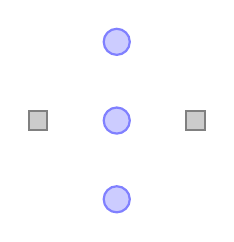
\begin{tikzpicture}[thick]
  \node at ( 0,2) [circle,draw=blue!50,fill=blue!20] {};
  \node at ( 0,1) [circle,draw=blue!50,fill=blue!20] {};
  \node at ( 0,0) [circle,draw=blue!50,fill=blue!20] {};
  \node at ( 1,1) [rectangle,draw=black!50,fill=black!20] {};
  \node at (-1,1) [rectangle,draw=black!50,fill=black!20] {};
\end{tikzpicture}
\end{codeexample}

% While this looks nicer in the picture, the code starts to get a bit ugly. Ideally, we would like our code to transport the message ``there are three places and two transitions'' and not so much which filling colors should be used.

虽然这在图片中看起来更好,但是代码开始变得有些难看。 理想情况下,我们希望代码传递``有三个库所和两个变迁''的消息,而不是要使用哪种填充颜色。

% To solve this problem, Hagen uses styles. He defines a style for places and another style for transitions:

为了解决此问题,哈根使用了样式。 他为库所定义了一种样式,为变迁定义了另一种样式:

%
\begin{codeexample}[]
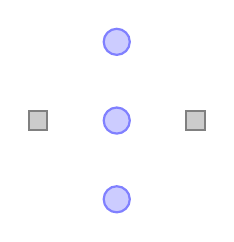
\begin{tikzpicture}
  [place/.style={circle,draw=blue!50,fill=blue!20,thick},
   transition/.style={rectangle,draw=black!50,fill=black!20,thick}]
  \node at ( 0,2) [place] {};
  \node at ( 0,1) [place] {};
  \node at ( 0,0) [place] {};
  \node at ( 1,1) [transition] {};
  \node at (-1,1) [transition] {};
\end{tikzpicture}
\end{codeexample}


% \subsection{Node Size}
\subsection{节点尺寸}

% Before Hagen starts naming and connecting the nodes, let us first make sure that the nodes get their final appearance. They are still too small. Indeed, Hagen wonders why they have any size at all, after all, the text is empty. The reason is that \tikzname\ automatically adds some space around the text. The amount is set using the option |inner sep|. So, to increase the size of the nodes, Hagen could write:

在哈根开始命名和连接节点之前,让我们首先确定节点具有最终外观。 它们还有点太小。 的确,哈根想知道为什么它们根本没有任何尺寸,毕竟文本是空的。 原因是\tikzname\ 会在文本周围自动添加一些空格。 空格的数量是使用选项 |inner sep| 设置的。 因此,为了增加节点的大小,哈根可以这样写:

%
\begin{codeexample}[]
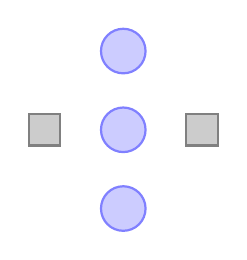
\begin{tikzpicture}
  [inner sep=2mm,
   place/.style={circle,draw=blue!50,fill=blue!20,thick},
   transition/.style={rectangle,draw=black!50,fill=black!20,thick}]
  \node at ( 0,2) [place] {};
  \node at ( 0,1) [place] {};
  \node at ( 0,0) [place] {};
  \node at ( 1,1) [transition] {};
  \node at (-1,1) [transition] {};
\end{tikzpicture}
\end{codeexample}

% However, this is not really the best way to achieve the desired effect. It is much better to use the |minimum size| option instead. This option allows Hagen to specify a minimum size that the node should have. If the node actually needs to be bigger because of a longer text, it will be larger, but if the text is empty, then the node will have |minimum size|. This option is also useful to ensure that several nodes containing different amounts of text have the same size. The options |minimum height| and |minimum width| allow you to specify the minimum height and width independently.

但是,这实际上并不是达到预期效果的最佳方法。 最好使用 |minimum size| 选项。 该选项允许哈根指定节点应具有的最小尺寸。 如果由于文本较长而实际上需要增大该节点,则该节点将变大,但是如果文本为空,则该节点将具有 |minimum size|。 这个选项对于确保包含不同长度的文本的几个节点具有相同的大小也很有用。 |minimum height| 和 |minimum width| 选项还允许您独立指定最小高度和最小宽度。

% So, what Hagen needs to do is to provide |minimum size| for the nodes. To be on the safe side, he also sets |inner sep=0pt|. This ensures that the nodes will really have size |minimum size| and not, for very small minimum sizes, the minimal size necessary to encompass the automatically added space.

因此,哈根需要做的就是给节点提供|minimum size|。 为了安全起见,他还设置了 |inner sep=0pt|。 这样可以确保节点真正具有|minimum size|。 而对于设置的非常小的的最小尺寸,节点并不是具有这个最小尺寸,而是包含自动添加的空间所需的最小尺寸。 

%
\begin{codeexample}[]
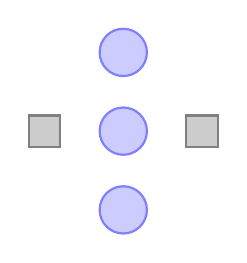
\begin{tikzpicture}
  [place/.style={circle,draw=blue!50,fill=blue!20,thick,
                 inner sep=0pt,minimum size=6mm},
   transition/.style={rectangle,draw=black!50,fill=black!20,thick,
                      inner sep=0pt,minimum size=4mm}]
  \node at ( 0,2) [place] {};
  \node at ( 0,1) [place] {};
  \node at ( 0,0) [place] {};
  \node at ( 1,1) [transition] {};
  \node at (-1,1) [transition] {};
\end{tikzpicture}
\end{codeexample}


% \subsection{Naming Nodes}
\subsection{节点命名}

% Hagen's next aim is to connect the nodes using arrows. This seems like a tricky business since the arrows should not start in the middle of the nodes, but somewhere on the border and Hagen would very much like to avoid computing these positions by hand.

哈根的下一个目标是使用箭头连接节点。 这似乎是一项棘手的工作,因为箭头不应从节点的中间开始,而是边界上的某个地方,哈根非常希望避免手动计算这些位置。

% Fortunately, \pgfname\ will perform all the necessary calculations for him. However, he first has to assign names to the nodes so that he can reference them later on. 

幸运的是,\pgfname\ 将为他执行所有必要的计算。 但是,他首先必须为节点分配名称,以便以后可以引用它们。

% There are two ways to name a node. The first is to use the |name=| option. The second method is to write the desired name in parentheses after the |node| operation. Hagen thinks that this second method seems strange, but he will soon change his opinion.

命名节点有两种方法。 第一种是使用 |name=| 选项。 第二种方法是在 |node| 操作之后的括号中写入节点的名称。哈根认为第二种方法似乎很奇怪,但是他很快就会改变看法。

%
\begin{codeexample}[setup code,hidden]
\tikzset{
    place/.style={circle,draw=blue!50,fill=blue!20,thick,
                  inner sep=0pt,minimum size=6mm},
    transition/.style={rectangle,draw=black!50,fill=black!20,thick,
                       inner sep=0pt,minimum size=4mm}
}
\end{codeexample}
%
\begin{codeexample}[]
% ... set up styles
\begin{tikzpicture}
  \node (waiting 1)      at ( 0,2) [place] {};
  \node (critical 1)     at ( 0,1) [place] {};
  \node (semaphore)      at ( 0,0) [place] {};
  \node (leave critical) at ( 1,1) [transition] {};
  \node (enter critical) at (-1,1) [transition] {};
\end{tikzpicture}
\end{codeexample}

% Hagen is pleased to note that the names help in understanding the code. Names for nodes can be pretty arbitrary, but they should not contain commas, periods, parentheses, colons, and some other special characters. However, they can contain underscores and hyphens.

哈根很高兴地注意到,这些名称有助于理解代码。 节点的名称可以是任意的,但它们不应包含逗号,句点,括号,冒号和其他一些特殊字符。 但是,它们可以包含下划线和连字符。

% The syntax for the |node| operation is quite liberal with respect to the order in which node names, the |at| specifier, and the options must come. Indeed, you can even have multiple option blocks between the |node| and the text in curly braces, they accumulate. You can rearrange them arbitrarily and perhaps the following might be preferable:

|node| 操作的语法在节点名称、|at| 和必须提供的选项的顺序方面是相当自由的。实际上,你甚至可以在 |node| 和花括号文本之间有多个选项块,它们会累积。你可以随意地重新排列它们,也许下面的方法更可取:

%
\begin{codeexample}[]
\begin{tikzpicture}
  \node[place]      (waiting 1)      at ( 0,2) {};
  \node[place]      (critical 1)     at ( 0,1) {};
  \node[place]      (semaphore)      at ( 0,0) {};
  \node[transition] (leave critical) at ( 1,1) {};
  \node[transition] (enter critical) at (-1,1) {};
\end{tikzpicture}
\end{codeexample}


% \subsection{Placing Nodes Using Relative Placement}
\subsection{使用相对位置放置节点}

% Although Hagen still wishes to connect the nodes, he first wishes to address another problem again: The placement of the nodes. Although he likes the |at| syntax, in this particular case he would prefer placing the nodes ``relative to each other''. So, Hagen would like to say that the |critical 1| node should be below the |waiting 1| node, wherever the |waiting 1| node might be. There are different ways of achieving this, but the nicest one in Hagen's case is the |below| option:

尽管哈根仍然希望连接节点,但他首先希望再次解决另一个问题:节点的放置。 尽管他喜欢 |at| 语法,在这种情况下,他宁愿将节点``彼此相对''地进行放置。 因此,哈根想说 |critical 1| 节点应在 |waiting 1| 节点的下方,无论 |waiting 1| 节点可能在哪个位置。 有多种方法可以实现此目的,但是在哈根的案例中,最好的方法是使用 |belloe| 选项:

%
\begin{codeexample}[preamble={\usetikzlibrary{positioning}}]
\begin{tikzpicture}
  \node[place]      (waiting)                            {};
  \node[place]      (critical)       [below=of waiting]  {};
  \node[place]      (semaphore)      [below=of critical] {};
  \node[transition] (leave critical) [right=of critical] {};
  \node[transition] (enter critical) [left=of critical]  {};
\end{tikzpicture}
\end{codeexample}

% With the |positioning| library loaded, when an option like |below| is followed by |of|, then the position of the node is shifted in such a manner that it is placed at the distance |node distance| in the specified direction of the given direction. The |node distance| is either the distance between the centers of the nodes (when the |on grid| option is set to true) or the distance between the borders (when the |on grid| option is set to false, which is the default).

加载 |positioning| 库后,当 |bellow| 选项后面跟着 |of| 时,则将节点的位置移动到指定方向,使其置于与指定节点的距离为 |node distance| 的位置。|node distance| 要么是节点中心之间的距离(当 |on grid| 选项被设置为true时),要么是边界之间的距离(当 |on grid| 选项被设置为false时,这是默认值)。

% Even though the above code has the same effect as the earlier code, Hagen can pass it to his colleagues who will be able to just read and understand it, perhaps without even having to see the picture.

即使上面的代码与早期的代码具有相同的效果,哈根仍可以将其传递给他的同事,他们甚至可以不必看图片就可以阅读和理解它。


% \subsection{Adding Labels Next to Nodes}
\subsection{在节点旁添加标签}

% Before we have a look at how Hagen can connect the nodes, let us add the capacity ``$s \le 3$'' to the bottom node. For this, two approaches are possible:

在查看哈根如何连接节点之前,让我们将容量``$s \le 3$''添加到底部节点。 为此,可以采用两种方法:

%
\begin{enumerate}
    % \item Hagen can just add a new node above the |north| anchor of the |semaphore| node.
    \item 哈根只需要在 |semaphore| 节点的 |north| 锚点上方添加一个新节点。
    %
\begin{codeexample}[preamble={\usetikzlibrary{positioning}}]
\begin{tikzpicture}
  \node[place]      (waiting)                            {};
  \node[place]      (critical)       [below=of waiting]  {};
  \node[place]      (semaphore)      [below=of critical] {};
  \node[transition] (leave critical) [right=of critical] {};
  \node[transition] (enter critical) [left=of critical]  {};

  \node [red,above] at (semaphore.north) {$s\le 3$};
\end{tikzpicture}
\end{codeexample}
        %
    % This is a general approach that will ``always work''.

    这是一种将``始终有效''的通用方法。

    % \item Hagen can use the special |label| option. This option is given to a |node| and it causes \emph{another} node to be added next to the node where the option is given. Here is the idea: When we construct the |semaphore| node, we wish to indicate that we want another node with the capacity above it. For this, we use the option |label=above:$s\le 3$|. This option is interpreted as follows: We want a node above the |semaphore| node and this node should read ``$s \le 3$''. Instead of |above| we could also use things like |below left| before the colon or a number like |60|.
    \item 哈根还可以使用特殊的 |label| 选项。 该选项被赋给 |node|, 使\emph{另一个}节点被添加到给出该选项的节点旁边。 这里是一个想法:当创建 |semaphore| 节点时,我们希望表明我们想要另一个位置高于它的节点。 为此,我们使用选项 |label=above:$s\le 3$|。 此选项的解释如下:我们希望在 |semaphore| 上方有一个节点,此节点应显示为``$s \le 3$''。 除了 |above| 我们还可以在冒号或在 |60| 之类的数字之前使用 |below left|。
    %
\begin{codeexample}[preamble={\usetikzlibrary{positioning}}]
\begin{tikzpicture}
  \node[place]      (waiting)                            {};
  \node[place]      (critical)       [below=of waiting]  {};
  \node[place]      (semaphore)      [below=of critical,
                                      label=above:$s\le3$] {};
  \node[transition] (leave critical) [right=of critical] {};
  \node[transition] (enter critical) [left=of critical]  {};
\end{tikzpicture}
\end{codeexample}
        %
    % It is also possible to give multiple |label| options, this causes multiple labels to be drawn.

    也可以给多个 |label| 选项,将会绘制多个标签。
    %
\begin{codeexample}[]
\tikz
  \node [circle,draw,label=60:$60^\circ$,label=below:$-90^\circ$] {my circle};
\end{codeexample}
        %
    % Hagen is not fully satisfied with the |label| option since the label is not red. To achieve this, he has two options: First, he can redefine the |every label| style. Second, he can add options to the label's node. These options are given following the |label=|, so he would write |label=[red]above:$s\le3$|. However, this does not quite work since \TeX\ thinks that the |]| closes the whole option list of the |semaphore| node. So, Hagen has to add braces and writes |label={[red]above:$s\le3$}|. Since this looks a bit ugly, Hagen decides to redefine the |every label| style.

    哈根对 |label| 选项并不完全满意,因为标签不是红色的。为了实现这一点,他有两个选择:首先,他可以重新定义 |every label| 的风格。其次,他可以向标签的节点中添加选项。这些选项是按照 |label=| 给出的,所以他在上面写 |label=[red]above:$s\le3$|。然而,这并不能完全工作,因为\TeX\ 认为 |]| 结束了 |semaphore| 节点的整个选项列表。因此,哈根必须添加括号这样使用 |label={[red]above:$s\le3$}|。由于这看起来有点丑,哈根决定重新定义 |every label| 风格。
        %
\begin{codeexample}[preamble={\usetikzlibrary{positioning}}]
\begin{tikzpicture}[every label/.style={red}]
  \node[place]      (waiting)                            {};
  \node[place]      (critical)       [below=of waiting]  {};
  \node[place]      (semaphore)      [below=of critical,
                                      label=above:$s\le3$] {};
  \node[transition] (leave critical) [right=of critical] {};
  \node[transition] (enter critical) [left=of critical]  {};
\end{tikzpicture}
\end{codeexample}
\end{enumerate}


% \subsection{Connecting Nodes}
\subsection{连接节点}

% It is now high time to connect the nodes. Let us start with something simple, namely with the straight line from |enter critical| to |critical|. We want this line to start at the right side of |enter critical| and to end at the left side of |critical|. For this, we can use the \emph{anchors} of the nodes. Every node defines a whole bunch of anchors that lie on its border or inside it. For example, the |center| anchor is at the center of the node, the |west| anchor is on the left of the node, and so on. To access the coordinate of a node, we use a coordinate that contains the node's name followed by a dot, followed by the anchor's name:

现在是连接节点的时候了。 让我们先从简单的事情开始,即从直线的 |enter critical| 到 |critical|。 我们希望此直线从 |enter critical| 的右侧开始,并在 | critical| 的左侧结束。 为此,我们可以使用节点的\emph{锚点}。 每个节点都定义了一大堆锚点,这些锚点位于其边界上或内部。 例如,|center| 锚点位于节点的中心,|west| 锚点位于节点的左侧,依此类推。 要访问节点的坐标,我们使用一个坐标,该坐标包含节点名称,后跟一句点,再后跟锚点名称:

%
\begin{codeexample}[preamble={\usetikzlibrary{positioning}}]
\begin{tikzpicture}
  \node[place]      (waiting)                            {};
  \node[place]      (critical)       [below=of waiting]  {};
  \node[place]      (semaphore)      [below=of critical] {};
  \node[transition] (leave critical) [right=of critical] {};
  \node[transition] (enter critical) [left=of critical]  {};
  \draw [->] (critical.west) -- (enter critical.east);
\end{tikzpicture}
\end{codeexample}

% Next, let us tackle the curve from |waiting| to |enter critical|. This can be specified using curves and controls:

接下来,让我们处理从 |waiting| 到 |enter critical| 的曲线。可以使用曲线和控件来指定:

%
\begin{codeexample}[preamble={\usetikzlibrary{positioning}}]
\begin{tikzpicture}
  \node[place]      (waiting)                            {};
  \node[place]      (critical)       [below=of waiting]  {};
  \node[place]      (semaphore)      [below=of critical] {};
  \node[transition] (leave critical) [right=of critical] {};
  \node[transition] (enter critical) [left=of critical]  {};
  \draw [->] (enter critical.east) -- (critical.west);
  \draw [->] (waiting.west) .. controls +(left:5mm) and +(up:5mm)
                            .. (enter critical.north);
\end{tikzpicture}
\end{codeexample}

% Hagen sees how he can now add all his edges, but the whole process seems a but awkward and not very flexible. Again, the code seems to obscure the structure of the graphic rather than showing it.

哈根看到了他现在如何添加他所有的边,但是整个过程看起来很笨拙,不是很灵活。再次,代码似乎使图形的结构变得晦涩,而不是展示图形是如何绘制而来的。

% So, let us start improving the code for the edges. First, Hagen can leave out the anchors:

因此,让我们开始改进边的代码。 首先,哈根可以省略锚点:

%
\begin{codeexample}[preamble={\usetikzlibrary{positioning}}]
\begin{tikzpicture}
  \node[place]      (waiting)                            {};
  \node[place]      (critical)       [below=of waiting]  {};
  \node[place]      (semaphore)      [below=of critical] {};
  \node[transition] (leave critical) [right=of critical] {};
  \node[transition] (enter critical) [left=of critical]  {};
  \draw [->] (enter critical) -- (critical);
  \draw [->] (waiting) .. controls +(left:8mm) and +(up:8mm)
                       .. (enter critical);
\end{tikzpicture}
\end{codeexample}

% Hagen is a bit surprised that this works. After all, how did \tikzname\ know that the line from |enter critical| to |critical| should actually start on the borders? Whenever \tikzname\ encounters a whole node name as a ``coordinate'', it tries to ``be smart'' about the anchor that it should choose for this node. Depending on what happens next, \tikzname\ will choose an anchor that lies on the border of the node on a line to the next coordinate or control point. The exact rules are a bit complex, but the chosen point will usually be correct -- and when it is not, Hagen can still specify the desired anchor by hand.

哈根有点惊讶,这是可行的。毕竟,\tikzname\ 怎么知道从 |enter critical| 到 |critical| 的直线实际上应该从边界开始呢?每当\tikzname\ 遇到作为``坐标''的整个节点名时,它就会尝试``“''聪明地''”''为该节点选择锚点。根据接下来发生的情况,\tikzname\ 将选择位于节点边界上的锚点,该锚点位于到下一个坐标或控制点的直线上。确切的规则有点复杂,但选择的点通常是正确的,如果不是这样,哈根仍然可以手工指定所需的锚点。

% Hagen would now like to simplify the curve operation somehow. It turns out that this can be accomplished using a special path operation: the |to| operation. This operation takes many options (you can even define new ones yourself). One pair of options is useful for Hagen: The pair |in| and |out|. These options take angles at which a curve should leave or reach the start or target coordinates. Without these options, a straight line is drawn:

哈根现在想以某种方式简化曲线操作。 事实证明,这可以使用特殊的路径操作来实现:|to| 操作。 此操作有很多选项(您甚至可以自己定义新选项)。 这组选项对哈根很有用:|in| 和 |out| 组。 这些选项采用曲线应离开或到达起始坐标或目标坐标的角度。如果没有这些选项,则会绘制一条直线:

%
\begin{codeexample}[preamble={\usetikzlibrary{positioning}}]
\begin{tikzpicture}
  \node[place]      (waiting)                            {};
  \node[place]      (critical)       [below=of waiting]  {};
  \node[place]      (semaphore)      [below=of critical] {};
  \node[transition] (leave critical) [right=of critical] {};
  \node[transition] (enter critical) [left=of critical]  {};
  \draw [->] (enter critical) to                 (critical);
  \draw [->] (waiting)        to [out=180,in=90] (enter critical);
\end{tikzpicture}
\end{codeexample}

% There is another option for the |to| operation, that is even better suited to Hagen's problem: The |bend right| option. This option also takes an angle, but this angle only specifies the angle by which the curve is bent to the right:

|to| 操作还有另一种选项,它甚至更适合于哈根的问题:|bend right| 选项。 此选项也需要一个角度,但是此角度仅指定曲线向右弯曲的角度:

%
\begin{codeexample}[preamble={\usetikzlibrary{positioning}}]
\begin{tikzpicture}
  \node[place]      (waiting)                            {};
  \node[place]      (critical)       [below=of waiting]  {};
  \node[place]      (semaphore)      [below=of critical] {};
  \node[transition] (leave critical) [right=of critical] {};
  \node[transition] (enter critical) [left=of critical]  {};
  \draw [->] (enter critical) to                 (critical);
  \draw [->] (waiting)        to [bend right=45] (enter critical);
  \draw [->] (enter critical) to [bend right=45] (semaphore);
\end{tikzpicture}
\end{codeexample}

% It is now time for Hagen to learn about yet another way of specifying edges: Using the |edge| path operation. This operation is very similar to the |to| operation, but there is one important difference: Like a node the edge generated by the |edge| operation is not part of the main path, but is added only later. This may not seem very important, but it has some nice consequences. For example, every edge can have its own arrow tips and its own color and so on and, still, all the edges can be given on the same path. This allows Hagen to write the following:

现在是时候让哈根学习指定边的另一种方法了:使用 |edge| 路径操作。 此操作与 |to| 非常相似。 操作,但是有一个重要的区别:与节点一样,|edge| 操作生成的边不是主路径的一部分,而是仅在以后添加。 这看似不太重要,但是会带来一些不错的效果。 例如,每条边可以有自己的箭头提示和颜色,依此类推,而且所有边都可以在同一路径上给出。 这使哈根可以编写以下内容:

%
\begin{codeexample}[preamble={\usetikzlibrary{positioning}}]
\begin{tikzpicture}
  \node[place]      (waiting)                            {};
  \node[place]      (critical)       [below=of waiting]  {};
  \node[place]      (semaphore)      [below=of critical] {};
  \node[transition] (leave critical) [right=of critical] {};
  \node[transition] (enter critical) [left=of critical]  {}
    edge [->]               (critical)
    edge [<-,bend left=45]  (waiting)
    edge [->,bend right=45] (semaphore);
\end{tikzpicture}
\end{codeexample}

% Each |edge| caused a new path to be constructed, consisting of a |to| between the node |enter critical| and the node following the |edge| command.

每个 |edge| 都会绘制一条新路径,每条路径的命令都由 |enter critical| 节点和 |edge| 命令之后的节点组成,节点之间采用 |to| 连接。

% The finishing touch is to introduce two styles |pre| and |post| and to use the |bend angle=45| option to set the bend angle once and for all:

最后要介绍的是 |pre| 和 |post| 两种样式,并使用|bend angle=45| 选项一劳永逸地设置弯曲角度:

%
\begin{codeexample}[preamble={\usetikzlibrary{arrows.meta,positioning}}]
% Styles place and transition as before
\begin{tikzpicture}
  [bend angle=45,
   pre/.style={<-,shorten <=1pt,>={Stealth[round]},semithick},
   post/.style={->,shorten >=1pt,>={Stealth[round]},semithick}]

  \node[place]      (waiting)                            {};
  \node[place]      (critical)       [below=of waiting]  {};
  \node[place]      (semaphore)      [below=of critical] {};

  \node[transition] (leave critical) [right=of critical] {}
    edge [pre]             (critical)
    edge [post,bend right] (waiting)
    edge [pre, bend left]  (semaphore);
  \node[transition] (enter critical) [left=of critical]  {}
    edge [post]            (critical)
    edge [pre, bend left]  (waiting)
    edge [post,bend right] (semaphore);
\end{tikzpicture}
\end{codeexample}


% \subsection{Adding Labels Next to Lines}
\subsection{在线旁添加标签}

% The next thing that Hagen needs to add is the ``$2$'' at the arcs. For this Hagen can use \tikzname's automatic node placement: By adding the option |auto|, \tikzname\ will position nodes on curves and lines in such a way that they are not on the curve but next to it. Adding |swap| will mirror the label with respect to the line. Here is a general example:

哈根接下来需要添加的是弧线上的``$2$''。 为此,哈根可以使用\tikzname 的自动节点放置:通过添加选项 |auto|,\tikzname\ 可以将节点定位在曲线和线上,使得它们不在曲线上而是位于曲线旁边。 添加 |swap| 将对该线的标签进行镜像。 这是一个一般示例:

%
% TODOsp: codeexamples: styles not needed here
\begin{codeexample}[]
\begin{tikzpicture}[auto,bend right]
  \node (a) at (0:1) {$0^\circ$};
  \node (b) at (120:1) {$120^\circ$};
  \node (c) at (240:1) {$240^\circ$};

  \draw (a) to node {1} node [swap] {1'} (b)
        (b) to node {2} node [swap] {2'} (c)
        (c) to node {3} node [swap] {3'} (a);
\end{tikzpicture}
\end{codeexample}

% What is happening here? The nodes are given somehow inside the |to| operation! When this is done, the node is placed on the middle of the curve or line created by the |to| operation. The |auto| option then causes the node to be moved in such a way that it does not lie on the curve, but next to it. In the example we provide even two nodes on each |to| operation.  For Hagen that |auto| option is not really necessary since the two ``2'' labels could also easily be placed ``by hand''. However, in a complicated plot with numerous edges automatic placement can be a blessing.

这里发生了什么?节点以某种方式在 |to| 操作中给定!完成此操作后,节点被放置在 |to| 操作创建的曲线或直线的中间。然后,|auto| 选项导致节点以这样一种方式进行移动,即它不在曲线上,而是在曲线旁边。在本例中,我们为每个 |to| 操作提供两个节点。对于哈根来说,|auto| 选项并不是真正必要的,因为两个``2''标签也可以很容易地``手动''放置。然而,在一个有许多边的复杂情形中,自动放置可能是一件好事。

%
\begin{codeexample}[
    preamble={\usetikzlibrary{arrows.meta,positioning}},
    pre={\tikzset{
    pre/.style={<-,shorten <=1pt,>={Stealth[round]},semithick},
    post/.style={->,shorten >=1pt,>={Stealth[round]},semithick},
}},
]
% Styles as before
\begin{tikzpicture}[bend angle=45]
  \node[place]      (waiting)                            {};
  \node[place]      (critical)       [below=of waiting]  {};
  \node[place]      (semaphore)      [below=of critical] {};

  \node[transition] (leave critical) [right=of critical] {}
    edge [pre]                                 (critical)
    edge [post,bend right] node[auto,swap] {2} (waiting)
    edge [pre, bend left]                      (semaphore);
  \node[transition] (enter critical) [left=of critical]  {}
    edge [post]                                (critical)
    edge [pre, bend left]                      (waiting)
    edge [post,bend right]                     (semaphore);
\end{tikzpicture}
\end{codeexample}
% TODOsp: codeexamples: styles and `positioning` are needed up to here


% \subsection{Adding the Snaked Line and Multi-Line Text}
\subsection{添加隐藏线和多行文本}

% With the node mechanism Hagen can now easily create the two Petri nets. What he is unsure of is how he can create the snaked line between the nets.

利用节点机制,哈根现在可以轻松创建两个Petri网络。 他不确定的是如何在网之间创建蛇形线。

% For this he can use a \emph{decoration}. To draw the snaked line, Hagen only needs to set the two options |decoration=snake| and |decorate| on the path. This causes all lines of the path to be replaced by snakes. It is also possible to use snakes only in certain parts of a path, but Hagen will not need this. 

为此,他可以使用\emph{decoration}库。 要绘制蛇形线,哈根只需要为路径设置两个选项 |decoration=snake| 和 |decorate|。 这将导致路径的所有线都被蛇形替换。 也可以仅在路径的某些部分使用蛇形,但是哈根不需要。

\begin{codeexample}[preamble={\usetikzlibrary{decorations.pathmorphing}}]
\begin{tikzpicture}
  \draw [->,decorate,decoration=snake] (0,0) -- (2,0);
\end{tikzpicture}
\end{codeexample}

% Well, that does not look quite right, yet. The problem is that the snake happens to end exactly at the position where the arrow begins. Fortunately, there is an option that helps here. Also, the snake should be a bit smaller, which can be influenced by even more options.

好吧,这看起来还不太正确。 问题是蛇形恰好在箭头开始的位置结束。 幸运的是,这里有一个选项可以帮助您。 同样,蛇形应该更小一些,这可能会受到更多选择的影响。

%
\begin{codeexample}[preamble={\usetikzlibrary{decorations.pathmorphing}}]
\begin{tikzpicture}
  \draw [->,decorate,
     decoration={snake,amplitude=.4mm,segment length=2mm,post length=1mm}]
    (0,0) -- (3,0);
\end{tikzpicture}
\end{codeexample}

% Now Hagen needs to add the text above the snake. This text is a bit challenging since it is a multi-line text. Hagen has two options for this: First, he can specify an |align=center| and then use the |\\| command to enforce the line breaks at the desired positions.

现在,哈根需要在蛇形上方添加文本。 该文本是多行文本,因此具有一定的挑战性。 哈根对此有两种选择:首先,他可以指定 |align=center|。 然后使用 |\\| 命令以在所需位置强制换行。

%
\begin{codeexample}[preamble={\usetikzlibrary{decorations.pathmorphing}}]
\begin{tikzpicture}
  \draw [->,decorate,
      decoration={snake,amplitude=.4mm,segment length=2mm,post length=1mm}]
    (0,0) -- (3,0)
    node [above,align=center,midway]
    {
      replacement of\\
      the \textcolor{red}{capacity}\\
      by \textcolor{red}{two places}
    };
\end{tikzpicture}
\end{codeexample}

% Instead of specifying the line breaks ``by hand'', Hagen can also specify a width for the text and let \TeX\ perform the line breaking for him:

哈根除了可以手动指定换行符之外,还可以为文本指定宽度并让\TeX\ 为他自动换行:

%
\begin{codeexample}[preamble={\usetikzlibrary{decorations.pathmorphing}}]
\begin{tikzpicture}
  \draw [->,decorate,
      decoration={snake,amplitude=.4mm,segment length=2mm,post length=1mm}]
    (0,0) -- (3,0)
    node [above,text width=3cm,align=center,midway]
    {
      replacement of the \textcolor{red}{capacity} by
      \textcolor{red}{two places}
    };
\end{tikzpicture}
\end{codeexample}


% \subsection{Using Layers: The Background Rectangles}
\subsection{使用图层:背景矩形}

% Hagen still needs to add the background rectangles. These are a bit tricky: Hagen would like to draw the rectangles \emph{after} the Petri nets are finished. The reason is that only then can he conveniently refer to the coordinates that make up the corners of the rectangle. If Hagen draws the rectangle first, then he needs to know the exact size of the Petri net -- which he does not.

哈根仍然需要添加背景矩形。 这些有点棘手:哈根希望在Petri网绘制完成\emph{之后}再绘制矩形。 原因是只有这样,他才能方便地得到矩形角点的坐标。如果哈根首先画出这个矩形,那么他需要知道Petri网的确切大小,但他并不知道。

% The solution is to use \emph{layers}. When the |backgrounds| library is loaded, Hagen can put parts of his picture inside a scope with the |on background layer| option. Then this part of the picture becomes part of the layer that is given as an argument to this environment. When the |{tikzpicture}| environment ends, the layers are put on top of each other, starting with the background layer. This causes everything drawn on the background layer to be behind the main text.

解决方案是使用\emph{图层}。|backgrounds| 库已加载,哈根可以将其图片的一部分放置在具有``背景层''的范围内。 然后,图片的该部分成为该环境的参数所指定的图层的一部分。 当 |{tikzpicture}| 在环境结束时,各层从背景层开始相互重叠。 这导致在背景层上绘制的所有内容都位于主文本的后面。

% The next tricky question is, how big should the rectangle be? Naturally, Hagen can compute the size ``by hand'' or using some clever observations concerning the $x$- and $y$-coordinates of the nodes, but it would be nicer to just have \tikzname\ compute a rectangle into which all the nodes ``fit''. For this, the |fit| library can be used. It defines the |fit| options, which, when given to a node, causes the node to be resized and shifted such that it exactly covers all the nodes and coordinates given as parameters to the |fit| option.

下一个棘手的问题是,矩形应该有多大? 当然,哈根可以``手工''计算大小,也可以使用一些聪明的方法来计算节点的$x$和$y$的坐标,但如果使用\tikzname\ 计算一个所有节点都适合的矩形会更好。 为此,可以使用 |fit| 库。它定义了 |fit| 选项,当将该选项提供给节点时,将对该节点的大小进行调整和移动,以便准确地覆盖作为 |fit| 选项参数提供的所有节点和坐标。

%
% TODOsp: codeexamples: redo/add styles starting from here
\begin{codeexample}[
    preamble={\usetikzlibrary{arrows.meta,backgrounds,fit,positioning}},
    pre={\tikzset{
    pre/.style={<-,shorten <=1pt,>={Stealth[round]},semithick},
    post/.style={->,shorten >=1pt,>={Stealth[round]},semithick},
}},
]
% Styles as before
\begin{tikzpicture}[bend angle=45]
  \node[place]      (waiting)                            {};
  \node[place]      (critical)       [below=of waiting]  {};
  \node[place]      (semaphore)      [below=of critical] {};

  \node[transition] (leave critical) [right=of critical] {}
    edge [pre]                                 (critical)
    edge [post,bend right] node[auto,swap] {2} (waiting)
    edge [pre, bend left]                      (semaphore);
  \node[transition] (enter critical) [left=of critical]  {}
    edge [post]                                (critical)
    edge [pre, bend left]                      (waiting)
    edge [post,bend right]                     (semaphore);

  \begin{scope}[on background layer]
    \node [fill=black!30,fit=(waiting) (critical) (semaphore)
             (leave critical) (enter critical)] {};
  \end{scope}
\end{tikzpicture}
\end{codeexample}


% \subsection{The Complete Code}
\subsection{完整的代码}

% Hagen has now finally put everything together. Only then does he learn that there is already a library for drawing Petri nets! It turns out that this library mainly provides the same definitions as Hagen did. For example, it defines a |place| style in a similar way as Hagen did. Adjusting the code so that it uses the library shortens Hagen code a bit, as shown in the following.

哈根现在终于把所有东西都放在一起了。 这时,他才知道已经有了一个绘制Petri网的库! 事实证明,该库主要提供与哈根相同的定义。 例如,它定义了 |place|,与哈根类似。 调整代码以便使用该库,缩短了哈根的代码,如下所示。

%First, Hagen needs less style definitions, but he still needs to specify the colors of places and transitions.

首先,哈根需要较少的样式定义,但他仍然需要指定库所和变迁的颜色。

%
\begin{codeexample}[code only]
\begin{tikzpicture}
  [node distance=1.3cm,on grid,>={Stealth[round]},bend angle=45,auto,
   every place/.style=     {minimum size=6mm,thick,draw=blue!75,fill=blue!20},
   every transition/.style={thick,draw=black!75,fill=black!20},
   red place/.style=       {place,draw=red!75,fill=red!20},
   every label/.style=     {red}]
\end{codeexample}

% Now comes the code for the nets:

现在我们得到了网络的代码:

%
\ifpgfmanualexternalize\tikzexternaldisable\fi
\begin{codeexample}[
    preamble={\usetikzlibrary{arrows.meta,petri,positioning}},
    pre={\tikzset{
    every place/.style={minimum size=6mm,thick,draw=blue!75,fill=blue!20},
    every transition/.style={thick,draw=black!75,fill=black!20},
    every label/.style={red},
    every picture/.style={on grid,node distance=1.3cm,>={Stealth[round]},bend angle=45,auto},
}%
\begin{tikzpicture}},
    post={\end{tikzpicture}},
]
   \node [place,tokens=1] (w1)                                    {};
   \node [place]          (c1) [below=of w1]                      {};
   \node [place]          (s)  [below=of c1,label=above:$s\le 3$] {};
   \node [place]          (c2) [below=of s]                       {};
   \node [place,tokens=1] (w2) [below=of c2]                      {};

   \node [transition] (e1) [left=of c1] {}
     edge [pre,bend left]                  (w1)
     edge [post,bend right]                (s)
     edge [post]                           (c1);
   \node [transition] (e2) [left=of c2] {}
     edge [pre,bend right]                 (w2)
     edge [post,bend left]                 (s)
     edge [post]                           (c2);
   \node [transition] (l1) [right=of c1] {}
     edge [pre]                            (c1)
     edge [pre,bend left]                  (s)
     edge [post,bend right] node[swap] {2} (w1);
   \node [transition] (l2) [right=of c2] {}
     edge [pre]                            (c2)
     edge [pre,bend right]                 (s)
     edge [post,bend left]  node {2}       (w2);
\end{codeexample}

\ifpgfmanualexternalize\tikzexternaldisable\fi
\begin{codeexample}[
    preamble={\usetikzlibrary{arrows.meta,petri,positioning}},
    pre={\tikzset{
    every place/.style={minimum size=6mm,thick,draw=blue!75,fill=blue!20},
    every transition/.style={thick,draw=black!75,fill=black!20},
    red place/.style=  {place,draw=red!75,fill=red!20},
    every label/.style={red},
    every picture/.style={on grid,node distance=1.3cm,>={Stealth[round]},bend angle=45,auto},
}%
\begin{tikzpicture}},
    post={\end{tikzpicture}},
]
  \begin{scope}[xshift=6cm]
    \node [place,tokens=1]     (w1')                            {};
    \node [place]              (c1') [below=of w1']             {};
    \node [red place]          (s1') [below=of c1',xshift=-5mm]
            [label=left:$s$]                                    {};
    \node [red place,tokens=3] (s2') [below=of c1',xshift=5mm]
            [label=right:$\bar s$]                              {};
    \node [place]              (c2') [below=of s1',xshift=5mm]  {};
    \node [place,tokens=1]     (w2') [below=of c2']             {};

    \node [transition] (e1') [left=of c1'] {}
      edge [pre,bend left]                  (w1')
      edge [post]                           (s1')
      edge [pre]                            (s2')
      edge [post]                           (c1');
    \node [transition] (e2') [left=of c2'] {}
      edge [pre,bend right]                 (w2')
      edge [post]                           (s1')
      edge [pre]                            (s2')
      edge [post]                           (c2');
    \node [transition] (l1') [right=of c1'] {}
      edge [pre]                            (c1')
      edge [pre]                            (s1')
      edge [post]                           (s2')
      edge [post,bend right] node[swap] {2} (w1');
    \node [transition] (l2') [right=of c2'] {}
      edge [pre]                            (c2')
      edge [pre]                            (s1')
      edge [post]                           (s2')
      edge [post,bend left]  node {2}       (w2');
  \end{scope}
\end{codeexample}

% The code for the background and the snake is the following:

背景和蛇形的代码如下:

%
\begin{codeexample}[code only]
  \begin{scope}[on background layer]
    \node (r1) [fill=black!10,rounded corners,fit=(w1)(w2)(e1)(e2)(l1)(l2)] {};
    \node (r2) [fill=black!10,rounded corners,fit=(w1')(w2')(e1')(e2')(l1')(l2')] {};
  \end{scope}

  \draw [shorten >=1mm,->,thick,decorate,
         decoration={snake,amplitude=.4mm,segment length=2mm,
                     pre=moveto,pre length=1mm,post length=2mm}]
    (r1) -- (r2) node [above=1mm,midway,text width=3cm,align=center]
      {replacement of the \textcolor{red}{capacity} by \textcolor{red}{two places}};
\end{tikzpicture}
\end{codeexample}

% -----------------------------------------------------------------------------
% TODOsp: codeexamples: This is needed because -- unlike I thought --
%         `setup code is remembered also outside this file. Thus the changed
%         style of `place` and `transition` are "remembered" in
%         <pgfmanual-en-library-petri.tex>
\begin{codeexample}[setup code,hidden]
% from <tikzlibrarypetri.code.tex>
\tikzset{
    place/.style={circle,draw,inner sep=0pt,minimum size=5ex,every place},
    transition/.style={rectangle,draw,inner sep=0pt,minimum size=4mm,every transition},
}
\end{codeexample}
% -----------------------------------------------------------------------------

\clearpage
% Copyright 2019 by Till Tantau
%
% This file may be distributed and/or modified
%
% 1. under the LaTeX Project Public License and/or
% 2. under the GNU Free Documentation License.
%
% See the file doc/generic/pgf/licenses/LICENSE for more details.


% \section{Tutorial: Euclid's Amber Version of the \emph{Elements}}
\section{教程:欧几里得的琥珀版本的\emph{几何原本}}

% In this third tutorial we have a look at how \tikzname\ can be used to draw geometric constructions.

在第三个教程中,我们将了解如何使用\tikzname\ 绘制几何构造。

% Euclid is currently quite busy writing his new book series, whose working title is ``Elements'' (Euclid is not quite sure whether this title will convey the message of the series to future generations correctly, but he intends to change the title before it goes to the publisher). Up to know, he wrote down his text and graphics on papyrus, but his publisher suddenly insists that he must submit in electronic form. Euclid tries to argue with the publisher that electronics will only be discovered thousands of years later, but the publisher informs him that the use of papyrus is no longer cutting edge technology and Euclid will just have to keep up with modern tools.

欧几里德(Euclid)目前正忙于撰写他的新书系列,其标题是``几何原本''(欧克利德不确定该标题是否会正确地向后人传达该系列的信息,但他打算在它交给出版商之前更改书名)。 据他所知,他在纸莎草纸上写下了文字和图形,但是他的出版商突然坚持要求他必须以电子形式提交。 欧几里得试图与出版商争辩,电子技术只会在数千年后才被发现,但是出版商告诉他,纸莎草纸的使用不再是尖端技术,欧几里得将不得不跟上现代工具的发展。

% Slightly disgruntled, Euclid starts converting his papyrus entitled ``Book I, Proposition I'' to an amber version.

欧几里得有些不满,开始将名为``书I,命题I''的纸莎草纸改成琥珀版本。


% \subsection{Book I, Proposition I}
\subsection{书I,命题I}

% The drawing on his papyrus looks like this:\footnote{The text is taken from the wonderful interactive version of Euclid's Elements by David E. Joyce, to be found on his website at Clark University.} 

他的纸莎草纸上的图形看起来像这样:\footnote{该文本摘自David E. Joyce的Euclid's Elements精彩互动版本,可在他在Clark University的网站上找到。}

\bigskip
\noindent
\begin{tikzpicture}[thick,help lines/.style={thin,draw=black!50}]
  \pgfmathsetseed{1}
  \def\A{\textcolor{input}{$A$}}
  \def\B{\textcolor{input}{$B$}}
  \def\C{\textcolor{output}{$C$}}
  \def\D{$D$}
  \def\E{$E$}

  \colorlet{input}{blue!80!black}
  \colorlet{output}{red!70!black}
  \colorlet{triangle}{orange}

  \coordinate [label=left:\A]
    (A) at ($ (0,0) + .1*(rand,rand) $);
  \coordinate [label=right:\B]
    (B) at ($ (1.25,0.25) + .1*(rand,rand) $);

  \draw [input] (A) -- (B);

  \node [name path=D,help lines,draw,label=left:\D] (D) at (A) [circle through=(B)] {};
  \node [name path=E,help lines,draw,label=right:\E] (E) at (B) [circle through=(A)] {};

  \path [name intersections={of=D and E,by={[label=above:\C]C}}];

  \draw [output] (A) -- (C);
  \draw [output] (B) -- (C);

  \foreach \point in {A,B,C}
    \fill [black,opacity=.5] (\point) circle (2pt);

  \begin{pgfonlayer}{background}
    \fill[triangle!80] (A) -- (C) -- (B) -- cycle;
  \end{pgfonlayer}

  \node [below right,text width=10cm,align=justify] at (4,3)
  {
    \small
    \textbf{Proposition I}\par
    \emph{To construct an \textcolor{triangle}{equilateral triangle}
      on a given \textcolor{input}{finite straight line}.}
    \par
    \vskip1em
    Let \A\B\ be the given \textcolor{input}{finite straight line}. It is required to construct an \textcolor{triangle}{equilateral triangle} on the \textcolor{input}{straight line}~\A\B.

    Describe the circle \B\C\D\ with center~\A\ and radius \A\B. Again describe the circle \A\C\E\ with center~\B\ and radius \B\A. Join the \textcolor{output}{straight lines} \C\A\ and \C\B\ from the point~\C\ at which the circles cut one another to the points~\A\ and~\B.

    Now, since the point~\A\ is the center of the circle \C\D\B, therefore \A\C\ equals \A\B. Again, since the point \B\ is the center of the circle \C\A\E, therefore \B\C\ equals \B\A. But \A\C\ was proved equal to \A\B, therefore each of the straight lines \A\C\ and \B\C\ equals \A\B. And     things which equal the same thing also equal one another, therefore \A\C\ also equals \B\C. Therefore the three straight lines \A\C, \A\B, and \B\C\ equal one another. Therefore the \textcolor{triangle}{triangle} \A\B\C\ is equilateral, and it has been  constructed on the given finite \textcolor{input}{straight line}~\A\B.
  };
\end{tikzpicture}
\bigskip

% Let us have a look at how Euclid can turn this into \tikzname\ code.

让我们看看欧几里得如何将其转换为\tikzname\ 代码。


% \subsubsection{Setting up the Environment}
\subsubsection{配置环境}

% As in the previous tutorials, Euclid needs to load \tikzname, together with some libraries. These libraries are |calc|, |intersections|, |through|, and |backgrounds|. Depending on which format he uses, Euclid would use one of the following in the preamble:

与以前的教程一样,欧几里得需要加载\tikzname 以及一些库。 这些库是包括 |calc|、|intersections|、|through| 和 | backgrounds|。 根据他使用的格式,欧几里得将在序言中使用以下其中之一:

%
\begin{codeexample}[code only]
% For LaTeX:
\usepackage{tikz}
\usetikzlibrary{calc,intersections,through,backgrounds}
\end{codeexample}

\begin{codeexample}[code only]
% For plain TeX:
\input tikz.tex
\usetikzlibrary{calc,intersections,through,backgrounds}
\end{codeexample}

\begin{codeexample}[code only]
% For ConTeXt:
\usemodule[tikz]
\usetikzlibrary[calc,intersections,through,backgrounds]
\end{codeexample}


%\subsubsection{The Line \emph{AB}}
\subsubsection{线段\emph{AB}}

% The first part of the picture that Euclid wishes to draw is the line $AB$. That is easy enough, something like |\draw (0,0) -- (2,1);| might do. However, Euclid does not wish to reference the two points $A$ and $B$ as $(0,0)$ and $(2,1)$ subsequently. Rather, he wishes to just write |A| and |B|. Indeed, the whole point of his book is that the points $A$ and $B$ can be arbitrary and all other points (like $C$) are constructed in terms of their positions. It would not do if Euclid were to write down the coordinates of $C$ explicitly.

欧几里得希望绘制图片的第一部分是$AB$线段。 这很容易,像 |\draw (0,0) -- (2,1);| 就可以做到。但是,欧几里得不希望随后将两个点$A$和$B$分别称为$(0,0)$和$(2,1)$。 相反,他希望只写 |A| 和 |B|,确实,他的书的要点是$A$和$B$点可以是任意的,其他所有点(如$C$)都是根据其位置构造的。如果欧几里得明确地写下$C$的坐标,它就不会这样做了。{\color{red}\ref{error}}

% So, Euclid starts with defining two coordinates using the |\coordinate| command:

因此,欧几里得从使用 |\coordinate| 命令定义两个坐标开始:

%
\begin{codeexample}[]
\begin{tikzpicture}
  \coordinate (A) at (0,0);
  \coordinate (B) at (1.25,0.25);

  \draw[blue] (A) -- (B);
\end{tikzpicture}
\end{codeexample}

% That was easy enough. What is missing at this point are the labels for the coordinates. Euclid does not want them \emph{on} the points, but next to them. He decides to use the |label| option:

这已经足够简单。此时缺少的是坐标的标签。 欧几里得不希望它们在这些坐标点\emph{上},而是在坐标点旁边。 他决定使用 |label| 选项:

%
\begin{codeexample}[]
\begin{tikzpicture}
  \coordinate [label=left:\textcolor{blue}{$A$}]  (A) at (0,0);
  \coordinate [label=right:\textcolor{blue}{$B$}] (B) at (1.25,0.25);

  \draw[blue] (A) -- (B);
\end{tikzpicture}
\end{codeexample}

% At this point, Euclid decides that it would be even nicer if the points $A$ and $B$ were in some sense ``random''. Then, neither Euclid nor the reader can make the mistake of taking ``anything for granted'' concerning these position of these points. Euclid is pleased to learn that there is a |rand| function in \tikzname\ that does exactly what he needs: It produces a number between $-1$ and $1$. Since \tikzname\ can do a bit of math, Euclid can change the coordinates of the points as follows:

在这一点上,欧几里得认为如果点$A$和$B$在某种意义上是``随机的'',那就更好了。 这样,无论是欧几里德还是读者都不会犯错误,认为这些点的位置是“理所当然的”。 欧几里得很高兴得知\tikzname\ 中的 |rand| 函数完全满足他的需要:它产生介于$-1$和$1$之间的数字。 由于\tikzname\ 可以进行一些数学运算,因此欧几里得可以如下更改点的坐标:

%
\begin{codeexample}[code only]
\coordinate [...] (A) at (0+0.1*rand,0+0.1*rand);
\coordinate [...] (B) at (1.25+0.1*rand,0.25+0.1*rand);
\end{codeexample}

% This works fine. However, Euclid is not quite satisfied since he would prefer that the ``main coordinates'' $(0,0)$ and $(1.25,0.25)$ are ``kept separate'' from the perturbation $0.1(\mathit{rand},\mathit{rand})$. This means, he would like to specify that coordinate $A$ as ``the point that is at $(0,0)$ plus one tenth of the vector  $(\mathit{rand},\mathit{rand})$''.

这确实很好。 但是,欧几里得并不十分满意,因为他希望``主坐标''$(0,0)$和$(1.25,0.25)$与扰动$0.1(\mathit{rand},\mathit{rand})$``保持分离''。 这意味着,他想将坐标$A$指定为``在$(0,0)$上加上向量$(\mathit{rand},\mathit{rand})$的十分之一''。

% It turns out that the |calc| library allows him to do exactly this kind of computation. When this library is loaded, you can use special coordinates that start with |($| and end with |$)| rather than just |(| and~|)|. Inside these special coordinates you can give a linear combination of coordinates. (Note that the dollar signs are only intended to signal that a ``computation'' is going on; no mathematical typesetting is done.)

事实证明 |calc| 库允许他精确地进行这种计算。 加载此库后,可以使用以 |($| 开始以及以 |$)| 结束的特殊坐标,而不只是 |(| 和 |)|。 在这些特殊坐标内,您可以给出坐标的线性组合。 (请注意,美元符号仅用于表示正在进行``计算'';不进行数学排版。)


% The new code for the coordinates is the following:

坐标新的代码如下:

%
\begin{codeexample}[code only]
\coordinate [...] (A) at ($ (0,0) + .1*(rand,rand) $);
\coordinate [...] (B) at ($ (1.25,0.25) + .1*(rand,rand) $);
\end{codeexample}

% Note that if a coordinate in such a computation has a factor (like |.1|), you must place a |*| directly before the opening parenthesis of the coordinate. You can nest such computations.

请注意,如果此类计算中的坐标有一个乘数(例如|.1|),则必须直接在坐标的圆括号之前放置|*|。 您可以嵌套进行这样的计算。


% \subsubsection{The Circle Around \emph{A}}
\subsubsection{以点\emph{A}为圆心的圆}

% The first tricky construction is the circle around $A$. We will see later how to do this in a very simple manner, but first let us do it the ``hard'' way.

第一个棘手的结构是以点$A$为圆心的圆。 稍后我们将看到如何以非常简单的方式执行此操作,但首先让我们以一种更``困难''方式执行此操作。

% The idea is the following: We draw a circle around the point $A$ whose radius is given by the length of the line $AB$. The difficulty lies in computing the length of this line.

想法如下:我们在点$A$周围画一个圆,其半径由线$AB$的长度给定。 困难在于计算这条线的长度。

% Two ideas ``nearly'' solve this problem: First, we can write |($ (A) - (B) $)| for the vector that is the difference between $A$ and~$B$. All we need is the length of this vector. Second, given two numbers $x$ and $y$, one can write |veclen(|$x$|,|$y$|)| inside a mathematical expression. This gives the value $\sqrt{x^2+y^2}$, which is exactly the desired length.

有两种``差不多''可以解决这个问题的想法:首先,我们可以说 |($ (A) - (B) $)| 是对于$A$和$B$之差的向量。 我们需要的只是该向量的长度。 第二,给定两个数字$x$和$y$,可以在数学表达式中使用 |veclen(|$x$|,|$y$|)|。 该表达式的值为$\sqrt{x^2+y^2}$,恰好是所需的长度。

% The only remaining problem is to access the $x$- and $y$-coordinate of the vector~$AB$. For this, we need a new concept: the \emph{let operation}. A let operation can be given anywhere on a path where a normal path operation like a line-to or a move-to is expected. The effect of a let operation is to evaluate some coordinates and to assign the results to special macros. These macros make it easy to access the $x$- and $y$-coordinates of the coordinates.


唯一剩下的问题是访问向量$AB$的$x$和$y$坐标。为此,我们需要一个新概念:\emph{let操作}。 let操作可以在路径上的任何位置进行,在这些位置可以进行常规的路径操作(如line-to或move-to)。let操作的作用是计算一些坐标,并将结果分配给特殊的宏。这些宏可以方便地访问坐标点的$x$和$y$坐标。

% Euclid would write the following:

欧几里得将编写以下内容:

%
\begin{codeexample}[preamble={\usetikzlibrary{calc}}]
\begin{tikzpicture}
  \coordinate [label=left:$A$]  (A) at (0,0);
  \coordinate [label=right:$B$] (B) at (1.25,0.25);
  \draw (A) -- (B);

  \draw (A) let
              \p1 = ($ (B) - (A) $)
            in
              circle ({veclen(\x1,\y1)});
\end{tikzpicture}
\end{codeexample}

% Each assignment in a let operation starts with |\p|, usually followed by a \meta{digit}. Then comes an equal sign and a coordinate. The coordinate is evaluated and the result is stored internally. From then on you can use the following expressions:

let操作中的每个赋值都以 |\p| 开始,通常后跟一个 \meta{数字},然后是等号和坐标。坐标将被计算,结果被存储在内部。之后你可以使用下面的表达方式:

%
\begin{enumerate}
    % \item |\x|\meta{digit} yields the $x$-coordinate of the resulting point.
    \item |\x|\meta{数字} 产生指定点的$x$坐标。
    % \item |\y|\meta{digit} yields the $y$-coordinate of the resulting point.
    \item |\y|\meta{数字} 产生指定点的$x$坐标。
    % \item |\p|\meta{digit} yields the same as |\x|\meta{digit}|,\y|\meta{digit}.
    \item |\p|\meta{数字} 产生与 |\x|\meta{数字}|,\y|\meta{数字} 相同的结果。
\end{enumerate}
%
% You can have multiple assignments in a let operation, just separate them with commas. In later assignments you can already use the results of earlier assignments.
%
在let操作中可以有多个赋值,只需用逗号分隔即可。 在以后的赋值中,您已经可以使用以前的赋值的结果。

% Note that |\p1| is not a coordinate in the usual sense. Rather, it just expands to a string like |10pt,20pt|. So, you cannot write, for instance, |(\p1.center)| since this would just expand to |(10pt,20pt.center)|, which makes no sense.

注意 |\p1| 不是通常意义上的坐标。相反,它只是扩展为一个字符串,如 |10pt,20pt|。例如,你不能写 |(\p1.center)| 因为它会扩展到 |(10pt,20pt.center)|,这没有意义。

% Next, we want to draw both circles at the same time. Each time the radius is |veclen(\x1,\y1)|. It seems natural to compute this radius only once. For this, we can also use a let operation: Instead of writing |\p1 = ...|, we write |\n2 = ...|. Here, ``n'' stands for ``number'' (while ``p'' stands for ``point''). The assignment of a number should be followed by a number in curly braces.

接下来,我们想要同时画两个圆。每个圆半径是 |veclen(\x1,\y1)|。只计算一次半径似乎很自然。为此,我们还可以使用let操作:他使用 |\n2 = ...| 代替 |\p1 = ...| 。这里,``n''代表``数字''(而``p''代表``点'')。数字的赋值后面应该跟一个用花括号括起来的数字。

%
\begin{codeexample}[preamble={\usetikzlibrary{calc}}]
\begin{tikzpicture}
  \coordinate [label=left:$A$]  (A) at (0,0);
  \coordinate [label=right:$B$] (B) at (1.25,0.25);
  \draw (A) -- (B);

  \draw let \p1 = ($ (B) - (A) $),
            \n2 = {veclen(\x1,\y1)}
        in
          (A) circle (\n2)
          (B) circle (\n2);
\end{tikzpicture}
\end{codeexample}
%
% In the above example, you may wonder, what |\n1| would yield? The answer is that it would be undefined -- the |\p|, |\x|, and |\y| macros refer to the same logical point, while the |\n| macro has ``its own namespace''. We could even have replaced |\n2| in the example by |\n1| and it would still work. Indeed, the digits following these macros are just normal \TeX\ parameters. We could also use a longer name, but then we have to use curly braces:

在上面的例子中,您可能想知道 |\n1| 会产生什么?答案是它将是未定义的,|\p|, |\x|,和 |\y| 宏引用相同的逻辑坐标点,而 |\n| 宏有''它自己的名称空间"。我们甚至可以把例子中的 |\n2| 替换成 |\n1| 而且仍然工作正常。实际上,这些宏后面的数字只是普通的\TeX\ 参数。我们也可以使用更长的名字,但我们必须使用花括号:

%
\begin{codeexample}[preamble={\usetikzlibrary{calc}}]
\begin{tikzpicture}
  \coordinate [label=left:$A$]  (A) at (0,0);
  \coordinate [label=right:$B$] (B) at (1.25,0.25);
  \draw (A) -- (B);

  \draw let \p1        = ($ (B) - (A) $),
            \n{radius} = {veclen(\x1,\y1)}
        in
          (A) circle (\n{radius})
          (B) circle (\n{radius});
\end{tikzpicture}
\end{codeexample}

% At the beginning of this section it was promised that there is an easier way to create the desired circle. The trick is to use the |through| library. As the name suggests, it contains code for creating shapes that go through a given point.

在本节的开始,我们承诺有一种更简单的方法来创建想要的圆。诀窍是通过使用|through| 库。顾名思义,它包含用于创建经过给定点的形状的代码。

% The option that we are looking for is |circle through|. This option is given to a \emph{node} and has the following effects: First, it causes the node's inner and outer separations to be set to zero. Then it sets the shape of the node to |circle|. Finally, it sets the radius of the node such that it goes through the parameter given to |circle through|. This radius is computed in essentially the same way as above.

我们需要的选项是 |circle through|。将此选项提供给\emph{节点}并具有以下效果:首先,它将使节点的内部和外部的间隔设置为零。然后它将节点的形状设置为 |circle|。最后,它设置节点的半径,使其通过给定的 |circle through|。这个半径的计算方法和上面一样。

%
\begin{codeexample}[preamble={\usetikzlibrary{through}}]
\begin{tikzpicture}
  \coordinate [label=left:$A$]  (A) at (0,0);
  \coordinate [label=right:$B$] (B) at (1.25,0.25);
  \draw (A) -- (B);

  \node [draw,circle through=(B),label=left:$D$] at (A) {};
\end{tikzpicture}
\end{codeexample}


% \subsubsection{The Intersection of the Circles}
\subsubsection{圆的交集}

% Euclid can now draw the line and the circles. The final problem is to compute the intersection of the two circles. This computation is a bit involved if you want to do it ``by hand''. Fortunately, the |intersections| library allows us to compute the intersection of arbitrary paths.

欧几里得现在可以画线段和圆了。最后一个问题是计算两个圆的交点。如果你想手工做的话,这个计算有点复杂。幸运的是,|intersections| 库允许我们计算任意路径的交集。

% The idea is simple: First, you ``name'' two paths using the |name path| option. Then, at some later point, you can use the option |name intersections|, which creates coordinates called |intersection-1|, |intersection-2|, and so on at all intersections of the paths. Euclid assigns the names |D| and |E| to the paths of the two circles (which happen to be the same names as the nodes themselves, but nodes and their paths live in different ``namespaces'').

其思想很简单:首先,使用|name path|选项给两条路径``命名''。然后,在以后的某个时候,您可以使用名称为 |name intersections| 选项,它在路径的所有交点上创建名为 |intersec-1|、|intersec-2| 的坐标,以此类推。欧几里德将名称 |D| 和 |E| 分配给两个圆的路径(这两个圆恰好与节点本身的名称相同,但节点及其路径位于不同的``名称空间''中)。

%
\begin{codeexample}[preamble={\usetikzlibrary{intersections,through}}]
\begin{tikzpicture}
  \coordinate [label=left:$A$]  (A) at (0,0);
  \coordinate [label=right:$B$] (B) at (1.25,0.25);
  \draw (A) -- (B);

  \node (D) [name path=D,draw,circle through=(B),label=left:$D$]  at (A) {};
  \node (E) [name path=E,draw,circle through=(A),label=right:$E$] at (B) {};

  % Name the coordinates, but do not draw anything:
  \path [name intersections={of=D and E}];

  \coordinate [label=above:$C$] (C) at (intersection-1);

  \draw [red] (A) -- (C);
  \draw [red] (B) -- (C);
\end{tikzpicture}
\end{codeexample}

% It turns out that this can be further shortened: The |name intersections| takes an optional argument |by|, which lets you specify names for the coordinates and options for them. This creates more compact code. Although Euclid does not need it for the current picture, it is just a small step to computing the bisection of the line $AB$:

事实证明,这个过程可以进一步缩减:|name intersections| 接受一个可选参数 |by|,它允许您为坐标指定名称和选项。这将创建更紧凑的代码。虽然欧几里得在现在的图中不需要它,但它只是计算直线AB的等分线的一个小步骤:

%
\begin{codeexample}[preamble={\usetikzlibrary{intersections,through}}]
\begin{tikzpicture}
  \coordinate [label=left:$A$]  (A) at (0,0);
  \coordinate [label=right:$B$] (B) at (1.25,0.25);
  \draw [name path=A--B] (A) -- (B);

  \node (D) [name path=D,draw,circle through=(B),label=left:$D$]  at (A) {};
  \node (E) [name path=E,draw,circle through=(A),label=right:$E$] at (B) {};

  \path [name intersections={of=D and E, by={[label=above:$C$]C, [label=below:$C'$]C'}}];

  \draw [name path=C--C',red] (C) -- (C');

  \path [name intersections={of=A--B and C--C',by=F}];
  \node [fill=red,inner sep=1pt,label=-45:$F$] at (F) {};
\end{tikzpicture}
\end{codeexample}


% \subsubsection{The Complete Code}
\subsubsection{完整代码}

% Back to Euclid's code. He introduces a few macros to make life simpler, like a |\A| macro for typesetting a blue $A$. He also uses the |background| layer for drawing the triangle behind everything at the end.

回到欧几里得的代码。他引入了一些宏来简化工作,比如用于排版蓝色的$A$的 |\A| 宏。他还使用了 |background| 层来绘制最后所有东西后面的三角形。

%
\begin{codeexample}[pre={\pgfmathsetseed{1}},preamble={\usetikzlibrary{backgrounds,calc,intersections,through}}]
\begin{tikzpicture}[thick,help lines/.style={thin,draw=black!50}]
  \def\A{\textcolor{input}{$A$}}     \def\B{\textcolor{input}{$B$}}
  \def\C{\textcolor{output}{$C$}}    \def\D{$D$}
  \def\E{$E$}

  \colorlet{input}{blue!80!black}    \colorlet{output}{red!70!black}
  \colorlet{triangle}{orange}

  \coordinate [label=left:\A]  (A) at ($ (0,0) + .1*(rand,rand) $);
  \coordinate [label=right:\B] (B) at ($ (1.25,0.25) + .1*(rand,rand) $);

  \draw [input] (A) -- (B);

  \node [name path=D,help lines,draw,label=left:\D]   (D) at (A) [circle through=(B)] {};
  \node [name path=E,help lines,draw,label=right:\E]  (E) at (B) [circle through=(A)] {};

  \path [name intersections={of=D and E,by={[label=above:\C]C}}];

  \draw [output] (A) -- (C) -- (B);

  \foreach \point in {A,B,C}
    \fill [black,opacity=.5] (\point) circle (2pt);

  \begin{pgfonlayer}{background}
    \fill[triangle!80] (A) -- (C) -- (B) -- cycle;
  \end{pgfonlayer}

  \node [below right, text width=10cm,align=justify] at (4,3) {
    \small\textbf{Proposition I}\par
    \emph{To construct an \textcolor{triangle}{equilateral triangle}
      on a given \textcolor{input}{finite straight line}.}
    \par\vskip1em
    Let \A\B\ be the given \textcolor{input}{finite straight line}.  \dots
  };
\end{tikzpicture}
\end{codeexample}


% \subsection{Book I, Proposition II}
\subsection{书I,命题II}

% The second proposition in the Elements is the following:

几何原本中的第二个命题如下:

\bigskip\noindent
\begin{tikzpicture}[thick,help lines/.style={thin,draw=black!50}]
  \pgfmathsetseed{1}
  \def\A{\textcolor{orange}{$A$}}   \def\B{\textcolor{input}{$B$}}
  \def\C{\textcolor{input}{$C$}}    \def\D{$D$}
  \def\E{$E$}                       \def\F{$F$}
  \def\G{$G$}                       \def\H{$H$}
  \def\K{$K$}                       \def\L{\textcolor{output}{$L$}}

  \colorlet{input}{blue!80!black}    \colorlet{output}{red!70!black}

  \coordinate [label=left:\A]  (A) at ($ (0,0) + .1*(rand,rand) $);
  \coordinate [label=right:\B] (B) at ($ (1,0.2) + .1*(rand,rand) $);
  \coordinate [label=above:\C] (C) at ($ (1,2) + .1*(rand,rand) $);

  \draw [input] (B) -- (C);
  \draw [help lines] (A) -- (B);

  \coordinate [label=above:\D] (D) at ($ (A)!.5!(B) ! {sin(60)*2} ! 90:(B) $);

  \draw [help lines] (D) -- ($ (D)!3.75!(A) $) coordinate [label=-135:\E] (E);
  \draw [help lines] (D) -- ($ (D)!3.75!(B) $) coordinate [label=-45:\F] (F);

  \node (H) at (B) [name path=H,help lines,circle through=(C),draw,label=135:\H] {};
  \path [name path=B--F] (B) -- (F);
  \path [name intersections={of=H and B--F}]
    coordinate [label=right:\G] (G) at (intersection-1);

  \node (K) at (D) [name path=K,help lines,circle through=(G),draw,label=135:\K] {};

  \path [name path=A to E line] (A) -- (E);
  \path [name intersections={of=K and A to E line}]
    coordinate [label=below:\L] (L) at (intersection-1);

  \draw [output] (A) -- (L);

  \foreach \point in {A,B,C,D,G,L}
    \fill [black,opacity=.5] (\point) circle (2pt);

  \node [below right, text width=9cm,align=justify] at (4,4) {
    \small\textbf{Proposition II}\par
    \emph{To place a \textcolor{output}{straight line} equal to a
      given \textcolor{input}{straight line} with
      one end at a \textcolor{orange}{given point}.}
    \par\vskip1em
    Let \A\ be the given point, and \B\C\ the given
    \textcolor{input}{straight line}. It is required to place a \textcolor{output}{straight line} equal to the given \textcolor{input}{straight line} \B\C\ with one end at the point~\A.

    Join the straight line \A\B\ from the point \A\ to the point \B, and construct the equilateral triangle \D\A\B\ on it.

    Produce the straight lines \A\E\ and \B\F\ in a straight line with \D\A\ and \D\B. Describe the circle \C\G\H\ with center \B\ and radius \B\C, and  again, describe the circle \G\K\L\ with center \D\ and radius \D\G.

    Since the point \B\ is the center of the circle \C\G\H, therefore \B\C\ equals \B\G. Again, since the point \D\ is the center of the circle \G\K\L, therefore \D\L\ equals \D\G. And in these \D\A\ equals \D\B, therefore the remainder \A\L\ equals the remainder \B\G. But \B\C\ was also proved  equal to \B\G, therefore each of the straight lines \A\L\ and \B\C\ equals \B\G. And things which equal the same thing also equal one another, therefore \A\L\ also equals \B\C.

    Therefore the \textcolor{output}{straight line} \A\L\ equal to the given \textcolor{input}{straight line} \B\C\  has been placed with one end at the \textcolor{orange}{given point}~\A.
  };
\end{tikzpicture}


% \subsubsection{Using Partway Calculations for the Construction of \emph{D}}
\subsubsection{使用分割运算进行点\emph{D}的构造}

% Euclid's construction starts with ``referencing'' Proposition~I for the construction of the point~$D$. Now, while we could simply repeat the construction, it seems a bit bothersome that one has to draw all these circles and do all these complicated constructions.

欧几里得的构造从``引用''命题I开始,用来构造点$D$。现在,虽然我们可以简单地重复这个结构,但要画出所有这些圆并做所有这些复杂的结构似乎有点麻烦。

% For this reason, \tikzname\ supports some simplifications. First, there is a simple syntax for computing a point that is ``partway'' on a line from $p$ to~$q$: You place these two points in a coordinate calculation -- remember, they start with |($| and end with |$)| -- and then combine them using |!|\meta{part}|!|. A \meta{part} of |0| refers to the \emph{first} coordinate, a \meta{part} of |1| refers to the second coordinate, and a value in between refers to a point on the line from $p$ to~$q$. Thus, the syntax is similar to the |xcolor| syntax for mixing colors.

因此,\tikzname\ 支持一些简化。 首先,有一种简单的语法可以计算从$p$到$q$的直线上的``中间''点:将这两点放在坐标计算中,请记住,它们以 |($| 开头,以 |$)| 结束,然后使用 |!|\meta{分割比}|!| 将它们组合起来。\meta{分割比} 为0表示\emph{第一个}坐标,\meta{分割比} 为1表示\emph{第二个}坐标,其间的值表示从$p$到$q$的线段上的点。 因此,语法类似于用于混合颜色的 |xcolor| 语法。

% Here is the computation of the point in the middle of the line $AB$:

这是$AB$线段中点的计算:

%
\begin{codeexample}[preamble={\usetikzlibrary{calc}}]
\begin{tikzpicture}
  \coordinate [label=left:$A$]  (A) at (0,0);
  \coordinate [label=right:$B$] (B) at (1.25,0.25);
  \draw (A) -- (B);
  \node [fill=red,inner sep=1pt,label=below:$X$] (X) at ($ (A)!.5!(B) $) {};
\end{tikzpicture}
\end{codeexample}

% The computation of the point $D$ in Euclid's second proposition is a bit more complicated. It can be expressed as follows: Consider the line from $X$ to $B$. Suppose we rotate this line around $X$ for 90$^\circ$ and then stretch it by a factor of $\sin(60^\circ) \cdot 2$. This yields the desired point~$D$. We can do the stretching using the partway modifier above, for the rotation we need a new modifier: the rotation modifier. The idea is that the second coordinate in a partway computation can be prefixed by an angle. Then the partway point is computed normally (as if no angle were given), but the resulting point is rotated by this angle around the first point.

欧几里得第二个命题中的点$D$的计算要复杂一些。可以表示为:考虑从$X$到$B$的线段。假设我们将这条线段绕$X$旋转90$^\circ$,然后将其拉伸$\sin(60^\circ) \cdot 2$倍,这将产生所需的点$D$。我们可以使用上面的分割运算编辑器进行拉伸,对于旋转,我们需要一个新的编辑器:旋转编辑器。这个想法是,在进行中间计算时,第二个坐标可以加上一个角度作为前缀。然后正常计算中间点(好像没有给出角度),但是结果点围绕第一个点旋转了这个角度。

%
\begin{codeexample}[preamble={\usetikzlibrary{calc}}]
\begin{tikzpicture}
  \coordinate [label=left:$A$]  (A) at (0,0);
  \coordinate [label=right:$B$] (B) at (1.25,0.25);
  \draw (A) -- (B);
  \node [fill=red,inner sep=1pt,label=below:$X$] (X) at ($ (A)!.5!(B) $) {};
  \node [fill=red,inner sep=1pt,label=above:$D$] (D) at
    ($ (X) ! {sin(60)*2} ! 90:(B) $) {};
  \draw (A) -- (D) -- (B);
\end{tikzpicture}
\end{codeexample}

% Finally, it is not necessary to explicitly name the point $X$. Rather, again like in the |xcolor| package, it is possible to chain partway modifiers:

最后,不必显式命名点$X$。 相反,就像在 |xcolor| 宏包中一样,可以链接分割编辑器:

%
\begin{codeexample}[preamble={\usetikzlibrary{calc}}]
\begin{tikzpicture}
  \coordinate [label=left:$A$]  (A) at (0,0);
  \coordinate [label=right:$B$] (B) at (1.25,0.25);
  \draw (A) -- (B);
  \node [fill=red,inner sep=1pt,label=above:$D$] (D) at
    ($ (A) ! .5 ! (B) ! {sin(60)*2} ! 90:(B) $) {};
  \draw (A) -- (D) -- (B);
\end{tikzpicture}
\end{codeexample}


% \subsubsection{Intersecting a Line and a Circle}
\subsubsection{线段与圆相交}

% The next step in the construction is to draw a circle around $B$ through $C$, which is easy enough to do using the |circle through| option. Extending the lines $DA$ and $DB$ can be done using partway calculations, but this time with a part value outside the range $[0,1]$:

绘图的下一步是在$B$到$C$之间画一个圆,使用 |circle through| 选项很容易做到。 可以使用分割运算来延伸$DA$和$DB$线段,只是这里的分割比值超出$[0,1]$的范围:

%
\begin{codeexample}[preamble={\usetikzlibrary{calc,through}}]
\begin{tikzpicture}
  \coordinate [label=left:$A$]  (A) at (0,0);
  \coordinate [label=right:$B$] (B) at (0.75,0.25);
  \coordinate [label=above:$C$] (C) at (1,1.5);
  \draw (A) -- (B) -- (C);
  \coordinate [label=above:$D$] (D) at
    ($ (A) ! .5 ! (B) ! {sin(60)*2} ! 90:(B) $) {};
  \node (H) [label=135:$H$,draw,circle through=(C)] at (B) {};
  \draw (D) -- ($ (D) ! 3.5 ! (B) $) coordinate [label=below:$F$] (F);
  \draw (D) -- ($ (D) ! 2.5 ! (A) $) coordinate [label=below:$E$] (E);
\end{tikzpicture}
\end{codeexample}

% We now face the problem of finding the point $G$, which is the intersection of the line $BF$ and the circle $H$. One way is to use yet another variant of the partway computation: Normally, a partway computation has the form \meta{p}|!|\meta{factor}|!|\meta{q}, resulting in the point $(1-\meta{factor})\meta{p} + \meta{factor}\meta{q}$. Alternatively, instead of \meta{factor} you can also use a \meta{dimension} between the points. In this case, you get the point that is \meta{dimension} away from \meta{p} on the straight line to \meta{q}.

现在,我们面临寻找点$G$的问题,该点是线$BF$和圆$H$的交点。一种方法是使用分割运算的另一种变体:通常,分割运算的形式为 \meta{p}|!|\meta{因子}|!|\meta{q},得出点$(1-\meta{因子})\meta{p} + \meta{因子}\meta{q}$。另外,除了使用 \meta{因子} 外,您还可以在两点之间使用 \meta{距离}。在这种情况下,您得到的点是从 \meta{p} 到 \meta{q} 的直线上距 \meta{p} 的距离为 \meta{距离} 的点。

% We know that the point $G$ is on the way from $B$ to $F$. The distance is given by the radius of the circle~$H$. Here is the code for computing $H$:

我们知道点$G$在点$B$到点$F$的中间。距离由圆的半径$H$给出。这是计算$H$的代码:

%
{\ifpgfmanualexternalize\tikzexternaldisable\fi
\begin{codeexample}[
    preamble={\usetikzlibrary{calc,through}},
    pre={\begin{tikzpicture}
  \coordinate [label=left:$A$]  (A) at (0,0);
  \coordinate [label=right:$B$] (B) at (0.75,0.25);
  \coordinate [label=above:$C$] (C) at (1,1.5);
  \draw (A) -- (B) -- (C);
  \coordinate [label=above:$D$] (D) at
    ($ (A) ! .5 ! (B) ! {sin(60)*2} ! 90:(B) $) {};
  \draw (D) -- ($ (D) ! 3.5 ! (B) $) coordinate [label=below:$F$] (F);
  \draw (D) -- ($ (D) ! 2.5 ! (A) $) coordinate [label=below:$E$] (E);},
    post={\end{tikzpicture}},
]
  \node (H) [label=135:$H$,draw,circle through=(C)] at (B) {};
  \path let \p1 = ($ (B) - (C) $) in
    coordinate [label=left:$G$] (G) at ($ (B) ! veclen(\x1,\y1) ! (F) $);
  \fill[red,opacity=.5] (G) circle (2pt);
\end{codeexample}

% However, there is a simpler way: We can simply name the path of the circle and of the line in question and then use |name intersections| to compute the intersections.

但是,有一种更简单的方法:我们可以简单地对圆和所讨论的线段的路径进行命名,然后使用 |name intersections| 计算交点。

%
\begin{codeexample}[
    preamble={\usetikzlibrary{calc,intersections,through}},
    pre={\begin{tikzpicture}
  \coordinate [label=left:$A$]  (A) at (0,0);
  \coordinate [label=right:$B$] (B) at (0.75,0.25);
  \coordinate [label=above:$C$] (C) at (1,1.5);
  \draw (A) -- (B) -- (C);
  \coordinate [label=above:$D$] (D) at
    ($ (A) ! .5 ! (B) ! {sin(60)*2} ! 90:(B) $) {};
  \draw (D) -- ($ (D) ! 3.5 ! (B) $) coordinate [label=below:$F$] (F);
  \draw (D) -- ($ (D) ! 2.5 ! (A) $) coordinate [label=below:$E$] (E);},
    post={\end{tikzpicture}},
]
  \node (H) [name path=H,label=135:$H$,draw,circle through=(C)] at (B) {};
  \path [name path=B--F] (B) -- (F);
  \path [name intersections={of=H and B--F,by={[label=left:$G$]G}}];
  \fill[red,opacity=.5] (G) circle (2pt);
\end{codeexample}
}%


% \subsubsection{The Complete Code}
\subsubsection{完整代码}

\begin{codeexample}[pre={\pgfmathsetseed{1}},preamble={\usetikzlibrary{calc,intersections,through}}]
\begin{tikzpicture}[thick,help lines/.style={thin,draw=black!50}]
  \def\A{\textcolor{orange}{$A$}}   \def\B{\textcolor{input}{$B$}}
  \def\C{\textcolor{input}{$C$}}    \def\D{$D$}
  \def\E{$E$}                       \def\F{$F$}
  \def\G{$G$}                       \def\H{$H$}
  \def\K{$K$}                       \def\L{\textcolor{output}{$L$}}

  \colorlet{input}{blue!80!black}    \colorlet{output}{red!70!black}

  \coordinate [label=left:\A]  (A) at ($ (0,0) + .1*(rand,rand) $);
  \coordinate [label=right:\B] (B) at ($ (1,0.2) + .1*(rand,rand) $);
  \coordinate [label=above:\C] (C) at ($ (1,2) + .1*(rand,rand) $);

  \draw [input] (B) -- (C);
  \draw [help lines] (A) -- (B);

  \coordinate [label=above:\D] (D) at ($ (A)!.5!(B) ! {sin(60)*2} ! 90:(B) $);

  \draw [help lines] (D) -- ($ (D)!3.75!(A) $) coordinate [label=-135:\E] (E);
  \draw [help lines] (D) -- ($ (D)!3.75!(B) $) coordinate [label=-45:\F] (F);

  \node (H) at (B) [name path=H,help lines,circle through=(C),draw,label=135:\H] {};
  \path [name path=B--F] (B) -- (F);
  \path [name intersections={of=H and B--F,by={[label=right:\G]G}}];

  \node (K) at (D) [name path=K,help lines,circle through=(G),draw,label=135:\K] {};
  \path [name path=A--E] (A) -- (E);
  \path [name intersections={of=K and A--E,by={[label=below:\L]L}}];

  \draw [output] (A) -- (L);

  \foreach \point in {A,B,C,D,G,L}
    \fill [black,opacity=.5] (\point) circle (2pt);

  % \node ...
\end{tikzpicture}
\end{codeexample}

\clearpage
% Copyright 2019 by Till Tantau
%
% This file may be distributed and/or modified
%
% 1. under the LaTeX Project Public License and/or
% 2. under the GNU Free Documentation License.
%
% See the file doc/generic/pgf/licenses/LICENSE for more details.


% \section{Tutorial: Diagrams as Simple Graphs}
\section{教程:简单的图表}

% In this tutorial we have a look at how graphs and matrices can be used to typeset a diagram.

在本教程中,我们将了解如何使用图形和矩阵来排版图表。

% Ilka, who just got tenure for her professorship on Old and Lovable Programming Languages, has recently dug up a technical report entitled \emph{The Programming Language Pascal} in the dusty cellar of the library of her university. Having been created in the good old times using pens and rules, it looks like this \footnote{The shown diagram was not scanned, but rather typeset using \tikzname. The jittering lines were created using the |random steps| decoration.}:

伊卡尔(Ilka)刚刚获得她那古老而可爱的编程语言的终身教授职位,最近在她的大学图书馆满是灰尘的地窖里挖出了一份题为``编程语言帕斯卡''的技术报告。是在过去的美好时光中使用钢笔和直尺创建的,它看起来像这样 \footnote{所示的图表不是扫描出来的,而是使用\tikzname 进行排版。抖动线是使用 |random steps| 创建的。}:

{
  \tikzset{
    nonterminal/.style={
      % The shape:
      rectangle,
      % The size:
      minimum size=6mm,
      % The border:
      very thick,
      draw=red!50!black!50,         % 50% red and 50% black,
                                    % and that mixed with 50% white
      % The filling:
      top color=white,              % a shading that is white at the top...
      bottom color=red!50!black!20, % and something else at the bottom
      % Font
      font=\itshape
    },
    terminal/.style={
      % The shape:
      rounded rectangle,
      minimum size=6mm,
      % The rest
      very thick,draw=black!50,
      top color=white,bottom color=black!20,
      font=\ttfamily},
    skip loop/.style={to path={-- ++(0,#1) -| (\tikztotarget)}}
  }
  \tikzset{terminal/.append style={text height=1.5ex,text depth=.25ex}}
  \tikzset{nonterminal/.append style={text height=1.5ex,text depth=.25ex}}
  \pgfmathsetseed{1}
\medskip
\noindent\begin{tikzpicture}[
  >=latex,thick,
  /pgf/every decoration/.style={/tikz/sharp corners},
  fuzzy/.style={decorate,decoration={random steps,segment length=0.5mm,amplitude=0.15pt}},
  minimum size=6mm,line join=round,line cap=round,
  terminal/.style={rectangle,draw,fill=white,fuzzy,rounded corners=3mm},
  nonterminal/.style={rectangle,draw,fill=white,fuzzy},
  node distance=4mm]

  \ttfamily
  \begin{scope}[start chain,
                every node/.style={on chain},
                terminal/.append style={join=by {->,shorten >=-1pt,fuzzy,decoration={post length=4pt}}},
                nonterminal/.append style={join=by {->,shorten >=-1pt,fuzzy,decoration={post length=4pt}}},
                support/.style={coordinate,join=by fuzzy}]
    \node [support]             (start)        {};
    \node [nonterminal]                        {unsigned integer};
    \node [support]             (after ui)     {};
    \node [terminal]                           {.};
    \node [support]             (after dot)    {};
    \node [terminal]                           {digit};
    \node [support]             (after digit)  {};
    \node [support]             (skip)         {};
    \node [support]             (before E)     {};
    \node [terminal]                           {E};
    \node [support]             (after E)      {};
    \node [support,xshift=5mm]  (between)      {};
    \node [support,xshift=5mm]  (before last)  {};
    \node [nonterminal]                        {unsigned integer};
    \node [support]             (after last)   {};
    \node [coordinate,join=by ->] (end)          {};
  \end{scope}
  \node (plus)  [terminal,above=of between] {+};
  \node (minus) [terminal,below=of between] {-};

  \begin{scope}[->,decoration={post length=4pt},rounded corners=2mm,every path/.style=fuzzy]
    \draw (after ui)    -- +(0,.7)  -| (skip);
    \draw (after digit) -- +(0,-.7) -| (after dot);
    \draw (before E)    -- +(0,-1.2) -| (after last);
    \draw (after E)     |- (plus);
    \draw (plus)        -| (before last);
    \draw (after E)     |- (minus);
    \draw (minus)       -| (before last);
  \end{scope}
\end{tikzpicture}
\medskip

% For her next lecture, Ilka decides to redo this diagram, but this time perhaps a bit cleaner and perhaps also bit ``cooler''.

在下一次演讲中,伊尔卡决定重做这张图,但这一次也许更干净,也可能更``酷''。

\medskip
\noindent\begin{tikzpicture}[point/.style={coordinate},>={Stealth[round]},thick,draw=black!50,
                    tip/.style={->,shorten >=1pt},every join/.style={rounded corners},
                    hv path/.style={to path={-| (\tikztotarget)}},
                    vh path/.style={to path={|- (\tikztotarget)}}]
  \matrix[column sep=4mm] {
    % First row:
    & & & & & & &  & & & & \node (plus) [terminal] {+};\\
    % Second row:
    \node (p1) [point]  {}; &    \node (ui1)   [nonterminal] {unsigned integer}; &
    \node (p2) [point]  {}; &    \node (dot)   [terminal]    {.};                &
    \node (p3) [point]  {}; &    \node (digit) [terminal]    {digit};            &
    \node (p4) [point]  {}; &    \node (p5)    [point]  {};                      &
    \node (p6) [point]  {}; &    \node (e)     [terminal]    {E};                &
    \node (p7) [point]  {}; &                                                    &
    \node (p8) [point]  {}; &    \node (ui2)   [nonterminal] {unsigned integer}; &
    \node (p9) [point]  {}; &    \node (p10)   [point]       {};\\
    % Third row:
    & & & & & & &  & & & & \node (minus)[terminal] {-};\\
  };

  { [start chain]
    \chainin (p1);
    \chainin (ui1)   [join=by tip];
    \chainin (p2)    [join];
    \chainin (dot)   [join=by tip];
    \chainin (p3)    [join];
    \chainin (digit) [join=by tip];
    \chainin (p4)    [join];
    { [start branch=digit loop]
      \chainin (p3) [join=by {skip loop=-6mm,tip}];
    }
    \chainin (p5)    [join,join=with p2 by {skip loop=6mm,tip}];
    \chainin (p6)    [join];
    \chainin (e)     [join=by tip];
    \chainin (p7)    [join];
    { [start branch=plus]
      \chainin (plus)  [join=by {vh path,tip}];
      \chainin (p8)    [join=by {hv path,tip}];
    }
    { [start branch=minus]
      \chainin (minus) [join=by {vh path,tip}];
      \chainin (p8)    [join=by {hv path,tip}];
    }
    \chainin (p8)    [join];
    \chainin (ui2)   [join=by tip];
    \chainin (p9)    [join,join=with p6 by {skip loop=-11mm,tip}];
    \chainin (p10)   [join=by tip];
  }
\end{tikzpicture}
}\medskip

% Having read the previous tutorials, Ilka knows already how to set up the environment for her diagram, namely using a |tikzpicture| environment. She wonders which libraries she will need. She decides that she will postpone the decision and add the necessary libraries as needed as she constructs the picture.

阅读了前面的教程后,伊尔卡已经知道如何为她的图表配置环境,即使用 |tikzpicture| 环境。她想知道她将需要哪些库。 她决定推迟这个决定,并在创建图片时根据需要添加必要的库。


%\subsection{Styling the Nodes}
\subsection{为节点设置样式}

% The bulk of this tutorial will be about arranging the nodes and connecting them using chains, but let us start with setting up styles for the nodes.

本教程的大部分内容都是关于如何排列节点并使用链进行连接,让我们开始首先为节点设置样式。

% There are two kinds of nodes in the diagram, namely what theoreticians like to call \emph{terminals} and \emph{nonterminals}. For the terminals, Ilka decides to use a black color, which visually shows that ``nothing needs to be done about them''. The nonterminals, which still need to be ``processed'' further, get a bit of red mixed in.

图中有两种节点,即理论家喜欢称之为\emph{终端}和\emph{非终端}的节点。 对于终端节点,伊卡尔决定使用黑色,这从视觉上表明``无需进行任何操作''。 非终端节点则(仍需要进一步``处理'')混入了一些红色。

% Ilka starts with the simpler nonterminals, as there are no rounded corners involved. Naturally, she sets up a style:

伊卡尔从更简单的非终端节点开始,因为不涉及圆角。 自然地,她创建了一种风格:

%
\begin{codeexample}[preamble={\usetikzlibrary{positioning}}]
\begin{tikzpicture}[
    nonterminal/.style={
      % The shape:
      rectangle,
      % The size:
      minimum size=6mm,
      % The border:
      very thick,
      draw=red!50!black!50,         % 50% red and 50% black,
                                    % and that mixed with 50% white
      % The filling:
      top color=white,              % a shading that is white at the top...
      bottom color=red!50!black!20, % and something else at the bottom
      % Font
      font=\itshape
    }]
  \node [nonterminal] {unsigned integer};
\end{tikzpicture}
\end{codeexample}
%
% Ilka is pretty proud of the use of the |minimum size| option: As the name suggests, this option ensures that the node is at least 6mm by 6mm, but it will expand in size as necessary to accommodate longer text. By giving this option to all nodes, they will all have the same height of 6mm.

伊尔卡对 |minimum size| 选项的使用感到非常自豪。顾名思义,此选项可确保节点至少为6毫米 × 6毫米,但会根据需要扩展其大小以容纳更长的文本。 通过为所有节点提供此选项,它们都将具有相同的6毫米高度。

% Styling the terminals is a bit more difficult because of the round corners. Ilka has several options how she can achieve them. One way is to use the |rounded corners| option. It gets a dimension as parameter and causes all corners to be replaced by little arcs with the given dimension as radius. By setting the radius to 3mm, she will get exactly what she needs: circles, when the shapes are, indeed, exactly 6mm by 6mm and otherwise half circles on the sides:

由于圆角的缘故,对终端节点进行样式设置比较困难。伊尔卡有几种选择可以实现它们。 一种方法是使用 |rounded corners| 选项。 它以尺寸作为参数,并以指定尺寸作为半径的小圆弧替换所有角。 通过将半径设置为3毫米,如果节点形状正好为6毫米 × 6毫米时,她将得到一个完全满足她的需要的圆形,否则则节点的侧边为一半圆:

%
\begin{codeexample}[preamble={\usetikzlibrary{positioning}}]
\begin{tikzpicture}[node distance=5mm,
                    terminal/.style={
                      % The shape:
                      rectangle,minimum size=6mm,rounded corners=3mm,
                      % The rest
                      very thick,draw=black!50,
                      top color=white,bottom color=black!20,
                      font=\ttfamily}]
  \node (dot)   [terminal]                {.};
  \node (digit) [terminal,right=of dot]   {digit};
  \node (E)     [terminal,right=of digit] {E};
\end{tikzpicture}
\end{codeexample}

% Another possibility is to use a shape that is specially made for typesetting rectangles with arcs on the sides (she has to use the |shapes.misc| library to use it). This shape gives Ilka much more control over the appearance. For instance, she could have an arc only on the left side, but she will not need this.

另一种可能性是使用专门为排版矩形而在侧面带有弧线的形状(她必须使用 |shapes.misc| 库来创建这样的图形)。 这种形状使伊尔卡可以更好地控制外观。 例如,她可能只在左侧有一个弧,但她不需要这样做。

%
\begin{codeexample}[preamble={\usetikzlibrary{positioning,shapes.misc}}]
\begin{tikzpicture}[node distance=5mm,
                    terminal/.style={
                      % The shape:
                      rounded rectangle,
                      minimum size=6mm,
                      % The rest
                      very thick,draw=black!50,
                      top color=white,bottom color=black!20,
                      font=\ttfamily}]
  \node (dot)   [terminal]                {.};
  \node (digit) [terminal,right=of dot]   {digit};
  \node (E)     [terminal,right=of digit] {E};
\end{tikzpicture}
\end{codeexample}
%
% At this point, she notices a problem. The baseline of the text in the nodes is not aligned:

在这一点上,她注意到一个问题。 节点中文本的基线未对齐:
%
\begin{codeexample}[setup code,hidden]
\tikzset{
  terminal/.style={
    % The shape:
    rounded rectangle,
    minimum size=6mm,
    % The rest
    very thick,draw=black!50,
    top color=white,bottom color=black!20,
    font=\ttfamily},
}
\end{codeexample}
%
\begin{codeexample}[preamble={\usetikzlibrary{calc,positioning,shapes.misc}}]
\begin{tikzpicture}[node distance=5mm]
  \node (dot)   [terminal]                {.};
  \node (digit) [terminal,right=of dot]   {digit};
  \node (E)     [terminal,right=of digit] {E};

  \draw [help lines] let \p1 = (dot.base),
                         \p2 = (digit.base),
                         \p3 = (E.base)
                     in (-.5,\y1) -- (3.5,\y1)
                        (-.5,\y2) -- (3.5,\y2)
                        (-.5,\y3) -- (3.5,\y3);
\end{tikzpicture}
\end{codeexample}
%
%\noindent (Ilka has moved the style definition to the preamble by saying |\tikzset{terminal/.style=...}|, so that she can use it in all pictures.)

\noindent (伊尔卡通过使用 |\tikzset{terminal/.style=...}| 将样式定义移到了序言中,以便她可以在所有图片中使用它。)

% For the |digit| and the |E| the difference in the baselines is almost imperceptible, but for the dot the problem is quite severe: It looks more like a multiplication dot than a period.

对于 |digit| 和 |E| 与基线之间的差异几乎是不可察觉的,但是对于点而言,问题非常严重:它看起来更像是一个乘法点而不是一个句点。

% Ilka toys with the idea of using the |base right=of...| option rather than |right=of...| to align the nodes in such a way that the baselines are all on the same line (the |base right| option places a node right of something so that the baseline is right of the baseline of the other object). However, this does not have the desired effect:

伊尔卡不是很认真地考虑使用 |base right=of...| 选项而不是 |right=of...|,以基线都在同一条线上的方式对齐节点( |base right| 选项将节点放置在某个对象的右侧,以使基线位于另一个对象的基线的右侧)。 但是,并没有达到预期的效果:
%
\begin{codeexample}[preamble={\usetikzlibrary{positioning,shapes.misc}}]
\begin{tikzpicture}[node distance=5mm]
  \node (dot)   [terminal]                     {.};
  \node (digit) [terminal,base right=of dot]   {digit};
  \node (E)     [terminal,base right=of digit] {E};
\end{tikzpicture}
\end{codeexample}
%
% The nodes suddenly ``dance around''! There is no hope of changing the position of text inside a node using anchors. Instead, Ilka must use a trick: The problem of mismatching baselines is caused by the fact that |.| and |digit| and |E| all have different heights and depth. If they all had the same, they would all be positioned vertically in the same manner. So, all Ilka needs to do is to use the |text height| and |text depth| options to explicitly specify a height and depth for the nodes.

节点突然在``跳舞''!使用锚点不可能改变节点内文本的位置。相反,伊尔卡必须使用一个技巧:基线不匹配的问题是由 |.|、|digit| 和 |E| 分别具有不同的高度和深度。如果它们的尺寸都是一样,它们将以相同的方式垂直放置。因此,卡尔所需要做的是使用 |text height| 和 |text depth| 选项显式地为节点指定高度和深度。

%
\begin{codeexample}[preamble={\usetikzlibrary{positioning,shapes.misc}}]
\begin{tikzpicture}[node distance=5mm,
                    text height=1.5ex,text depth=.25ex]
  \node (dot)   [terminal]                {.};
  \node (digit) [terminal,right=of dot]   {digit};
  \node (E)     [terminal,right=of digit] {E};
\end{tikzpicture}
\end{codeexample}


% \subsection{Aligning the Nodes Using Positioning Options}
\subsection{使用定位选项对齐节点}

% Ilka now has the ``styling'' of the nodes ready. The next problem is to place them in the right places. There are several ways to do this. The most straightforward is to simply explicitly place the nodes at certain coordinates ``calculated by hand''. For very simple graphics this is perfectly alright, but it has several disadvantages:

伊尔卡现在已准备好节点的``样式''。 下一个问题是将它们放置在正确的位置。 有几种方法可以做到这一点。 最简单的方法是简单地将节点明确地放置在``手工计算''的特定坐标处。 对于非常简单的图形,这是完全可以的,但是它有几个缺点:

%
\begin{enumerate}
    % \item For more difficult graphics, the calculation may become complicated.
    \item 对于更复杂的图形,计算可能会变得非常复杂。
    % \item Changing the text of the nodes may make it necessary to recalculate the coordinates.
    \item 更改节点的文本可能需要重新计算坐标。
    % \item The source code of the graphic is not very clear since the relationships between the positions of the nodes are not made explicit.
    \item 图形的源代码不是很清楚,因为节点位置之间的关系没有明确。
\end{enumerate}

% For these reasons, Ilka decides to try out different ways of arranging the nodes on the page.

基于这些原因,伊尔卡决定尝试以其他方式在页面上排列节点。

% The first method is the use of \emph{positioning options}. To use them, you need to load the |positioning| library. This gives you access to advanced implementations of options like |above| or |left|, since you can now say |above=of some node| in order to place a node above of |some node|, with the borders separated by |node distance|.

第一种方法是使用\emph{定位选项}。要使用它们,您需要加载 |position| 库。这使您可以访问 |above| 或 |left| 之类的选项的高级实现,因为您现在可以使用 |above=of some node| 将一个节点放置在 |some node| 上方,其边界由 |node distance| 分隔开来。

% Ilka can use this to draw the place the nodes in a long row:

伊尔卡可以使用这个来绘制一个长排节点:

%
\begin{codeexample}[setup code,hidden]
\tikzset{
  nonterminal/.style={
    % The shape:
    rectangle,
    % The size:
    minimum size=6mm,
    % The border:
    very thick,
    draw=red!50!black!50,         % 50% red and 50% black,
                                  % and that mixed with 50% white
    % The filling:
    top color=white,              % a shading that is white at the top...
    bottom color=red!50!black!20, % and something else at the bottom
    % Font
    font=\itshape,
  },
}
\tikzset{
  terminal/.append style={text height=1.5ex,text depth=.25ex},
  nonterminal/.append style={text height=1.5ex,text depth=.25ex},
}
\end{codeexample}
%
\begin{codeexample}[preamble={\usetikzlibrary{positioning,shapes.misc}}]
\begin{tikzpicture}[node distance=5mm and 5mm]
  \node (ui1)   [nonterminal]                     {unsigned integer};
  \node (dot)   [terminal,right=of ui1]           {.};
  \node (digit) [terminal,right=of dot]           {digit};
  \node (E)     [terminal,right=of digit]         {E};
  \node (plus)  [terminal,above right=of E]       {+};
  \node (minus) [terminal,below right=of E]       {-};
  \node (ui2)   [nonterminal,below right=of plus] {unsigned integer};
\end{tikzpicture}
\end{codeexample}

% For the plus and minus nodes, Ilka is a bit startled by their placements. Shouldn't they be more to the right? The reason they are placed in that manner is the following: The |north east| anchor of the |E| node lies at the ``upper start of the right arc'', which, a bit unfortunately in this case, happens to be the top of the node. Likewise, the |south west| anchor of the |+| node is actually at its bottom and, indeed, the horizontal and vertical distances between the top of the |E| node and the bottom of the |+| node are both 5mm.

对于加号和减号节点,伊尔卡对其放置位置感到有些惊讶。 他们不应该更右边吗? 以这种方式放置它们的原因如下:|E| 节点的 |north east| 锚点位于``右圆弧的上起点'',在这种情况下,不幸的是,它恰好位于节点的顶部。 同样,|+| 节点的 |south west| 锚点实际上在其底部,实际上,|E| 节点顶部与 |+| 节点底部之间的水平和垂直距离均为5毫米。

% There are several ways of fixing this problem. The easiest way is to simply add a little bit of horizontal shift by hand:

有几种解决此问题的方法。 最简单的方法是简单地手动添加一点点水平移位:

%
\begin{codeexample}[preamble={\usetikzlibrary{positioning,shapes.misc}}]
\begin{tikzpicture}[node distance=5mm and 5mm]
  \node (E)     [terminal]                                   {E};
  \node (plus)  [terminal,above right=of E,xshift=5mm]       {+};
  \node (minus) [terminal,below right=of E,xshift=5mm]       {-};
  \node (ui2)   [nonterminal,below right=of plus,xshift=5mm] {unsigned integer};
\end{tikzpicture}
\end{codeexample}

% A second way is to revert back to the idea of using a normal rectangle for the terminals, but with rounded corners. Since corner rounding does not affect anchors, she gets the following result:

第二种方法是回到使用标准矩形作为终端节点的想法,但是带有圆角。由于角的倒角不会影响锚点,她得到如下结果:

%
\begin{codeexample}[preamble={\usetikzlibrary{positioning,shapes.misc}}]
\begin{tikzpicture}[node distance=5mm and 5mm,terminal/.append style={rectangle,rounded corners=3mm}]
  \node (E)     [terminal]                        {E};
  \node (plus)  [terminal,above right=of E]       {+};
  \node (minus) [terminal,below right=of E]       {-};
  \node (ui2)   [nonterminal,below right=of plus] {unsigned integer};
\end{tikzpicture}
\end{codeexample}
%
% A third way is to use matrices, which we will do later.

第三种方法是使用矩阵,稍后我们将做。

% Now that the nodes have been placed, Ilka needs to add connections. Here, some connections are more difficult than others. Consider for instance the ``repeat'' line around the |digit|. One way of describing this line is to say ``it starts a little to the right of |digit| than goes down and then goes to the left and finally ends at a point a little to the left of |digit|''. Ilka can put this into code as follows:

现在已经放置了节点,伊尔卡需要添加连接。在这里,有些连接比其他连接更困难。例如,考虑 |digit| 周围的 ``循环''线。描述这条线的一种方式是,它从 |digit| 右边开始,然后往下,然后向左,最后在 |digit| 左边一点结束。伊尔卡可以将其放入代码如下:

%
\begin{codeexample}[preamble={\usetikzlibrary{calc,positioning,shapes.misc}}]
\begin{tikzpicture}[node distance=5mm and 5mm]
  \node (dot)   [terminal]                        {.};
  \node (digit) [terminal,right=of dot]           {digit};
  \node (E)     [terminal,right=of digit]         {E};

  \path (dot)   edge[->] (digit)  % simple edges
        (digit) edge[->] (E);

  \draw [->]
     % start right of digit.east, that is, at the point that is the
     % linear combination of digit.east and the vector (2mm,0pt). We
     % use the ($ ... $) notation for computing linear combinations
     ($ (digit.east) + (2mm,0) $)
     % Now go down
     -- ++(0,-.5)
     % And back to the left of digit.west
     -| ($ (digit.west) - (2mm,0) $);
\end{tikzpicture}
\end{codeexample}

% Since Ilka needs this ``go up/down then horizontally and then up/down to a target'' several times, it seems sensible to define a special \emph{to-path} for this. Whenever the |edge| command is used, it simply adds the current value of |to path| to the path. So, Ilka can set up a style that contains the correct path:

由于Ilka需要这样的``向上/向下,然后水平,然后向上/向下到目标''几次,似乎有必要为此定义一个特殊的\emph{to-path}。每当使用 |edge| 命令时,它只是将 |to path| 的当前值添加到路径中。因此,伊尔卡可以这样使用包含正确路径的样式:

%
\begin{codeexample}[preamble={\usetikzlibrary{calc,positioning,shapes.misc}}]
\begin{tikzpicture}[node distance=5mm and 5mm,
    skip loop/.style={to path={-- ++(0,-.5) -| (\tikztotarget)}}]
  \node (dot)   [terminal]                        {.};
  \node (digit) [terminal,right=of dot]           {digit};
  \node (E)     [terminal,right=of digit]         {E};

  \path (dot)   edge[->]           (digit)  % simple edges
        (digit) edge[->]           (E)
        ($ (digit.east) + (2mm,0) $)
                edge[->,skip loop] ($ (digit.west) - (2mm,0) $);
\end{tikzpicture}
\end{codeexample}

% Ilka can even go a step further and make her |skip loop| style parameterized. For this, the skip loop's vertical offset is passed as parameter |#1|. Also, in the following code Ilka specifies the start and targets differently, namely as the positions that are ``in the middle between the nodes''.

伊尔卡甚至可以更进一步,将她的 |skip loop| 样式参数化。为此,将 |skip loop| 的垂直偏移量作为参数 |#1| 传递。另外,在下面的代码中,伊尔卡以不同的方式指定了起点和目标,即``在节点中间''的位置。

%
\begin{codeexample}[preamble={\usetikzlibrary{calc,positioning,shapes.misc}}]
\begin{tikzpicture}[node distance=5mm and 5mm,
    skip loop/.style={to path={-- ++(0,#1) -| (\tikztotarget)}}]
  \node (dot)   [terminal]                        {.};
  \node (digit) [terminal,right=of dot]           {digit};
  \node (E)     [terminal,right=of digit]         {E};

  \path (dot)   edge[->]                (digit)  % simple edges
        (digit) edge[->]                (E)
        ($ (digit.east)!.5!(E.west) $)
                edge[->,skip loop=-5mm] ($ (digit.west)!.5!(dot.east) $);
\end{tikzpicture}
\end{codeexample}


% \subsection{Aligning the Nodes Using Matrices}
\subsection{使用矩阵对齐节点}

% Ilka is still bothered a bit by the placement of the plus and minus nodes. Somehow, having to add an explicit |xshift| seems too much like cheating.

伊尔卡仍然对正负节点的放置感到困扰。 不知为什么,必须添加一个显式的 |xshift| 似乎似乎是一种耍小聪明。

% A perhaps better way of positioning the nodes is to use a \emph{matrix}. In \tikzname\ matrices can be used to align quite arbitrary graphical objects in rows and columns. The syntax is very similar to the use of arrays and tables in \TeX\ (indeed, internally \TeX\ tables are used, but a lot of stuff is going on additionally).

或许更好的定位节点的方法是使用\emph{矩阵}。在\tikzname\ 中,矩阵可用于对齐行和列中的任意图形对象。其语法非常类似于\TeX\ 中使用数组和表(实际上,在内部使用了\TeX\ 表,但还有很多其他内容)。

% In Ilka's graphic, there will be three rows: One row containing only the plus node, one row containing the main nodes and one row containing only the minus node.

在伊尔卡的图形中,矩阵将有三行:一行仅包含加号节点,一行包含主节点,另一行仅包含减号节点。

%
\begin{codeexample}[preamble={\usetikzlibrary{shapes.misc}}]
\begin{tikzpicture}
  \matrix[row sep=1mm,column sep=5mm] {
    % First row:
      & & & & \node [terminal] {+}; & \\
    % Second row:
    \node [nonterminal] {unsigned integer}; &
    \node [terminal]    {.};                &
    \node [terminal]    {digit};            &
    \node [terminal]    {E};                &
                                            &
    \node [nonterminal] {unsigned integer}; \\
    % Third row:
      & & & & \node [terminal] {-}; & \\
  };
\end{tikzpicture}
\end{codeexample}
%
% That was easy! By toying around with the row and columns separations, Ilka can achieve all sorts of pleasing arrangements of the nodes.  Ilka now faces the same connecting problem as before. This time, she has an idea: She adds small nodes (they will be turned into coordinates later on and be invisible) at all the places where she would like connections to start and end.

这好简单!通过摆弄行和列的分隔,伊尔卡可以实现各种令人愉快的节点安排。伊尔卡现在面临着和以前一样的连接问题。这一次,她有了一个想法:她在所有她希望连接开始和结束的地方添加小节点(它们稍后会变成坐标并且不可见)。

%
\begin{codeexample}[preamble={\usetikzlibrary{shapes.misc}}]
\begin{tikzpicture}[point/.style={circle,inner sep=0pt,minimum size=2pt,fill=red},
                   skip loop/.style={to path={-- ++(0,#1) -| (\tikztotarget)}}]
  \matrix[row sep=1mm,column sep=2mm] {
    % First row:
    & & & & & & &  & & & & \node (plus) [terminal] {+};\\
    % Second row:
    \node (p1) [point]  {}; &    \node (ui1)   [nonterminal] {unsigned integer}; &
    \node (p2) [point]  {}; &    \node (dot)   [terminal]    {.};                &
    \node (p3) [point]  {}; &    \node (digit) [terminal]    {digit};            &
    \node (p4) [point]  {}; &    \node (p5)    [point]  {};                      &
    \node (p6) [point]  {}; &    \node (e)     [terminal]    {E};                &
    \node (p7) [point]  {}; &                                                    &
    \node (p8) [point]  {}; &    \node (ui2)   [nonterminal] {unsigned integer}; &
    \node (p9) [point]  {}; &    \node (p10)   [point]       {};\\
    % Third row:
    & & & & & & &  & & & & \node (minus)[terminal] {-};\\
  };

  \path (p4) edge [->,skip loop=-5mm] (p3)
        (p2) edge [->,skip loop=5mm]  (p6);
\end{tikzpicture}
\end{codeexample}
%
% Now, it's only a small step to add all the missing edges.

现在,添加所有缺失的线段只是一小步。


% \subsection{The Diagram as a Graph}
\subsection{作为图形的图解}

% Matrices allow Ilka to align the nodes nicely, but the connections are not quite perfect. The problem is that the code does not really reflect the paths that underlie the diagram. For this, it seems natural enough to Ilka to use the |graphs| library since, after all, connecting nodes by edges is exactly what happens in a graph. The |graphs| library can both be used to connect nodes that have already been created, but it can also be used to create nodes ``on the fly'' and these processes can also be mixed.

矩阵允许伊尔卡很好地对齐节点,但是连接不是很完美。 问题在于该代码并没有真正反映该图的基础路径。 为此,伊尔卡似乎很自然地使用 |graphs| 库通过边连接节点,这正是图中发生的情况。|graphs| 库既可以用于连接已创建的节点,也可以用于``动态''创建节点,并且这些过程也可以混合使用。


% \subsubsection{Connecting Already Positioned Nodes}
\subsubsection{连接已经定位的节点}

% Ilka has already a fine method for positioning her nodes (using a |matrix|), so all that she needs is an easy way of specifying the edges. For this, she uses the |\graph| command (which is actually just a shorthand for |\path graph|). It allows her to write down edges between them in a simple way (the macro |\matrixcontent| contains exactly the matrix content from the previous example; no need to repeat it here):

伊尔卡已经有了一种很好的方法来定位她的节点(使用 |matrix|),所以她所需要的只是一种指定边的简单方法。为此,她使用 |\graph| 命令(实际上只是 |\path graph| 的简写)。该命令允许她以一种简单的方式写下节点之间的线段的代码(宏 |\matrixcontent| 正好包含了前面示例中的矩阵内容;这里不需要重复了):

%
\begin{codeexample}[setup code,hidden]
\def\matrixcontent{
  % First row:
  \& \& \& \& \& \& \&  \& \& \& \& \node (plus) [terminal] {+};\\
  % Second row:
  \node (p1) [point]  {}; \&    \node (ui1)   [nonterminal] {unsigned integer}; \&
  \node (p2) [point]  {}; \&    \node (dot)   [terminal]    {.};                \&
  \node (p3) [point]  {}; \&    \node (digit) [terminal]    {digit};            \&
  \node (p4) [point]  {}; \&    \node (p5)    [point]  {};                      \&
  \node (p6) [point]  {}; \&    \node (e)     [terminal]    {E};                \&
  \node (p7) [point]  {}; \&                                                    \&
  \node (p8) [point]  {}; \&    \node (ui2)   [nonterminal] {unsigned integer}; \&
  \node (p9) [point]  {}; \&    \node (p10)   [point]       {};\\
  % Third row:
  \& \& \& \& \& \& \&  \& \& \& \& \node (minus)[terminal] {-};\\
}
\end{codeexample}
%
\begin{codeexample}[
    preamble={\usetikzlibrary{graphs,shapes.misc}},
    pre={\tikzset{ampersand replacement=\&,point/.style={coordinate}}},
]
\begin{tikzpicture}[skip loop/.style={to path={-- ++(0,#1) -| (\tikztotarget)}},
                    hv path/.style={to path={-| (\tikztotarget)}},
                    vh path/.style={to path={|- (\tikztotarget)}}]
  \matrix[row sep=1mm,column sep=2mm] { \matrixcontent };

  \graph {
    (p1) -> (ui1) -- (p2) -> (dot) -- (p3) -> (digit) -- (p4)
         -- (p5)  -- (p6) -> (e) -- (p7) -- (p8) -> (ui2) -- (p9) -> (p10);
    (p4) ->[skip loop=-5mm]  (p3);
    (p2) ->[skip loop=5mm]   (p5);
    (p6) ->[skip loop=-11mm] (p9);
    (p7) ->[vh path]         (plus)  -> [hv path] (p8);
    (p7) ->[vh path]         (minus) -> [hv path] (p8);
  };
\end{tikzpicture}
\end{codeexample}

% This is already pretty near to the desired result, just a few ``finishing touches'' are needed to style the edges more nicely.

这已经很接近预期的结果了,只需要几次``修饰''就可以更好地对线段进行样式化。

% However, Ilka does not have the feeling that the |graph| command is all that hot in the example. It certainly does cut down on the number of characters she has to write, but the overall graph structure is not that much clear -- it is still mainly a list of paths through the graph. It would be nice to specify that, say, there the path from |(p7)| sort of splits to |(plus)| and |(minus)| and then merges once more at |(p8)|. Also, all these parentheses are bit hard to type.

然而,伊尔卡并不认为示例中的 |graph| 命令有那么的优美。这当然减少了她所需要写的字符的数量,但是总体的图结构并不是那么清晰——它仍然主要是图形的一些路径列表。把它具体化会很好,比如将 |(p7)| 路径分割为 |(+)| 和 |(-)| 然后再合并到 |(p8)|。而且,所有的这些括号都很难键入。

% It turns out that edges from a node to a whole group of nodes are quite easy to specify, as shown in the next example. Additionally, by using the |use existing nodes| option, Ilka can also leave out all the parentheses (again, some options have been moved outside to keep the examples shorter):

事实证明,从一个节点到整个节点组的边非常容易指定,如下例所示。 另外,通过使用 |use existing nodes| 选项,伊尔卡还可以省略所有括号(此外,一些选项已移到外面,以使示例更短):

%
\begin{codeexample}[
    preamble={\usetikzlibrary{arrows.meta,graphs,shapes.misc}},
    pre={\tikzset{
    ampersand replacement=\&,
    point/.style={coordinate},
    skip loop/.style={to path={-- ++(0,##1) -| (\tikztotarget)}},
    hv path/.style={to path={-| (\tikztotarget)}},
    vh path/.style={to path={|- (\tikztotarget)}},
}},
]
\begin{tikzpicture}[>={Stealth[round]},thick,black!50,text=black,
                    every new ->/.style={shorten >=1pt},
                    graphs/every graph/.style={edges=rounded corners}]
  \matrix[column sep=4mm] { \matrixcontent };

  \graph [use existing nodes] {
    p1 -> ui1 -- p2 -> dot -- p3 -> digit -- p4 -- p5  -- p6 -> e -- p7 -- p8 -> ui2 -- p9 -> p10;
    p4 ->[skip loop=-5mm]  p3;
    p2 ->[skip loop=5mm]   p5;
    p6 ->[skip loop=-11mm] p9;
    p7 ->[vh path] { plus, minus } -> [hv path] p8;
  };
\end{tikzpicture}
\end{codeexample}


% \subsubsection{Creating Nodes Using the Graph Command}
\subsubsection{使用Graph命令创建节点}

% Ilka has heard that the |graph| command is also supposed to make it easy to create nodes, not only to connect them. This is, indeed, correct: When the |use existing nodes| option is not used and when a node name is not surrounded by parentheses, then \tikzname\ will actually create a node whose name and text is the node name:

伊尔卡听说 |graph| 命令还可以使创建节点变得更容易,不仅仅是连接它们。 确实,这是正确的:如果没有使用|use existing nodes|选项,并且节点名没有被括号括起来,那么\tikzname\ 将实际创建一个节点,其名称和文本为节点名:

%
\begin{codeexample}[preamble={\usetikzlibrary{graphs}}]
\tikz \graph [grow right=2cm] { unsigned integer -> d -> digit -> E };
\end{codeexample}
%
% Not quite perfect, but we are getting somewhere. First, let us change the positioning algorithm by saying |grow right sep|, which causes new nodes to be placed to the right of the previous nodes with a certain fixed separation (|1em| by default). Second, we add some options to make the node ``look nice''. Third, note the funny |d| node above: Ilka tried writing just |.| there first, but got some error messages. The reason is that a node cannot be called |.| in \tikzname, so she had to choose a different name -- which is not good, since she wants a dot to be shown! The trick is to put the dot in quotation marks, this allows you to use ``quite arbitrary text'' as a node name:

这并不太完美,但我们正在取得一些进展。首先,通过使用 |grow right sep|,我们可以改变定位算法,,这将导致新节点以一定的固定间隔放置在前一个节点的右侧(默认为 |1em|)。其次,我们添加了一些选项使节点看起来更漂亮。第三,注意上面有趣的 |d| 节点:伊尔卡尝试使用 |.|,但有一些错误消息。原因是在\tikzname 中节点不能被称为|.|,所以她必须选择一个不同的名字——这是不好的,因为她想要一个点显示!诀窍是把点放在引号中,这允许你使用``相当随意的文本''作为节点名:

%
\begin{codeexample}[preamble={\usetikzlibrary{graphs,shapes.misc}}]
\tikz \graph [grow right sep] {
  unsigned integer[nonterminal] -> "."[terminal] -> digit[terminal] -> E[terminal]
};
\end{codeexample}
%
% Now comes the fork to the plus and minus signs. Here, Ilka can use the grouping mechanism of the |graph| command to create a split:

现在轮到正号和负号了。在这里,伊尔卡可以使用 |graph| 命令的分组机制来创建节点的分裂:

%
\begin{codeexample}[preamble={\usetikzlibrary{graphs,shapes.misc}}]
\tikz \graph [grow right sep] {
  unsigned integer  [nonterminal] ->
  "."               [terminal] ->
  digit             [terminal] ->
  E                 [terminal] ->
  {
    "+"             [terminal],
    ""              [coordinate],
    "-"             [terminal]
  } ->
  ui2/unsigned integer [nonterminal]
};
\end{codeexample}
%
% Let us see, what is happening here. We want two |unsigned integer| nodes, but if we just were to use this text twice, then \tikzname\ would have noticed that the same name was used already in the current graph and, being smart (actually too smart in this case), would have created an edge back to the already-created node. Thus, a fresh name is needed here. However, Ilka also cannot just write |unsigned integer2|, because she wants the original text to be shown, after all! The trick is to use a slash inside the node name: In order to ``render'' the node, the text following the slash is used instead of the node name, which is the text before the slash. Alternatively, the |as| option can be used, which also allows you to specify how a node should be rendered.

让我们看看,这里发生了什么。我们想要两个 |unsigned integer| 节点,但是如果我们只是使用这个文本两次,那么\tikzname\ 已经注意到在当前图使用了相同的名称,这看起来很智能的样子(实际上在这种情况下并不太智能),就会创建一条回到已经创建的节点的边。因此,这里需要一个新的名称。但是伊尔卡也不能就写 |unsigned integer2|,毕竟她想要显示原始文本!诀窍是在节点名中使用斜杠:为了``呈现''节点,使用斜杠后面的文本,而不是节点名,节点名是斜杠前面的文本。另外,也可以使用 |as| 选项,它也允许您指定应该如何呈现节点。

% It turns out that Ilka does not need to invent a name like |ui2| for a node that she will not reference again anyway. In this case, she can just leave out the name (write nothing before |/|), which always stands for a ``fresh, anonymous'' node name.

事实证明,伊尔卡不需要发明 |ui2| 之类的名称。 对于她来说,她不会再次引用这个节点。 在这种情况下,她可以省略节点名(在|/|之前不写任何内容),该名称始终代表``新的,匿名的''节点名称。

% Next, Ilka needs to add some coordinates in between of some nodes where the back-loops should got and she needs to shift the nodes a bit:

接下来,伊尔卡需要在反循环包含的一些节点上增加一些坐标,她需要对节点进行一些移动:

%
\begin{codeexample}[
    preamble={\usetikzlibrary{arrows.meta,graphs,shapes.misc}},
    pre={\tikzset{
    skip loop/.style={to path={-- ++(0,##1) -| (\tikztotarget)}},
    hv path/.style={to path={-| (\tikztotarget)}},
    vh path/.style={to path={|- (\tikztotarget)}},
}},
]
\begin{tikzpicture}[>={Stealth[round]}, thick, black!50, text=black,
                    every new ->/.style={shorten >=1pt},
                    graphs/every graph/.style={edges=rounded corners}]
  \graph [grow right sep, branch down=7mm] {
    /                  [coordinate] ->
    unsigned integer   [nonterminal] --
    p1                 [coordinate] ->
    "."                [terminal] --
    p2                 [coordinate] ->
    digit              [terminal] --
    p3                 [coordinate] --
    p4                 [coordinate] --
    p5                 [coordinate] ->
    E                  [terminal] --
    q1                 [coordinate] ->[vh path]
    { [nodes={yshift=7mm}]
      "+"                [terminal],
      q2/                [coordinate],
      "-"                [terminal]
    } -> [hv path]
    q3                 [coordinate] --
    /unsigned integer  [nonterminal] --
    p6                 [coordinate] ->
    /                  [coordinate];

    p1 ->[skip loop=5mm]   p4;
    p3 ->[skip loop=-5mm]  p2;
    p5 ->[skip loop=-11mm] p6;
  };
\end{tikzpicture}
\end{codeexample}

% All that remains to be done is to somehow get rid of the strange curves between the |E| and the unsigned integer. They are caused by \tikzname's attempt at creating an edge that first goes vertical and then horizontal but is actually just horizontal. Additionally, the edge should not really be pointed; but it seems difficult to get rid of this since the \emph{other} edges from |q1|, namely to |plus| and |minus| should be pointed.

剩下要做的就是以某种方式摆脱 |E| 和unsigned integer之间的奇怪曲线。它们是由于\tikzname 试图创造一个先垂直后水平前进的边引起的,但实际上只是水平前进的边。 另外,实际上箭头不应指向边;但是似乎很难摆脱这一点,因为来自 |q1| 的其他边,即 |plus| 和 |minus|,应该被指向。

% It turns out that there is a nice way of solving this problem: You can specify that a graph is |simple|. This means that there can be at most one edge between any two nodes. Now, if you specify an edge twice, the options of the second specification ``win''. Thus, by adding two more lines that ``correct'' these edges, we get the final diagram with its complete code:

事实证明,有一个解决此问题的好方法:您可以指定图是 |simple| 的。 这意味着任何两个节点之间最多可以有一条边。 现在,如果您指定两次边,则第二个的选项为``赢得胜利''。 因此,通过多添加两条线来``校正''这些边,我们得到了带有完整代码的最终图:

%
\begin{codeexample}[preamble={\usetikzlibrary{arrows.meta,graphs,shapes.misc}}]
\tikz [>={Stealth[round]}, black!50, text=black, thick,
       every new ->/.style          = {shorten >=1pt},
       graphs/every graph/.style    = {edges=rounded corners},
       skip loop/.style             = {to path={-- ++(0,#1) -| (\tikztotarget)}},
       hv path/.style               = {to path={-| (\tikztotarget)}},
       vh path/.style               = {to path={|- (\tikztotarget)}},
       nonterminal/.style           = {
         rectangle, minimum size=6mm, very thick, draw=red!50!black!50, top color=white,
         bottom color=red!50!black!20, font=\itshape, text height=1.5ex,text depth=.25ex},
       terminal/.style              = {
         rounded rectangle,  minimum size=6mm, very thick, draw=black!50, top color=white,
         bottom color=black!20, font=\ttfamily, text height=1.5ex, text depth=.25ex},
       shape                        = coordinate
       ]
  \graph [grow right sep, branch down=7mm, simple] {
    / -> unsigned integer[nonterminal] -- p1 -> "." [terminal] -- p2 -> digit[terminal] --
    p3 -- p4 -- p5 -> E[terminal] -- q1 ->[vh path]
    {[nodes={yshift=7mm}]
      "+"[terminal], q2, "-"[terminal]
    } -> [hv path]
    q3 -- /unsigned integer [nonterminal] -- p6 -> /;

    p1 ->[skip loop=5mm]   p4;
    p3 ->[skip loop=-5mm]  p2;
    p5 ->[skip loop=-11mm] p6;

    q1 -- q2 -- q3;  % make these edges plain
  };
\end{codeexample}

\clearpage


%% TODOsp: a commented subsection
% \subsection{Using Chains}
%
% Matrices allow Ilka to align the nodes nicely, but the connections are
% not quite perfect. The problem is that the code does not really
% reflect the paths that underlie the diagram.
%
%
% For this reason, Ilka decides to try out \emph{chains} by including
% the |chain| library. Basically, a chain is just a sequence of
% (usually) connected nodes. The nodes can already have been constructed
% or they can be constructed as the chain is constructed (or these
% processes can be mixed).
%
% \subsubsection{Creating a Simple Chain}
%
%
% Ilka starts with creating a chain from scratch. For this, she starts a
% chain using the |start chain| option in a scope. Then, inside the
% scope, she uses the |on chain| option on nodes to add them to the
% chain.
% \begin{codeexample}[]
% \begin{tikzpicture}[start chain,node distance=5mm]
%   \node [on chain,nonterminal]  {unsigned integer};
%   \node [on chain,terminal]     {.};
%   \node [on chain,terminal]     {digit};
%   \node [on chain,terminal]     {E};
%   \node [on chain,nonterminal]  {unsigned integer};
% \end{tikzpicture}
% \end{codeexample}
% (Ilka will add the plus and minus nodes later.)
%
% As can be seen, the nodes of a chain are placed in a row. This can be
% changed, for instance by saying |start chain=going below| we get a
% chain where each node is below the previous one.
%
% The next step is to \emph{join} the nodes of the chain. For this, we
% add the |join| option to each node. This joins the node with the
% previous node (for the first node nothing happens).
% \begin{codeexample}[]
% \begin{tikzpicture}[start chain,node distance=5mm]
%   \node [on chain,join,nonterminal]  {unsigned integer};
%   \node [on chain,join,terminal]     {.};
%   \node [on chain,join,terminal]     {digit};
%   \node [on chain,join,terminal]     {E};
%   \node [on chain,join,nonterminal]  {unsigned integer};
% \end{tikzpicture}
% \end{codeexample}
% In order to get a arrow tip, we redefine the |every join| style. Also,
% we move the |join| and |on chain| options to the |every node|
% style so that we do not have to repeat them so often.
% \begin{codeexample}[]
% \begin{tikzpicture}[start chain,node distance=5mm, every node/.style={on chain,join}, every join/.style={->}]
%   \node [nonterminal]  {unsigned integer};
%   \node [terminal]     {.};
%   \node [terminal]     {digit};
%   \node [terminal]     {E};
%   \node [nonterminal]  {unsigned integer};
% \end{tikzpicture}
% \end{codeexample}
%
%
% \subsubsection{Branching and Joining a Chain}
%
% It is now time to add the plus and minus signs. They obviously
% \emph{branch off} the main chain. For this reason, we start a branch
% for them using the |start branch| option.
% \begin{codeexample}[]
% \begin{tikzpicture}[start chain,node distance=5mm, every node/.style={on chain,join}, every join/.style={->}]
%   \node [nonterminal]  {unsigned integer};
%   \node [terminal]     {.};
%   \node [terminal]     {digit};
%   \node [terminal]     {E};
%   \begin{scope}[start branch=plus]
%     \node (plus)  [terminal,on chain=going above right] {+};
%   \end{scope}
%   \begin{scope}[start branch=minus]
%     \node (minus) [terminal,on chain=going below right] {-};
%   \end{scope}
%   \node [nonterminal,join=with plus,join=with minus]  {unsigned integer};
% \end{tikzpicture}
% \end{codeexample}
%
% Let us see, what is going on here. First, the |start branch| begins a
% branch, starting with the node last created on the current chain,
% which is the |E| node in our case. This is implicitly also the first
% node on this branch. A branch is nothing different from a chain, which
% is why the plus node is put on this branch using the |on chain|
% option. However, this time we specify the placement of the node
% explicitly using |going |\meta{direction}. This causes the plus sign
% to be placed above and right of the |E| node. It is automatically
% joined to its predecessor on the branch by the implicit |join|
% option.
%
% When the first branch ends, only the plus node has been added and the
% current chain is the original chain once more and we are back to the
% |E| node. Now we start a new branch for the minus node. After this
% branch, the current chain ends at |E| node once more.
%
% Finally, the rightmost unsigned integer is added to the (main) chain,
% which is why it is joined correctly with the |E| node. The two
% additional |join| options get a special |with| parameter. This allows
% you to join a node with a node other than the predecessor on the
% chain. The  |with| should be followed by the name of a node.
%
% Since Ilka will need scopes more often in the following, she includes
% the |scopes| library. This allows her to replace |\begin{scope}|
%   simply by an opening brace and  |\end{scope}| by the corresponding
% closing brace. Also, in the following example we reference
% the nodes |plus| and |minus| using
% their automatic name: The $i$th node on a chain is called
% |chain-|\meta{i}. For a branch \meta{branch}, the $i$th node is called
% |chain/|\meta{branch}|-|\meta{i}. The \meta{i} can be replaced by
% |begin| and |end| to reference the first and (currently) last node on
% the chain.
%
% \begin{codeexample}[]
% \begin{tikzpicture}[start chain,node distance=5mm, every on chain/.style={join}, every join/.style={->}]
%   \node [on chain,nonterminal]  {unsigned integer};
%   \node [on chain,terminal]     {.};
%   \node [on chain,terminal]     {digit};
%   \node [on chain,terminal]     {E};
%   { [start branch=plus]
%     \node (plus)  [terminal,on chain=going above right] {+};
%   }
%   { [start branch=minus]
%     \node (minus) [terminal,on chain=going below right] {-};
%   }
%   \node [nonterminal,on chain,join=with chain/plus-end,join=with chain/minus-end]  {unsigned integer};
% \end{tikzpicture}
% \end{codeexample}
%
%
% The next step is to add intermediate coordinate nodes in the same
% manner as Ilka did for the matrix. For them, we change the |join|
% style slightly, namely for these nodes we do not want an arrow
% tip. This can be achieved either by (locally) changing the
% |every join| style or, which is what is done in the below example, by
% giving the desired style using |join=by ...|, where |...| is the style
% to be used for the join.
%
% \begin{codeexample}[]
% \begin{tikzpicture}[start chain,node distance=5mm and 2mm,
%                     every node/.style={on chain},
%                     nonterminal/.append style={join=by ->},
%                     terminal/.append style={join=by ->},
%                     point/.style={join=by -,circle,fill=red,minimum size=2pt,inner sep=0pt}]
%   \node [point] {};  \node [nonterminal] {unsigned integer};
%   \node [point] {};  \node [terminal]    {.};
%   \node [point] {};  \node [terminal]    {digit};
%   \node [point] {};  \node [point]       {};
%   \node [point] {};  \node [terminal]    {E};
%   \node [point] {};
%   { [node distance=5mm and 1cm] % local change in horizontal distance
%     { [start branch=plus]
%       \node (plus)  [terminal,on chain=going above right] {+};
%     }
%     { [start branch=minus]
%       \node (minus) [terminal,on chain=going below right] {-};
%     }
%     \node [point,below right=of plus,join=with chain/plus-end by ->,join=with chain/minus-end by ->] {};
%   }
%   \node [nonterminal] {unsigned integer};
%   \node [point]       {};
% \end{tikzpicture}
% \end{codeexample}
%
%
% \subsubsection{Chaining Together Already Positioned Nodes}
%
% The final step is to add the missing arrows. We can also use branches
% for them (even though we do not have to, but it is good practice and
% they exhibit the structure of the diagram in the code).
%
% Let us start with the repeat loop around the |digit|. This can be
% thought of as a branch that starts at the point after the digit and
% that ends at the point before the digit. However, we have already
% constructed the point before the digit! In such cases, it is possible
% to ``chain in'' an already positioned node, using the |\chainin|
% command. This command must be followed by a coordinate that contains a
% node name and optionally some options. The effect is that the named
% node is made part of the current chain.
%
% \begin{codeexample}[pre={\tikzset{node distance=5mm and 2mm,
%                     every node/.style={on chain},
%                     terminal/.append style={join=by ->},
%                     point/.style={join=by -,circle,fill=red,minimum size=2pt,inner sep=0pt}}}]
% \begin{tikzpicture}[start chain] % plus some styles that are not shown
%   \node                [point] {};
%   \node (before digit) [point] {};
%   \node                [terminal]    {digit};
%   \node                [point] {};
%   { [start branch=digit loop]
%     \chainin (before digit) [join=by {->,skip loop=-5mm}];
%   }
%   \node                [point] {};
% \end{tikzpicture}
% \end{codeexample}
%
%
% \subsubsection{Combined Use of Matrices and Chains}
%
% Ilka's final idea is to combine matrices and chains in the following
% manner: She will use a matrix to position the nodes. However, to show
% the logical ``flow structure'' inside the diagram, she will create
% chains and branches that show what is going on.
%
% Ilka starts with the matrix we had earlier, only with slightly adapted
% styles. Then she writes down the main chain and its branches:
%
% \begin{codeexample}[preamble={\usetikzlibrary{arrows.meta}}]
% \begin{tikzpicture}[point/.style={coordinate},>={Stealth[round]},thick,draw=black!50,
%                     tip/.style={->,shorten >=1pt},every join/.style={rounded corners},
%                     hv path/.style={to path={-| (\tikztotarget)}},
%                     vh path/.style={to path={|- (\tikztotarget)}}]
%   \matrix[column sep=4mm] {
%     % First row:
%     & & & & & & &  & & & & \node (plus) [terminal] {+};\\
%     % Second row:
%     \node (p1) [point]  {}; &    \node (ui1)   [nonterminal] {unsigned integer}; &
%     \node (p2) [point]  {}; &    \node (dot)   [terminal]    {.};                &
%     \node (p3) [point]  {}; &    \node (digit) [terminal]    {digit};            &
%     \node (p4) [point]  {}; &    \node (p5)    [point]  {};                      &
%     \node (p6) [point]  {}; &    \node (e)     [terminal]    {E};                &
%     \node (p7) [point]  {}; &                                                    &
%     \node (p8) [point]  {}; &    \node (ui2)   [nonterminal] {unsigned integer}; &
%     \node (p9) [point]  {}; &    \node (p10)   [point]       {};\\
%     % Third row:
%     & & & & & & &  & & & & \node (minus)[terminal] {-};\\
%   };
%
%   { [start chain]
%     \chainin (p1);
%     \chainin (ui1)   [join=by tip];
%     \chainin (p2)    [join];
%     \chainin (dot)   [join=by tip];
%     \chainin (p3)    [join];
%     \chainin (digit) [join=by tip];
%     \chainin (p4)    [join];
%     { [start branch=digit loop]
%       \chainin (p3) [join=by {skip loop=-6mm,tip}];
%     }
%     \chainin (p5)    [join,join=with p2 by {skip loop=6mm,tip}];
%     \chainin (p6)    [join];
%     \chainin (e)     [join=by tip];
%     \chainin (p7)    [join];
%     { [start branch=plus]
%       \chainin (plus)  [join=by {vh path,tip}];
%       \chainin (p8)    [join=by {hv path,tip}];
%     }
%     { [start branch=minus]
%       \chainin (minus) [join=by {vh path,tip}];
%       \chainin (p8)    [join=by {hv path,tip}];
%     }
%     \chainin (p8)    [join];
%     \chainin (ui2)   [join=by tip];
%     \chainin (p9)    [join,join=with p6 by {skip loop=-11mm,tip}];
%     \chainin (p10)   [join=by tip];
%   }
% \end{tikzpicture}
% \end{codeexample}

% Copyright 2019 by Till Tantau
%
% This file may be distributed and/or modified
%
% 1. under the LaTeX Project Public License and/or
% 2. under the GNU Free Documentation License.
%
% See the file doc/generic/pgf/licenses/LICENSE for more details.


% \section{Tutorial: A Lecture Map for Johannes}
\section{教程:约翰内斯的演讲图}

% In this tutorial we explore the tree and mind map mechanisms of \tikzname.

在本教程中,我们探索\tikzname 的树状图和思维导图机制。

% Johannes is quite excited: For the first time he will be teaching a course all by himself during the upcoming semester! Unfortunately, the course is not on his favorite subject, which is of course Theoretical Immunology, but on Complexity Theory, but as a young academic Johannes is not likely to complain too loudly. In order to help the students get a general overview of what is going to happen during the course as a whole, he intends to draw some kind of tree or graph containing the basic concepts. He got this idea from his old professor who seems to be using these ``lecture maps'' with some success. Independently of the success of these maps, Johannes thinks they look quite neat.

约翰内斯(Johannes)非常兴奋:在即将到来的一个学期中,他将第一次独自一人教授一门课程! 不幸的是,这门课程不是他最喜欢的科目,当然是理论免疫学,但是基于复杂性理论,但是作为一个年轻的学者,约翰内斯不太可能大声抱怨。 为了帮助学生大致了解整个课程中将要发生的事情,他打算画一些包含基本概念的树或图。 他从他的老教授那里得到了这个想法,他的老教授似乎成功地使用了这些``讲义图''。约翰内斯认为,撇开这些图的成功不谈,它们看起来相当整洁。


% \subsection{Problem Statement}
\subsection{问题描述}

% Johannes wishes to create a lecture map with the following features:

约翰内斯希望创建一个具有以下功能的讲义图:
%
\begin{enumerate}
    % \item It should contain a tree or graph depicting the main concepts.
    \item 它应该是包含描述主要概念的树或图。
    % \item It should somehow visualize the different lectures that will be taught. Note that the lectures are not necessarily the same as the concepts since the graph may contain more concepts than will be addressed in lectures and some concepts may be addressed during more than one lecture.
    % \item 它应该以某种方式将所教的不同课程形象化。请注意,课程不一定与概念相同,因为图表中包含的概念可能比课程中介绍的更多,而且有些概念可能会在不止一堂课中介绍。
    % \item The map should also contain a calendar showing when the individual lectures will be given.
    \item 该地图还应包含一个日历,该日历显示何时举行各个讲座。
    % \item The aesthetical reasons, the whole map  should have a visually nice and information-rich background.
    \item 出于美学原因,整张图应具有视觉美观且信息丰富的背景。
\end{enumerate}

% As always, Johannes will have to include the right libraries and set up the environment. Johannes is going to use the |mindmap| library and since he wishes to show a calendar, he will also need the |calendar| library. In order to put something on a background layer, it seems like a good idea to also include the |backgrounds| library.

与往常一样,约翰内斯将必须引入正确的库并配置环境。 约翰尼斯将使用 |mindmap| 库,并且由于他希望显示日历,因此他还需要 |calendar| 库。为了在背景层上放置一些东西,最好还包含 |background| 库。


% \subsection{Introduction to Trees}
\subsection{树状图简介}

% The first choice Johannes must make is whether he will organize the concepts as a tree, with root concepts and concept branches and leaf concepts, or as a general graph. The tree implicitly organizes the concepts, while a graph is more flexible. Johannes decides to compromise: Basically, the concepts will be organized as a tree. However, he will selectively add connections between concepts that are related, but which appear on different levels or branches of the tree.

约翰内斯必须做出的第一选择是他将这些概念组织成一棵树,其带有根的概念,分支的概念和叶子的概念,亦或是组织成一般的图形。 树状图隐式地组织了概念,而一般的图形则更加灵活。约翰内斯决定做出让步:基本上,这些概念将被组织成一棵树。然而,他会选择性地在相关概念之间添加联系,但这些概念出现在树的不同层次或分支上。

% Johannes starts with a tree-like list of concepts that he feels are important in Computational Complexity:

约翰内斯首先在树上列出了一些概念,他认为这些概念对于计算复杂性很重要:

\begin{itemize}
  \item Computational Problems
      \begin{itemize}\itemsep=0pt\parskip=0pt
          \item Problem Measures
          \item Problem Aspects
          \item Problem Domains
          \item Key Problems
      \end{itemize}
  \item Computational Models
      \begin{itemize}\itemsep=0pt\parskip=0pt
          \item Turing Machines
          \item Random-Access Machines
          \item Circuits
          \item Binary Decision Diagrams
          \item Oracle Machines
          \item Programming in Logic
      \end{itemize}
  \item Measuring Complexity
      \begin{itemize}\itemsep=0pt\parskip=0pt
          \item Complexity Measures
          \item Classifying Complexity
          \item Comparing Complexity
          \item Describing Complexity
      \end{itemize}
  \item Solving Problems
      \begin{itemize}\itemsep=0pt\parskip=0pt
          \item Exact Algorithms
          \item Randomization
          \item Fixed-Parameter Algorithms
          \item Parallel Computation
          \item Partial Solutions
          \item Approximation
      \end{itemize}
\end{itemize}

%
\iffalse
\begin{itemize}
    % \item Computational Problems
    \item 计算问题
        \begin{itemize}\itemsep=0pt\parskip=0pt
            % \item Problem Measures
            \item 问题测度
            % \item Problem Aspects
            \item 问题方向
            % \item Problem Domains
            \item 问题领域
            % \item Key Problems
            \item 关键问题
        \end{itemize}
    % \item Computational Models
    \item 计算模型
        \begin{itemize}\itemsep=0pt\parskip=0pt
            % \item Turing Machines
            \item 图灵机
            % \item Random-Access Machines
            \item 随机存取机
            % \item Circuits
            \item 循环训练
            % \item Binary Decision Diagrams
            \item 二元决策图
            % \item Oracle Machines
            \item Oracle机器学习
            % \item Programming in Logic
            \item 编程逻辑
        \end{itemize}
    % \item Measuring Complexity
    \item 测量复杂度
        \begin{itemize}\itemsep=0pt\parskip=0pt
            % \item Complexity Measures
            \item 复杂度衡量
            % \item Classifying Complexity
            \item 分类复杂度
            % \item Comparing Complexity
            \item 比较复杂度
            % \item Describing Complexity
            \item 描述复杂度
        \end{itemize}
    % \item Solving Problems
    \item 解决问题
        \begin{itemize}\itemsep=0pt\parskip=0pt
            % \item Exact Algorithms
            \item 精确算法
            % \item Randomization
            \item 随机化
            % \item Fixed-Parameter Algorithms
            \item 固定参数算法
            % \item Parallel Computation
            \item 并行计算
            % \item Partial Solutions
            \item 部分解决方案
            % \item Approximation
            \item 近似
        \end{itemize}
\end{itemize}
\fi

% Johannes will surely need to modify this list later on, but it looks good as a first approximation. He will also need to add a number of subtopics (like \emph{lots} of complexity classes under the topic ``classifying complexity''), but he will do this as he constructs the map.

约翰内斯肯定以后需要修改此列表,但作为初步近似看起来不错。 他还需要添加一些子主题(例如``分类复杂度''主题下的\emph {大量}复杂度类别),但是他在创建图形时才会这样做。

% Turning the list of topics into a \tikzname-tree is easy, in principle. The basic idea is that a node can have \emph{children}, which in turn can have children of their own, and so on. To add a child to a node, Johannes can simply write |child {|\meta{node}|}| right after a node. The \meta{node} should, in turn, be the code for creating a node. To add another node, Johannes can use |child| once more, and so on. Johannes is eager to try out this construct and writes down the following:

原则上,将主题列表转换为\tikzname 树很容易。 基本思想是节点可以具有\emph{子节点},而后者又可以具有自己的子节点,依此类推。 要将子节点添加到节点,约翰内斯只需在一个节点之后添加 |child {|\meta{节点}|}|。而 \meta{节点} 应该是用于创建一个节点的代码。 要添加另一个节点,约翰内斯可以再一次使用 |child|,依此类推。约翰内斯渴望尝试这种构造并写下以下内容:

%
\begin{codeexample}[]
\tikz
  \node {Computational Complexity} % root
    child { node {Computational Problems}
      child { node {Problem Measures} }
      child { node {Problem Aspects} }
      child { node {Problem Domains} }
      child { node {Key Problems} }
    }
    child { node {Computational Models}
      child { node {Turing Machines} }
      child { node {Random-Access Machines} }
      child { node {Circuits} }
      child { node {Binary Decision Diagrams} }
      child { node {Oracle Machines} }
      child { node {Programming in Logic} }
    }
    child { node {Measuring Complexity}
      child { node {Complexity Measures} }
      child { node {Classifying Complexity} }
      child { node {Comparing Complexity} }
      child { node {Describing Complexity} }
    }
    child { node {Solving Problems}
      child { node {Exact Algorithms} }
      child { node {Randomization} }
      child { node {Fixed-Parameter Algorithms} }
      child { node {Parallel Computation} }
      child { node {Partial Solutions} }
      child { node {Approximation} }
    };
\end{codeexample}

% Well, that did not quite work out as expected (although, what, exactly, did one expect?). There are two problems:

好吧,这并没有完全按预期进行(尽管,人们究竟期望什么呢?)。有两个问题:

%
\begin{enumerate}
    % \item The overlap of the nodes is due to the fact that \tikzname\ is not particularly smart when it comes to placing child nodes. Even though it is possible to configure \tikzname\ to use rather clever placement methods, \tikzname\ has no way of taking the actual size of the child nodes into account. This may seem strange but the reason is that the child nodes are rendered and placed one at a time, so the size of the last node is not known when the first node is being processed. In essence, you have to specify appropriate level and sibling node spacings ``by hand''.
    \item 节点的重叠是由于\tikzname\ 在放置子节点时并不是特别聪明。尽管可以将\tikzname\ 配置为使用更聪明的放置方法,但是\tikzname\ 无法将子节点的实际大小考虑在内。这可能看起来很奇怪,但原因是子节点一次被渲染并放置一个,因此在处理第一个节点时最后一个节点的大小是未知的。本质上,您必须``手动''指定适当的级别和同级节点间距。
    % \item The standard computer-science-top-down rendering of a tree is rather ill-suited to visualizing the concepts. It would be better to either rotate the map by ninety degrees or, even better, to use some sort of circular arrangement.
    \item 树的标准计算机科学自上而下的渲染方式非常不适合可视化概念。 最好将地图旋转90度,甚至最好使用某种圆形排列。
\end{enumerate}

% Johannes redraws the tree, but this time with some more appropriate options set, which he found more or less by trial-and-error:

约翰尼斯重新绘制了树,他或多或少地通过反复试验发现并使用了一些更合适的选项集:

%
\begin{codeexample}[
    preamble={\usetikzlibrary{trees}},
    render instead={
        \tikz [font=\footnotesize,
               grow=right, level 1/.style={sibling distance=6em},
                           level 2/.style={sibling distance=1em}, level distance=5cm]
          \node {Computational Complexity} % root
            child { node {Computational Problems}
              child { node {Problem Measures} }           child { node {Problem Aspects} }
              child { node {Problem Domains} }            child { node {Key Problems} }
            }
            child { node {Computational Models}
              child { node {Turing Machines} }            child { node {Random-Access Machines} }
              child { node {Circuits} }                   child { node {Binary Decision Diagrams} }
              child { node {Oracle Machines} }            child { node {Programming in Logic} }
            }
            child { node {Measuring Complexity}
              child { node {Complexity Measures} }        child { node {Classifying Complexity} }
              child { node {Comparing Complexity} }       child { node {Describing Complexity} }
            }
            child { node {Solving Problems}
              child { node {Exact Algorithms} }           child { node {Randomization} }
              child { node {Fixed-Parameter Algorithms} } child { node {Parallel Computation} }
              child { node {Partial Solutions} }          child { node {Approximation} }
            };
    },
]
\tikz [font=\footnotesize,
       grow=right, level 1/.style={sibling distance=6em},
                   level 2/.style={sibling distance=1em}, level distance=5cm]
  \node {Computational Complexity} % root
    child { node {Computational Problems}
      child { node {Problem Measures} }
      child { node {Problem Aspects} }
      ... % as before
\end{codeexample}

% Still not quite what Johannes had in mind, but he is getting somewhere.

约翰内斯的想法仍然不尽如人意,但他正在进步。

% For configuring the tree, two parameters are of particular importance: The |level distance| tells \tikzname\ the distance between (the centers of) the nodes on adjacent levels or layers of a tree. The |sibling distance| is, as the name suggests, the distance between (the centers of) siblings of the tree.

对于配置树而言,有两个参数特别重要:|level distance| 告诉\tikzname\ 树的相邻级别或上层的节点(中心)之间的距离。|sibling distance|,顾名思义,是树的同级节点(中心)之间的距离。

% You can globally set these parameters for a tree by simply setting them somewhere before the tree starts, but you will typically wish them to be different for different levels of the tree. In this case, you should set styles like |level 1| or |level 2|. For the first level of the tree, the |level 1| style is used, for the second level the |level 2| style, and so on. You can also set the sibling and level distances only for certain nodes by passing these options to the |child| command as options. (Note that the options of a |node| command are local to the node and have no effect on the children. Also note that it is possible to specify options that do have an effect on the children. Finally note that specifying options for children ``at the right place'' is an arcane art and you should peruse Section~\ref{section-tree-options} on a rainy Sunday afternoon, if you are really interested.)

您可以通过在树开始绘制之前在某个位置来全局地设置树的这些参数,但是您通常希望它们对于树的不同级别是不同的。在这种情况下,您应该设置像 |level 1| 或 |level 2| 这样的样式。对于树的第一级,使用 |level 1| 样式,对于第二级,使用 |level 2| 的样式,以此类推。您还可以通过将这些选项作为选项传递给 |child| 命令,从而仅为某些节点设置同级距离和级别距离。(注意,|node| 命令的选项是该节点的本地选项,对子节点没有影响。还要注意,可以指定对子节点有影响的选项。最后要注意的是,``在正确的地方''为子节点指定选项是一种神秘的艺术,如果你真的感兴趣的话,你应该在一个下雨的星期天下午阅读\ref{Section -tree-options}节。)

% The |grow| key is used to configure the direction in which a tree grows. You can change growth direction ``in the middle of a tree'' simply by changing this key for a single child or a whole level. By including the |trees| library you also get access to additional growth strategies such as a ``circular'' growth:

|grow| 键用于配置树的生长方向。 您只需为单个子节点或整个级别更改此键,即可更改``在树的中央''的生长方向。 通过包含 |trees| 库,您还可以使用其他增长策略,例如``圆形''增长:

%
\begin{codeexample}[
    preamble={\usetikzlibrary{trees}},
    render instead={
        \tikz [text width=2.7cm, align=flush center,
               grow cyclic,
               level 1/.style={level distance=2.5cm,sibling angle=90},
               level 2/.style={text width=2cm, font=\footnotesize, level distance=3cm,sibling angle=30}]
          \node[font=\bfseries] {Computational Complexity} % root
            child { node {Computational Problems}
              child { node {Problem Measures} }           child { node {Problem Aspects} }
              child { node {Problem Domains} }            child { node {Key Problems} }
            }
            child { node {Computational Models}
              child { node {Turing Machines} }            child { node {Random-Access Machines} }
              child { node {Circuits} }                   child { node {Binary Decision Diagrams} }
              child { node {Oracle Machines} }            child { node {Programming in Logic} }
            }
            child { node {Measuring Complexity}
              child { node {Complexity Measures} }        child { node {Classifying Complexity} }
              child { node {Comparing Complexity} }       child { node {Describing Complexity} }
            }
            child { node {Solving Problems}
              child { node {Exact Algorithms} }           child { node {Randomization} }
              child { node {Fixed-Parameter Algorithms} } child { node {Parallel Computation} }
              child { node {Partial Solutions} }          child { node {Approximation} }
            };
    },
]
\tikz [text width=2.7cm, align=flush center,
       grow cyclic,
       level 1/.style={level distance=2.5cm,sibling angle=90},
       level 2/.style={text width=2cm, font=\footnotesize, level distance=3cm,sibling angle=30}]
  \node[font=\bfseries] {Computational Complexity} % root
    child { node {Computational Problems}
      child { node {Problem Measures} }
      child { node {Problem Aspects} }
      ... % as before
\end{codeexample}

% Johannes is pleased to learn that he can access and manipulate the nodes of the tree like any normal node. In particular, he can name them using the |name=| option or the |(|\meta{name}|)| notation and he can use any available shape or style for the trees nodes. He can connect trees later on using the normal |\draw (some node) -- (another node);| syntax. In essence, the |child| command just computes an appropriate position for a node and adds a line from the child to the parent node.

约翰内斯很高兴地了解到他可以访问和操作树的节点,就像任何正常的节点一样。特别是,他可以使用 |name=| 选项或 |(|\meta{名字}|)| 表示法来为它们命名,并且他可以为树节点使用任何可用的形状或样式。稍后,他可以使用普通的 |\draw (某个节点) -- (另一个节点);| 语法连接树。实际上,|child| 命令只是计算节点的适当位置,并在子节点和父节点之间添加一条线。

% \subsection{Creating the Lecture Map}
\subsection{创建讲义图}

% Johannes now has a first possible layout for his lecture map. The next step is to make it ``look nicer''. For this, the |mindmap| library is helpful since it makes a number of styles available that will make a tree look like a nice ``mind map'' or ``concept map''.

约翰内斯现在有他的讲义图的第一个可能的布局。 下一步是使其``看起来更好''。 为此,|mindmap| 库很有帮助,因为它提供了许多样式,这些样式将使树看起来像一个漂亮的``思维导图''或``概念图''。

% The first step is to include the |mindmap| library, which Johannes already did. Next, he must add one of the following options to a scope that will contain the lecture map: |mindmap| or |large mindmap| or |huge mindmap|. These options all have the same effect, except that for a |large mindmap| the predefined font size and node sizes are somewhat larger than for a standard |mindmap| and for a |huge mindmap| they are even larger. So, a |large mindmap| does not necessarily need to have a lot of concepts, but it will need a lot of paper.

第一步是加入 |mindmap| 库,约翰内斯已经这么做了。接下来,他必须将下列选项之一添加到包含讲义图代码范围中:|mindmap| 或 |large mindmap| 或 |huge mindmap|。这些选项都有相同的效果,除了 |large mindmap| 预定义的字体大小和节点大小比标准的 |mindmap| 大一些,|huge mindmap| 甚至更大一些。所以,一个 |large mindmap| 不一定需要有很多概念,但它需要很多纸。

% The second step is to add the |concept| option to every node that will, indeed, be a concept of the mindmap. The idea is that some nodes of a tree will be real concepts, while other nodes might just be ``simple children''. Typically, this is not the case, so you might consider saying |every node/.style=concept|.

第二步是将 |concept| 选项添加到每一个节点,这些节点实际上是思维导图的一个概念。其思想是树的一些节点将是真实的概念,而其他节点可能只是``简单的子节点''。通常情况下,情况并非如此,因此您可以考虑使用 |every node/.style=concept|。

% The third step is to set up the sibling \emph{angle} (rather than a sibling distance) to specify the angle between sibling concepts.

第三步是设置同级\emph{角度}(而不是同级距离)以指定同级概念之间的角度。

%
\begin{codeexample}[
    preamble={\usetikzlibrary{mindmap}},
    render instead={
        \tikz [mindmap, every node/.style=concept, concept color=black!20,
               grow cyclic,
               level 1/.append style={level distance=4.5cm,sibling angle=90},
               level 2/.append style={level distance=3cm,sibling angle=45}]
          \node [root concept] {Computational Complexity} % root
            child { node {\hbox to 2cm{Computational\hss} Problems}
              child { node {Problem Measures} }
              child { node {Problem Aspects} }
              child { node {Problem Domains} }
              child { node {Key Problems} }
            }
            child { node {\hbox to 2cm{Computational\hss} Models}
              child { node {Turing Machines} }
              child { node {Random-Access Machines} }
              child { node {Circuits} }
              child { node {Binary Decision Diagrams} }
              child { node {Oracle Machines} }
              child { node {\hbox to1.5cm{Programming\hss} in Logic} }
            }
            child { node {Measuring Complexity}
              child { node {Complexity Measures} }
              child { node {Classifying Complexity} }
              child { node {Comparing Complexity} }
              child { node {Describing Complexity} }
            }
            child { node {Solving Problems}
              child { node {Exact Algorithms} }
              child { node {\hbox to 1.5cm{Randomization\hss}} }
              child { node {Fixed-Parameter Algorithms} }
              child { node {Parallel Computation} }
              child { node {Partial Solutions} }
              child { node {\hbox to1.5cm{Approximation\hss}} }
            };
    },
]
\tikz [mindmap, every node/.style=concept, concept color=black!20,
       grow cyclic,
       level 1/.append style={level distance=4.5cm,sibling angle=90},
       level 2/.append style={level distance=3cm,sibling angle=45}]
  \node [root concept] {Computational Complexity} % root
    child { node {Computational Problems}
      child { node {Problem Measures} }
      child { node {Problem Aspects} }
      ... % as before
\end{codeexample}

% When Johannes typesets the above map, \TeX\ (rightfully) starts complaining about several overfull boxes and, indeed, words like ``Randomization'' stretch out beyond the circle of the concept. This seems a bit mysterious at first sight: Why does \TeX\ not hyphenate the word? The reason is that \TeX\ will never hyphenate the first word of a paragraph because it starts looking for ``hyphenatable'' letters only after a so-called glue. In order to have \TeX\ hyphenate these single words, Johannes must use a bit of evil trickery: He inserts a |\hskip0pt| before the word. This has no effect except for inserting an (invisible) glue before the word and, thereby, allowing \TeX\ to hyphenate the first word also. Since Johannes does not want to add |\hskip0pt| inside each node, he uses the |execute at begin node| option to make \tikzname\ insert this text with every node.

当约翰内斯排版上面的地图时,\TeX\ (正当地)开始抱怨盒子太多了,而且确实,像``Randomization''这样的词超出了概念的范围。乍一看,这似乎有点神秘:为什么\TeX\ 不使用连字符?原因是\TeX\ 永远不会在段落的第一个字用连字符连接,因为它只在所谓的胶之后才开始寻找``可连字符''的字母。为了把这些单词连字符化,约翰内斯必须耍点小花招:在单词前插入 |\hskip0pt|。并且约翰内斯只能在单词前面插入一个(不可见的)胶从而允许\TeX\ 将第一个单词用连字符连接。但是,由于约翰内斯不想在每个节点中添加 |\hskip0pt|,他可以使用 |execute at begin node| 选项使\tikzname\ 在每个节点中插入该文本。

%
\begin{codeexample}[
    preamble={\usetikzlibrary{mindmap}},
    render instead={
        \begin{tikzpicture}
          [mindmap,
           every node/.style={concept, execute at begin node=\hskip0pt},
           concept color=black!20,
           grow cyclic,
           level 1/.append style={level distance=4.5cm,sibling angle=90},
           level 2/.append style={level distance=3cm,sibling angle=45}]
          \clip (-1,2) rectangle ++ (-4,5);
          \node [root concept] {Computational Complexity} % root
            child { node {Computational Problems}
              child { node {Problem Measures} }
              child { node {Problem Aspects} }
              child { node {Problem Domains} }
              child { node {Key Problems} }
            }
            child { node {Computational Models}
              child { node {Turing Machines} }
              child { node {Random-Access Machines} }
              child { node {Circuits} }
              child { node {Binary Decision Diagrams} }
              child { node {Oracle Machines} }
              child { node {Programming in Logic} }
            }
            child { node {Measuring Complexity}
              child { node {Complexity Measures} }
              child { node {Classifying Complexity} }
              child { node {Comparing Complexity} }
              child { node {Describing Complexity} }
            }
            child { node {Solving Problems}
              child { node {Exact Algorithms} }
              child { node {Randomization} }
              child { node {Fixed-Parameter Algorithms} }
              child { node {Parallel Computation} }
              child { node {Partial Solutions} }
              child { node {Approximation} }
            };
        \end{tikzpicture}
    },
]
\begin{tikzpicture}
  [mindmap,
   every node/.style={concept, execute at begin node=\hskip0pt},
   concept color=black!20,
   grow cyclic,
   level 1/.append style={level distance=4.5cm,sibling angle=90},
   level 2/.append style={level distance=3cm,sibling angle=45}]
  \clip (-1,2) rectangle ++ (-4,5);
  \node [root concept] {Computational Complexity} % root
    child { node {Computational Problems}
      child { node {Problem Measures} }
      child { node {Problem Aspects} }
      ... % as before
\end{tikzpicture}
\end{codeexample}

% In the above example a clipping was used to show only part of the lecture map, in order to save space. The same will be done in the following examples, we return to the complete lecture map at the end of this tutorial.

在上面的示例中,为了节省空间,使用裁剪仅显示了讲义图的一部分。 在以下示例中将执行相同的操作,我们将在本教程的末尾回到完整的讲义图。

% Johannes is now eager to colorize the map. The idea is to use different colors for different parts of the map. He can then, during his lectures, talk about the ``green'' or the ``red'' topics. This will make it easier for his students to locate the topic he is talking about on the map. Since ``computational problems'' somehow sounds ``problematic'', Johannes chooses red for them, while he picks green for the ``solving problems''. The topics ``measuring complexity'' and ``computational models'' get more neutral colors; Johannes picks orange and blue.

约翰内斯现在渴望为图形着色。 想法是对图形的不同部分使用不同的颜色。 然后,他可以在讲座中讨论`绿色''或``红色''主题。 这将使他的学生更容易在图形上找到他正在谈论的主题。 由于``computational problems''听起来有点像``problematic'',因此约翰内斯为他们选择了红色,而他为``solving problems''选择了绿色。 ``measuring complexity''和``computational models''主题使用中性色;约翰内斯选择橙色和蓝色。

% To set the colors, Johannes must use the |concept color| option, rather than just, say, |node [fill=red]|. Setting just the fill color to |red| would, indeed, make the node red, but it would \emph{just} make the node red and not the bar connecting the concept to its parent and also not its children. By comparison, the special |concept color| option will not only set the color of the node and its children, but it will also (magically) create appropriate shadings so that the color of a parent concept smoothly changes to the color of a child concept.

为了设置颜色,约翰内斯必须使用 |concept color| 选项,而不仅仅是 |node [fill=red]|。仅将填充颜色设置为 |red| 确实会使节点为红色,但它将\emph{仅}使节点为红色,而不是连接概念到父节点和子节点的颜色带。相比之下,特殊的 |concept color| 选项不仅会设置节点及其子节点的颜色,而且还会(神奇地)创建适当的阴影,以便父概念的颜色平稳地变化为子概念的颜色。

% For the root concept Johannes decides to do something special: He sets the concept color to black, sets the line width to a large value, and sets the fill color to white. The effect of this is that the root concept will be encircled with a thick black line and the children are connected to the central concept via bars.

对于根概念,约翰内斯决定做一些特殊的事情:他将概念颜色设置为黑色,将线宽设置为较大的值,并将填充颜色设置为白色。 这样的效果是,根概念将被一条粗黑线包围,并且子节点通过颜色带与中心概念相连。

%
\begin{codeexample}[
    preamble={\usetikzlibrary{mindmap}},
    render instead={
        \begin{tikzpicture}
          [mindmap,
           every node/.style={concept, execute at begin node=\hskip0pt},
           root concept/.append style={
             concept color=black,
             fill=white, line width=1ex,
             text=black},
           text=white,
           grow cyclic,
           level 1/.append style={level distance=4.5cm,sibling angle=90},
           level 2/.append style={level distance=3cm,sibling angle=45}]
          \clip (0,-1) rectangle ++(4,5);
          \node [root concept] {Computational Complexity} % root
            child [concept color=red] { node {Computational Problems}
              child { node {Problem Measures} }
              child { node {Problem Aspects} }
              child { node {Problem Domains} }
              child { node {Key Problems} }
            }
            child [concept color=blue] { node {Computational Models}
              child { node {Turing Machines} }
              child { node {Random-Access Machines} }
              child { node {Circuits} }
              child { node {Binary Decision Diagrams} }
              child { node {Oracle Machines} }
              child { node {Programming in Logic} }
            }
            child [concept color=orange] { node {Measuring Complexity}
              child { node {Complexity Measures} }
              child { node {Classifying Complexity} }
              child { node {Comparing Complexity} }
              child { node {Describing Complexity} }
            }
            child [concept color=green!50!black] { node {Solving Problems}
              child { node {Exact Algorithms} }
              child { node {Randomization} }
              child { node {Fixed-Parameter Algorithms} }
              child { node {Parallel Computation} }
              child { node {Partial Solutions} }
              child { node {Approximation} }
            };
        \end{tikzpicture}
    },
]
\begin{tikzpicture}
  [mindmap,
   every node/.style={concept, execute at begin node=\hskip0pt},
   root concept/.append style={
     concept color=black, fill=white, line width=1ex, text=black},
   text=white,
   grow cyclic,
   level 1/.append style={level distance=4.5cm,sibling angle=90},
   level 2/.append style={level distance=3cm,sibling angle=45}]
   \clip (0,-1) rectangle ++(4,5);
  \node [root concept] {Computational Complexity} % root
    child [concept color=red] { node {Computational Problems}
      child { node {Problem Measures} }
      ... % as before
    }
    child [concept color=blue] { node {Computational Models}
      child { node {Turing Machines} }
      ... % as before
    }
    child [concept color=orange] { node {Measuring Complexity}
      child { node {Complexity Measures} }
      ... % as before
    }
    child [concept color=green!50!black] { node {Solving Problems}
      child { node {Exact Algorithms} }
      ... % as before
    };
\end{tikzpicture}
\end{codeexample}

% Johannes adds three finishing touches: First, he changes the font of the main concepts to small caps. Second, he decides that some concepts should be ``faded'', namely those that are important in principle and belong on the map, but which he will not talk about in his lecture. To achieve this, Johannes defines four styles, one for each of the four main branches. These styles (a) set up the correct concept color for the whole branch and (b) define the |faded| style appropriately for this branch. Third, he adds a |circular drop shadow|, defined in the |shadows| library, to the concepts, just to make things look a bit more fancy.

约翰内斯增加了三处收尾工作:首先,他将主要概念的字体更改为小写。 其次,他决定应该对某些概念进行``淡化'',即那些原则上很重要并且属于图的概念,但在讲座中将不予讨论。 为了实现这一点,约翰内斯定义了四种样式,四个主要分支中的每个分支都使用一种。 这些样式(a)为整个分支设置正确的概念颜色,(b)定义了 |faded| 样式以适用于此分支。 第三,他添加了 |circular drop shadow|,在 |shadows| 库中定义,从概念上讲,只是为了使图形看起来更漂亮。

%
\begin{codeexample}[
    preamble={\usetikzlibrary{mindmap,shadows}},
    render instead={
        \begin{tikzpicture}[mindmap]
          \begin{scope}[
           every node/.style={concept, circular drop shadow,execute at begin node=\hskip0pt},
           root concept/.append style={
             concept color=black,
             fill=white, line width=1ex,
             text=black, font=\large\scshape},
           text=white,
           computational problems/.style={concept color=red,faded/.style={concept color=red!50}},
           computational models/.style={concept color=blue,faded/.style={concept color=blue!50}},
           measuring complexity/.style={concept color=orange,faded/.style={concept color=orange!50}},
           solving problems/.style={concept color=green!50!black,faded/.style={concept color=green!50!black!50}},
           grow cyclic,
           level 1/.append style={level distance=4.5cm,sibling angle=90,font=\scshape},
           level 2/.append style={level distance=3cm,sibling angle=45,font=\scriptsize}]
          \node [root concept] {Computational Complexity} % root
            child [computational problems] { node {Computational Problems}
              child         { node {Problem Measures} }
              child         { node {Problem Aspects} }
              child [faded] { node {Problem Domains} }
              child         { node {Key Problems} }
            }
            child [computational models] { node {Computational Models}
              child         { node {Turing Machines} }
              child [faded] { node {Random-Access Machines} }
              child         { node {Circuits} }
              child [faded] { node {Binary Decision Diagrams} }
              child         { node {Oracle Machines} }
              child         { node {Programming in Logic} }
            }
            child [measuring complexity] { node {Measuring Complexity}
              child         { node {Complexity Measures} }
              child         { node {Classifying Complexity} }
              child         { node {Comparing Complexity} }
              child [faded] { node {Describing Complexity} }
            }
            child [solving problems] { node {Solving Problems}
              child         { node {Exact Algorithms} }
              child         { node {Randomization} }
              child         { node {Fixed-Parameter Algorithms} }
              child         { node {Parallel Computation} }
              child         { node {Partial Solutions} }
              child         { node {Approximation} }
            };
          \end{scope}
        \end{tikzpicture}
    },
]
\begin{tikzpicture}[mindmap]
  \begin{scope}[
    every node/.style={concept, circular drop shadow,execute at begin node=\hskip0pt},
    root concept/.append style={
      concept color=black, fill=white, line width=1ex, text=black, font=\large\scshape},
    text=white,
    computational problems/.style={concept color=red,faded/.style={concept color=red!50}},
    computational models/.style={concept color=blue,faded/.style={concept color=blue!50}},
    measuring complexity/.style={concept color=orange,faded/.style={concept color=orange!50}},
    solving problems/.style={concept color=green!50!black,faded/.style={concept color=green!50!black!50}},
    grow cyclic,
    level 1/.append style={level distance=4.5cm,sibling angle=90,font=\scshape},
    level 2/.append style={level distance=3cm,sibling angle=45,font=\scriptsize}]
    \node [root concept] {Computational Complexity} % root
      child [computational problems] { node {Computational Problems}
        child         { node {Problem Measures} }
        child         { node {Problem Aspects} }
        child [faded] { node {Problem Domains} }
        child         { node {Key Problems} }
      }
      child [computational models] { node {Computational Models}
        child         { node {Turing Machines} }
        child [faded] { node {Random-Access Machines} }
        ...
  \end{scope}
\end{tikzpicture}
\end{codeexample}


% \subsection{Adding the Lecture Annotations}
\subsection{添加讲义注释}

% Johannes will give about a dozen lectures during the course ``computational complexity''. For each lecture he has compiled a (short) list of learning targets that state what knowledge and qualifications his students should acquire during this particular lecture (note that learning targets are not the same as the contents of a lecture). For each lecture he intends to put a little rectangle on the map containing these learning targets and the name of the lecture, each time somewhere near the topic of the lecture. Such ``little rectangles'' are called ``annotations'' by the |mindmap| library.

约翰内斯将在``computational complexity''课程中进行大约十二次讲座。 对于每一次讲座,他都编制了一个(简短的)学习目标清单,陈述了学生在该特定讲座中应获得的知识和条件(请注意,学习目标与讲座的内容不同)。 对于每次讲座,他打算在图上的每个主题附近的某个位置上在地图上放置一个小矩形,其中包含这些学习目标和讲座名称。  |mindmap| 将这种``小矩形''称为``注释''。 图书馆。

% In order to place the annotations next to the concepts, Johannes must assign names to the nodes of the concepts. He could rely on \tikzname's automatic naming of the nodes in a tree, where the children of a node named |root| are named |root-1|, |root-2|, |root-3|, and so on. However, since Johannes is not sure about the final order of the concepts in the tree, it seems better to explicitly name all concepts of the tree in the following manner:

为了将注释放置在概念旁边,约翰内斯必须为概念的节点分配名称。 他可以使用\tikzname 对树中节点的自动命名,其中树节点名为 |root|。 节点的子节点被命名为 |root-1|、|root-2|、|root-3|,依此类推。 但是,由于约翰内斯不确定树中概念的最终顺序,因此最好以以下方式明确命名树的所有概念:

%
\begin{codeexample}[code only]
\node [root concept] (Computational Complexity) {Computational Complexity}
  child [computational problems] { node (Computational Problems) {Computational Problems}
    child         { node (Problem Measures) {Problem Measures} }
    child         { node (Problem Aspects) {Problem Aspects} }
    child [faded] { node (Problem Domains) {Problem Domains} }
    child         { node (Key Problems) {Key Problems} }
  }
...
\end{codeexample}

% The |annotation| style of the |mindmap| library mainly sets up a rectangular shape of appropriate size. Johannes configures the style by defining |every annotation| appropriately.

|mindmap| 库的 |annotation| 样式主要设置一个大小合适的矩形。 约翰尼斯通过恰当地定义 |every annotation| 来设置样式。 

%
\begin{codeexample}[
    preamble={\usetikzlibrary{mindmap,shadows}},
    render instead={
        \begin{tikzpicture}[mindmap]
          \clip (-5.25,-3) rectangle ++ (4,5);
          \begin{scope}[
            every node/.style={concept, circular drop shadow,execute at begin node=\hskip0pt},
            root concept/.append style={
              concept color=black,
              fill=white, line width=1ex,
              text=black, font=\large\scshape},
            text=white,
            computational problems/.style={concept color=red,faded/.style={concept color=red!50}},
            computational models/.style={concept color=blue,faded/.style={concept color=blue!50}},
            measuring complexity/.style={concept color=orange,faded/.style={concept color=orange!50}},
            solving problems/.style={concept color=green!50!black,faded/.style={concept color=green!50!black!50}},
            grow cyclic,
            level 1/.append style={level distance=4.5cm,sibling angle=90,font=\scshape},
            level 2/.append style={level distance=3cm,sibling angle=45,font=\scriptsize}]
            \node [root concept] (Computational Complexity) {Computational Complexity} % root
              child [computational problems] { node (Computational Problems) {Computational Problems}
                child         { node (Problem Measures) {Problem Measures} }
                child         { node (Problem Aspects) {Problem Aspects} }
                child [faded] { node (problem Domains) {Problem Domains} }
                child         { node (Key Problems) {Key Problems} }
              }
              child [computational models] { node (Computational Models) {Computational Models}
                child         { node (Turing Machines) {Turing Machines} }
                child [faded] { node (Random-Access Machines) {Random-Access Machines} }
                child         { node (Circuits) {Circuits} }
                child [faded] { node (Binary Decision Diagrams) {Binary Decision Diagrams} }
                child         { node (Oracle Machines) {Oracle Machines} }
                child         { node (Programming in Logic) {Programming in Logic} }
              }
              child [measuring complexity] { node (Measuring Complexity) {Measuring Complexity}
                child         { node (Complexity Measures) {Complexity Measures} }
                child         { node (Classifying Complexity) {Classifying Complexity} }
                child         { node (Comparing Complexity) {Comparing Complexity} }
                child [faded] { node (Describing Complexity) {Describing Complexity} }
              }
              child [solving problems] { node (Solving Problems) {Solving Problems}
                child         { node (Exact Algorithms) {Exact Algorithms} }
                child         { node (Randomization) {Randomization} }
                child         { node (Fixed-Parameter Algorithms) {Fixed-Parameter Algorithms} }
                child         { node (Parallel Computation) {Parallel Computation} }
                child         { node (Partial Solutions) {Partial Solutions} }
                child         { node (Approximation) {Approximation} }
              };
          \end{scope}
          \begin{scope}[every annotation/.style={fill=black!40}]
            \node [annotation, above] at (Computational Problems.north) {
              Lecture 1: Computational Problems
              \begin{itemize}
              \item Knowledge of several key problems
              \item Knowledge of problem encodings
              \item Being able to formalize problems
              \end{itemize}
            };
          \end{scope}
        \end{tikzpicture}
    },
]
\begin{tikzpicture}[mindmap]
  \clip (-5,-5) rectangle ++ (4,5);
  \begin{scope}[
     every node/.style={concept, circular drop shadow, ...}] % as before
    \node [root concept] (Computational Complexity)    ...   % as before
  \end{scope}

  \begin{scope}[every annotation/.style={fill=black!40}]
    \node [annotation, above] at (Computational Problems.north) {
      Lecture 1: Computational Problems
      \begin{itemize}
      \item Knowledge of several key problems
      \item Knowledge of problem encodings
      \item Being able to formalize problems
      \end{itemize}
    };
  \end{scope}
\end{tikzpicture}
\end{codeexample}

% Well, that does not yet look quite perfect. The spacing or the |{itemize}| is not really appropriate and the node is too large. Johannes can configure these things ``by hand'', but it seems like a good idea to define a macro that will take care of these things for him. The ``right'' way to do this is to define a |\lecture| macro that takes a list of key--value pairs as argument and produces the desired annotation. However, to keep things simple, Johannes' |\lecture| macro simply takes a fixed number of arguments having the following meaning: The first argument is the number of the lecture, the second is the name of the lecture, the third are positioning options like |above|, the fourth is the position where the node is placed, the fifth is the list of items to be shown, and the sixth is a date when the lecture will be held (this parameter is not yet needed, we will, however, need it later on).

这看起来还不是很完美。间距或 |{itemize}| 实际上并不合适,而且节点太大。约翰内斯可以``手工''配置这些东西,但是定义一个宏来为他处理这些东西似乎是个好主意。``正确''的方法是定义一个 |\lecture| 宏,它接受键值对列表作为参数,并生成所需的注释。然而,为简单起见,约翰内斯的 |\lecture| 宏只需接受具有以下含义的固定数量的参数:第一个参数是讲座的数量,第二个是讲座的名称,第三个是像 |above| 的定位选项,第四是节点放置的位置,第五个的显示列表项,第六个是举行讲座的日期(尚不需要此参数,但是稍后我们将需要它)。

%
% TODOsp: codeexamples: redo `\lecture` definition*s* when `preamble` can be emptied
\begin{codeexample}[code only]
\def\lecture#1#2#3#4#5#6{
  \node [annotation, #3, scale=0.65, text width=4cm, inner sep=2mm] at (#4) {
    Lecture #1: \textcolor{orange}{\textbf{#2}}
    \list{--}{\topsep=2pt\itemsep=0pt\parsep=0pt
              \parskip=0pt\labelwidth=8pt\leftmargin=8pt
              \itemindent=0pt\labelsep=2pt}
    #5
    \endlist
  };
}
\end{codeexample}
% TODOsp: codeexamples: this definition can most likely be deleted,
%         because it is moved to the `pre` key in the `codeexamples`
\def\lecture#1#2#3#4#5#6{
  \node [annotation, #3, scale=0.65, text width=4cm, inner sep=2mm] at (#4) {
    Lecture #1: \textcolor{orange}{\textbf{#2}}
    \list{--}{\topsep=2pt\itemsep=0pt\parsep=0pt
              \parskip=0pt\labelwidth=8pt\leftmargin=8pt
              \itemindent=0pt\labelsep=2pt}
    #5
    \endlist
  };
}

\begin{codeexample}[
    preamble={\usetikzlibrary{mindmap,shadows}},
    pre={ % !!! replace all `##x` with `#x`
\def\lecture##1##2##3##4##5##6{
  \node [annotation, ##3, scale=0.65, text width=4cm, inner sep=2mm] at (##4) {
    Lecture ##1: \textcolor{orange}{\textbf{##2}}
    \list{--}{\topsep=2pt\itemsep=0pt\parsep=0pt
              \parskip=0pt\labelwidth=8pt\leftmargin=8pt
              \itemindent=0pt\labelsep=2pt}
    ##5
    \endlist
  };
}},
    render instead={
        \begin{tikzpicture}[mindmap,every annotation/.style={fill=white}]
          \clip (-5.25,-3) rectangle ++ (4,5);
          \begin{scope}[
            every node/.style={concept, circular drop shadow,execute at begin node=\hskip0pt},
            root concept/.append style={
              concept color=black,
              fill=white, line width=1ex,
              text=black, font=\large\scshape},
            text=white,
            computational problems/.style={concept color=red,faded/.style={concept color=red!50}},
            computational models/.style={concept color=blue,faded/.style={concept color=blue!50}},
            measuring complexity/.style={concept color=orange,faded/.style={concept color=orange!50}},
            solving problems/.style={concept color=green!50!black,faded/.style={concept color=green!50!black!50}},
            grow cyclic,
            level 1/.append style={level distance=4.5cm,sibling angle=90,font=\scshape},
            level 2/.append style={level distance=3cm,sibling angle=45,font=\scriptsize}]
            \node [root concept] (Computational Complexity) {Computational Complexity} % root
              child [computational problems] { node (Computational Problems) {Computational Problems}
                child         { node (Problem Measures) {Problem Measures} }
                child         { node (Problem Aspects) {Problem Aspects} }
                child [faded] { node (problem Domains) {Problem Domains} }
                child         { node (Key Problems) {Key Problems} }
              }
              child [computational models] { node (Computational Models) {Computational Models}
                child         { node (Turing Machines) {Turing Machines} }
                child [faded] { node (Random-Access Machines) {Random-Access Machines} }
                child         { node (Circuits) {Circuits} }
                child [faded] { node (Binary Decision Diagrams) {Binary Decision Diagrams} }
                child         { node (Oracle Machines) {Oracle Machines} }
                child         { node (Programming in Logic) {Programming in Logic} }
              }
              child [measuring complexity] { node (Measuring Complexity) {Measuring Complexity}
                child         { node (Complexity Measures) {Complexity Measures} }
                child         { node (Classifying Complexity) {Classifying Complexity} }
                child         { node (Comparing Complexity) {Comparing Complexity} }
                child [faded] { node (Describing Complexity) {Describing Complexity} }
              }
              child [solving problems] { node (Solving Problems) {Solving Problems}
                child         { node (Exact Algorithms) {Exact Algorithms} }
                child         { node (Randomization) {Randomization} }
                child         { node (Fixed-Parameter Algorithms) {Fixed-Parameter Algorithms} }
                child         { node (Parallel Computation) {Parallel Computation} }
                child         { node (Partial Solutions) {Partial Solutions} }
                child         { node (Approximation) {Approximation} }
              };
          \end{scope}
          \lecture{1}{Computational Problems}{above,xshift=-3mm}{Computational Problems.north}{
            \item Knowledge of several key problems
            \item Knowledge of problem encodings
            \item Being able to formalize problems
          }{2009-04-08}
        \end{tikzpicture}
    },
]
\begin{tikzpicture}[mindmap,every annotation/.style={fill=white}]
  \clip (-5,-5) rectangle ++ (4,5);
  \begin{scope}[
     every node/.style={concept, circular drop shadow, ... % as before
    \node [root concept] (Computational Complexity)    ... % as before
  \end{scope}

  \lecture{1}{Computational Problems}{above,xshift=-3mm}
  {Computational Problems.north}{
    \item Knowledge of several key problems
    \item Knowledge of problem encodings
    \item Being able to formalize problems
  }{2009-04-08}
\end{tikzpicture}
\end{codeexample}

% In the same fashion Johannes can now add the other lecture annotations. Obviously, Johannes will have some trouble fitting everything on a single A4-sized page, but by adjusting the spacing and some experimentation he can quickly arrange all the annotations as needed.

约翰内斯现在可以以相同的方式添加其他讲义注解。 显然,约翰内斯在将所有内容都放在一个A4尺寸的页面上会遇到一些麻烦,但是通过调整间距和进行一些实验,他可以根据需要快速排列所有注释。


% \subsection{Adding the Background}
\subsection{添加背景}

% Johannes has already used colors to organize his lecture map into four regions, each having a different color. In order to emphasize these regions even more strongly, he wishes to add a background coloring to each of these regions.

约翰尼斯已经使用颜色将他的讲座图组织成四个区域,每个区域都有不同的颜色。 为了更加强调这些区域,他希望为每个区域添加背景色。

% Adding these background colors turns out to be more tricky than Johannes would have thought. At first sight, what he needs is some sort of ``color wheel'' that is blue in the lower right direction and then changes smoothly to orange in the upper right direction and then to green in the upper left direction and so on. Unfortunately, there is no easy way of creating such a color wheel shading (although it can be done, in principle, but only at a very high cost, see page~\pageref{shading-color-wheel} for an example).

事实证明,添加这些背景颜色比约翰内斯想象的要复杂得多。 乍一看,他需要的是某种``色轮'',它在右下方向为蓝色,然后在右上方向平滑地变为橙色,然后在左上方向平滑为绿色,依此类推。 不幸的是,没有简单的方法可以创建这样的色轮阴影(尽管原则上可以做到,但是代价是非常高的,作为示例请参见第\pageref{shading-color-wheel}页)。

% Johannes decides to do something a bit more basic: He creates four large rectangles, one for each of the four quadrants around the central concept, each colored with a light version of the quadrant. Then, in order to ``smooth'' the change between adjacent rectangles, he puts four shadings on top of them.

约翰内斯决定做一些更基础的事情:他创建了四个大矩形,围绕中心概念的四个象限中的每个象限中各有一个,每个象素都以浅色的象限着色。 然后,为了``平滑''邻近矩形之间的变化,他在四块区域上加入了底纹。

% Since these background rectangles should go ``behind'' everything else, Johannes puts all his background stuff on the |background| layer.

由于这些背景矩形应位于其他所有内容的``后面'',因此约翰内斯将其所有背景材料放在 |background| 层上。

% In the following code, only the central concept is shown to save some space:

在以下代码中,仅显示中心概念以节省一些空间:

%
\begin{codeexample}[preamble={\usetikzlibrary{backgrounds,mindmap,shadows}}]
\begin{tikzpicture}[
  mindmap,
  concept color=black,
  root concept/.append style={
    concept,
    circular drop shadow,
    fill=white, line width=1ex,
    text=black, font=\large\scshape}
  ]

  \clip (-1.5,-5) rectangle ++(4,10);

  \node [root concept] (Computational Complexity) {Computational Complexity};

  \begin{pgfonlayer}{background}
    \clip (-1.5,-5) rectangle ++(4,10);

    \colorlet{upperleft}{green!50!black!25}
    \colorlet{upperright}{orange!25}
    \colorlet{lowerleft}{red!25}
    \colorlet{lowerright}{blue!25}

     % The large rectangles:
    \fill [upperleft]  (Computational Complexity) rectangle ++(-20,20);
    \fill [upperright] (Computational Complexity) rectangle ++(20,20);
    \fill [lowerleft]  (Computational Complexity) rectangle ++(-20,-20);
    \fill [lowerright] (Computational Complexity) rectangle ++(20,-20);

    % The shadings:
    \shade [left color=upperleft,right color=upperright]
      ([xshift=-1cm]Computational Complexity) rectangle ++(2,20);
    \shade [left color=lowerleft,right color=lowerright]
      ([xshift=-1cm]Computational Complexity) rectangle ++(2,-20);
    \shade [top color=upperleft,bottom color=lowerleft]
      ([yshift=-1cm]Computational Complexity) rectangle ++(-20,2);
    \shade [top color=upperright,bottom color=lowerright]
      ([yshift=-1cm]Computational Complexity) rectangle ++(20,2);
  \end{pgfonlayer}
\end{tikzpicture}
\end{codeexample}


% \subsection{Adding the Calendar}
\subsection{添加日历}

%J ohannes intends to plan his lecture rather carefully. In particular, he already knows when each of his lectures will be held during the course. Naturally, this does not mean that Johannes will slavishly follow the plan and he might need longer for some subjects than he anticipated, but nevertheless he has a detailed plan of when which subject will be addressed.

约翰内斯打算相当仔细地计划他的讲座。 特别是,他已经知道在这门课程中何时举行每一次讲座。 自然,这并不意味着约翰内斯会刻苦地遵循该计划,并且某些科目可能比他预期的需要更长的时间,但是尽管如此,他还是有一个详细的计划来计划何时解决该主题。

% Johannes intends to share this plan with his students by adding a calendar to the lecture map. In addition to serving as a reference on which particular day a certain  topic will be addressed, the calendar is also useful to show the overall chronological order of the course.

约翰内斯打算通过在课堂地图上添加日历的方式与他的学生分享这个计划。日历除了可以作为在特定日期举行特定主题的讲座的参考之外,还有助于显示课程的总体时间顺序。

% In order to add a calendar to a \tikzname\ graphic, the |calendar| library is most useful. The library provides the |\calendar| command, which takes a large number of options and which can be configured in many ways to produce just about any kind of calendar imaginable. For Johannes' purposes, a simple |day list downward| will be a nice option since it produces a list of days that go ``downward''.

为了将日历添加到\tikzname\ 图形,|calendar| 库是最有用的。该库提供 |\calendar| 命令,它具有大量选项,并且可以通过多种方式进行配置,以生成几乎可以想象的任何类型的日历。出于约翰内斯的目的,一个简单的 |day list downward| 将是一个不错的选择,因为它会产生一个向下的日期列表。

%
\begin{codeexample}[
    leave comments,
    preamble={\usetikzlibrary{calendar}},
]
\tiny
\begin{tikzpicture}
  \calendar [day list downward,
             name=cal,
             dates=2009-04-01 to 2009-04-14]
    if (weekend)
      [black!25];
\end{tikzpicture}
\end{codeexample}

% Using the |name| option, we gave a name to the calendar, which will allow us to reference the nodes that make up the individual days of the calendar later on. For instance, the rectangular node containing the |1| that represents April 1st, 2009, can be referenced as |(cal-2009-04-01)|. The |dates| option is used to specify an interval for which the calendar should be drawn. Johannes will need several months in his calendar, but the above example only shows two weeks to save some space.

我们可以使用 |name| 选项为日历命名,这将使我们稍后可以引用组成日历的每一天的节点。 例如,包含 |1| 的矩形节点代表2009年4月1日,可以称为|(cal-2009-04-01)|。  |dates| 选项用于指定应该绘制日历的间隔。约翰内斯的日历中将需要几个月的时间,但是上面的示例仅显示了两周的时间来节省一些空间。

% Note the |if (weekend)| construct. The |\calendar| command is followed by options and then by |if|-statements. These |if|-statements are checked for each day of the calendar and when a date passes this test, the options or the code following the |if|-statement is executed. In the above example, we make weekend days (Saturdays and Sundays, to be precise) lighter than normal days. (Use your favorite calendar to check that, indeed, April 5th, 2009, is a Sunday.)

注意|if (weekend)| 构造。  |\calendar| 命令后跟选项,然后是 |if| 语句。 在日历的每一天都会检查这些 |if| 语句,并且当日期通过此测试时,将执行 |if| 语句之后的选项或代码。 在上面的示例中,我们使周末(准确地说是星期六和星期日)比平常更淡。(使用您喜欢的日历检查一下,2009年4月5日确实是星期天。)

% As mentioned above, Johannes can reference the nodes that are used to typeset days. Recall that his |\lecture| macro already got passed a date, which we did not use, yet. We can now use it to place the lecture's title next to the date when the lecture will be held:

如上所述,约翰内斯可以引用用于排版日期的节点。 回想一下他的 |\lecture| 宏已经接受了一个日期,我们还没有使用过。 现在,我们可以使用它将讲座的标题放在讲座举行的日期旁边:

%
\begin{codeexample}[code only]
\def\lecture#1#2#3#4#5#6{
  % As before:
  \node [annotation, #3, scale=0.65, text width=4cm, inner sep=2mm] at (#4) {
    Lecture #1: \textcolor{orange}{\textbf{#2}}
    \list{--}{\topsep=2pt\itemsep=0pt\parsep=0pt
              \parskip=0pt\labelwidth=8pt\leftmargin=8pt
              \itemindent=0pt\labelsep=2pt}
    #5
    \endlist
  };
  % New:
  \node [anchor=base west] at (cal-#6.base east) {\textcolor{orange}{\textbf{#2}}};
}
\end{codeexample}
\def\lecture#1#2#3#4#5#6{
  \node [anchor=base west] at (cal-#6.base east) {\textcolor{orange}{\textbf{#2}}};
}

% Johannes can now use this new |\lecture| command as follows (in the example, only the new part of the definition is used):

约翰内斯现在可以使用如下这个新的 |\lecture| 命令(在示例中,仅新的定义部分):

%
\begin{codeexample}[
    preamble={\usetikzlibrary{calendar}},
    pre={ % !!! replace all `##x` with `#x`
\def\lecture##1##2##3##4##5##6{
  \node [anchor=base west] at (cal-##6.base east) {\textcolor{orange}{\textbf{##2}}};
}},
]
\tiny
\begin{tikzpicture}
  \calendar [day list downward,
             name=cal,
             dates=2009-04-01 to 2009-04-14]
    if (weekend)
      [black!25];

  % As before:
  \lecture{1}{Computational Problems}{above,xshift=-3mm}
  {Computational Problems.north}{
    \item Knowledge of several key problems
    \item Knowledge of problem encodings
    \item Being able to formalize problems
  }{2009-04-08}
\end{tikzpicture}
\end{codeexample}

% As a final step, Johannes needs to add a few more options to the calendar command: He uses the |month text| option to configure how the text of a month is rendered (see Section~\ref{section-calender} for details) and then typesets the month text at a special position at the beginning of each month.

最后,约翰内斯需要向 |\calendar| 命令添加更多选项:他使用 | month text|。 选项配置月份文本的呈现方式(有关详细信息,请参见\ref{section-calender}节),然后在每个月初的特殊位置对月份文本进行排版。

%
\begin{codeexample}[
    leave comments,
    preamble={\usetikzlibrary{calendar}},
    pre={ % !!! replace all `##x` with `#x`
\def\lecture##1##2##3##4##5##6{
  \node [anchor=base west] at (cal-##6.base east) {\textcolor{orange}{\textbf{##2}}};
}},
]
\tiny
\begin{tikzpicture}
  \calendar [day list downward,
             month text=\%mt\ \%y0,
             month yshift=3.5em,
             name=cal,
             dates=2009-04-01 to 2009-05-01]
    if (weekend)
      [black!25]
    if (day of month=1) {
      \node at (0pt,1.5em) [anchor=base west] {\small\tikzmonthtext};
    };

  \lecture{1}{Computational Problems}{above,xshift=-3mm}
  {Computational Problems.north}{
    \item Knowledge of several key problems
    \item Knowledge of problem encodings
    \item Being able to formalize problems
  }{2009-04-08}

  \lecture{2}{Computational Models}{above,xshift=-3mm}
  {Computational Models.north}{
    \item Knowledge of Turing machines
    \item Being able to compare the computational power of different
      models
  }{2009-04-15}
\end{tikzpicture}
\end{codeexample}


% \subsection{The Complete Code}
\subsection{完整代码}

% Putting it all together, Johannes gets the following code:

放在一起,约翰内斯得到以下代码:

% First comes the definition of the |\lecture| command:

首先是 |\lecture| 命令的定义:

%
\begin{codeexample}[code only]
\def\lecture#1#2#3#4#5#6{
  % As before:
  \node [annotation, #3, scale=0.65, text width=4cm, inner sep=2mm, fill=white] at (#4) {
    Lecture #1: \textcolor{orange}{\textbf{#2}}
    \list{--}{\topsep=2pt\itemsep=0pt\parsep=0pt
              \parskip=0pt\labelwidth=8pt\leftmargin=8pt
              \itemindent=0pt\labelsep=2pt}
    #5
    \endlist
  };
  % New:
  \node [anchor=base west] at (cal-#6.base east) {\textcolor{orange}{\textbf{#2}}};
}
\end{codeexample}

% This is followed by the main mindmap setup\dots

接下来是主要的思维导图设置\dots

%
\begin{codeexample}[code only]
\noindent
\begin{tikzpicture}
  \begin{scope}[
    mindmap,
    every node/.style={concept, circular drop shadow,execute at begin node=\hskip0pt},
    root concept/.append style={
      concept color=black,
      fill=white, line width=1ex,
      text=black, font=\large\scshape},
    text=white,
    computational problems/.style={concept color=red,faded/.style={concept color=red!50}},
    computational models/.style={concept color=blue,faded/.style={concept color=blue!50}},
    measuring complexity/.style={concept color=orange,faded/.style={concept color=orange!50}},
    solving problems/.style={concept color=green!50!black,faded/.style={concept color=green!50!black!50}},
    grow cyclic,
    level 1/.append style={level distance=4.5cm,sibling angle=90,font=\scshape},
    level 2/.append style={level distance=3cm,sibling angle=45,font=\scriptsize}]
\end{codeexample}
%
% \dots and contents:

\dots 以及思维导图内容:
%
\begin{codeexample}[code only]
  \node [root concept] (Computational Complexity) {Computational Complexity} % root
      child [computational problems] { node [yshift=-1cm] (Computational Problems) {Computational Problems}
        child         { node (Problem Measures) {Problem Measures} }
        child         { node (Problem Aspects) {Problem Aspects} }
        child [faded] { node (problem Domains) {Problem Domains} }
        child         { node (Key Problems) {Key Problems} }
      }
      child [computational models] { node [yshift=-1cm]  (Computational Models) {Computational Models}
        child         { node (Turing Machines) {Turing Machines} }
        child [faded] { node (Random-Access Machines) {Random-Access Machines} }
        child         { node (Circuits) {Circuits} }
        child [faded] { node (Binary Decision Diagrams) {Binary Decision Diagrams} }
        child         { node (Oracle Machines) {Oracle Machines} }
        child         { node (Programming in Logic) {Programming in Logic} }
      }
      child [measuring complexity] { node [yshift=1cm] (Measuring Complexity) {Measuring Complexity}
        child         { node (Complexity Measures) {Complexity Measures} }
        child         { node (Classifying Complexity) {Classifying Complexity} }
        child         { node (Comparing Complexity) {Comparing Complexity} }
        child [faded] { node (Describing Complexity) {Describing Complexity} }
      }
      child [solving problems] { node [yshift=1cm] (Solving Problems) {Solving Problems}
        child         { node (Exact Algorithms) {Exact Algorithms} }
        child         { node (Randomization) {Randomization} }
        child         { node (Fixed-Parameter Algorithms) {Fixed-Parameter Algorithms} }
        child         { node (Parallel Computation) {Parallel Computation} }
        child         { node (Partial Solutions) {Partial Solutions} }
        child         { node (Approximation) {Approximation} }
      };
  \end{scope}
\end{codeexample}
%
% Now comes the calendar code:

现在是日历代码:
%
\begin{codeexample}[code only]
  \tiny
  \calendar [day list downward,
             month text=\%mt\ \%y0,
             month yshift=3.5em,
             name=cal,
             at={(-.5\textwidth-5mm,.5\textheight-1cm)},
             dates=2009-04-01 to 2009-06-last]
    if (weekend)
      [black!25]
    if (day of month=1) {
      \node at (0pt,1.5em) [anchor=base west] {\small\tikzmonthtext};
    };
\end{codeexample}
%
% The lecture annotations:

讲义注释:
%
\begin{codeexample}[code only]
  \lecture{1}{Computational Problems}{above,xshift=-5mm,yshift=5mm}{Computational Problems.north}{
    \item Knowledge of several key problems
    \item Knowledge of problem encodings
    \item Being able to formalize problems
  }{2009-04-08}

  \lecture{2}{Computational Models}{above left}
  {Computational Models.west}{
    \item Knowledge of Turing machines
    \item Being able to compare the computational power of different
      models
  }{2009-04-15}
\end{codeexample}
%
% Finally, the background:

最后,背景的代码:
%
\begin{codeexample}[code only]
  \begin{pgfonlayer}{background}
    \clip[xshift=-1cm] (-.5\textwidth,-.5\textheight) rectangle ++(\textwidth,\textheight);

    \colorlet{upperleft}{green!50!black!25}
    \colorlet{upperright}{orange!25}
    \colorlet{lowerleft}{red!25}
    \colorlet{lowerright}{blue!25}

     % The large rectangles:
    \fill [upperleft]  (Computational Complexity) rectangle ++(-20,20);
    \fill [upperright] (Computational Complexity) rectangle ++(20,20);
    \fill [lowerleft]  (Computational Complexity) rectangle ++(-20,-20);
    \fill [lowerright] (Computational Complexity) rectangle ++(20,-20);

    % The shadings:
    \shade [left color=upperleft,right color=upperright]
      ([xshift=-1cm]Computational Complexity) rectangle ++(2,20);
    \shade [left color=lowerleft,right color=lowerright]
      ([xshift=-1cm]Computational Complexity) rectangle ++(2,-20);
    \shade [top color=upperleft,bottom color=lowerleft]
      ([yshift=-1cm]Computational Complexity) rectangle ++(-20,2);
    \shade [top color=upperright,bottom color=lowerright]
      ([yshift=-1cm]Computational Complexity) rectangle ++(20,2);
  \end{pgfonlayer}
\end{tikzpicture}
\end{codeexample}

% The next page shows the resulting lecture map in all its glory (it would be somewhat more glorious, if there were more lecture annotations, but you should get the idea).

下一页显示了最终得到的讲义图(如果有更多讲义注解,那就更好了,但您应该了解其中的思想)。

\def\lecture#1#2#3#4#5#6{
  % As before:
  \node [annotation, #3, scale=0.65, text width=4cm, inner sep=2mm, fill=white] at (#4) {
    Lecture #1: \textcolor{orange}{\textbf{#2}}
    \list{--}{\topsep=2pt\itemsep=0pt\parsep=0pt
              \parskip=0pt\labelwidth=8pt\leftmargin=8pt
              \itemindent=0pt\labelsep=2pt}
    #5
    \endlist
  };
  % New:
  \node [anchor=base west] at (cal-#6.base east) {\textcolor{orange}{\textbf{#2}}};
}

\noindent
\begin{tikzpicture}
  \begin{scope}[
    mindmap,
    every node/.style={concept, circular drop shadow,execute at begin node=\hskip0pt},
    root concept/.append style={
      concept color=black,
      fill=white, line width=1ex,
      text=black, font=\large\scshape},
    text=white,
    computational problems/.style={concept color=red,faded/.style={concept color=red!50}},
    computational models/.style={concept color=blue,faded/.style={concept color=blue!50}},
    measuring complexity/.style={concept color=orange,faded/.style={concept color=orange!50}},
    solving problems/.style={concept color=green!50!black,faded/.style={concept color=green!50!black!50}},
    grow cyclic,
    level 1/.append style={level distance=4.5cm,sibling angle=90,font=\scshape},
    level 2/.append style={level distance=3cm,sibling angle=45,font=\scriptsize}]
    \node [root concept] (Computational Complexity) {Computational Complexity} % root
      child [computational problems] { node [yshift=-1cm] (Computational Problems) {Computational Problems}
        child         { node (Problem Measures) {Problem Measures} }
        child         { node (Problem Aspects) {Problem Aspects} }
        child [faded] { node (problem Domains) {Problem Domains} }
        child         { node (Key Problems) {Key Problems} }
      }
      child [computational models] { node [yshift=-1cm]  (Computational Models) {Computational Models}
        child         { node (Turing Machines) {Turing Machines} }
        child [faded] { node (Random-Access Machines) {Random-Access Machines} }
        child         { node (Circuits) {Circuits} }
        child [faded] { node (Binary Decision Diagrams) {Binary Decision Diagrams} }
        child         { node (Oracle Machines) {Oracle Machines} }
        child         { node (Programming in Logic) {Programming in Logic} }
      }
      child [measuring complexity] { node [yshift=1cm] (Measuring Complexity) {Measuring Complexity}
        child         { node (Complexity Measures) {Complexity Measures} }
        child         { node (Classifying Complexity) {Classifying Complexity} }
        child         { node (Comparing Complexity) {Comparing Complexity} }
        child [faded] { node (Describing Complexity) {Describing Complexity} }
      }
      child [solving problems] { node [yshift=1cm] (Solving Problems) {Solving Problems}
        child         { node (Exact Algorithms) {Exact Algorithms} }
        child         { node (Randomization) {Randomization} }
        child         { node (Fixed-Parameter Algorithms) {Fixed-Parameter Algorithms} }
        child         { node (Parallel Computation) {Parallel Computation} }
        child         { node (Partial Solutions) {Partial Solutions} }
        child         { node (Approximation) {Approximation} }
      };
  \end{scope}

  \tiny
  \calendar [day list downward,
             month text=\%mt\ \%y0,
             month yshift=3.5em,
             name=cal,
             at={(-.5\textwidth-5mm,.5\textheight-1cm)},
             dates=2009-04-01 to 2009-06-last]
    if (weekend)
      [black!25]
    if (day of month=1) {
      \node at (0pt,1.5em) [anchor=base west] {\small\tikzmonthtext};
    };

  \lecture{1}{Computational Problems}{above,xshift=-5mm,yshift=5mm}{Computational Problems.north}{
    \item Knowledge of several key problems
    \item Knowledge of problem encodings
    \item Being able to formalize problems
  }{2009-04-08}

  \lecture{2}{Computational Models}{above left}
  {Computational Models.west}{
    \item Knowledge of Turing machines
    \item Being able to compare the computational power of different
      models
  }{2009-04-15}

  \begin{pgfonlayer}{background}
    \clip[xshift=-1cm] (-.5\textwidth,-.5\textheight) rectangle ++(\textwidth,\textheight);

    \colorlet{upperleft}{green!50!black!25}
    \colorlet{upperright}{orange!25}
    \colorlet{lowerleft}{red!25}
    \colorlet{lowerright}{blue!25}

     % The large rectangles:
    \fill [upperleft]  (Computational Complexity) rectangle ++(-20,20);
    \fill [upperright] (Computational Complexity) rectangle ++(20,20);
    \fill [lowerleft]  (Computational Complexity) rectangle ++(-20,-20);
    \fill [lowerright] (Computational Complexity) rectangle ++(20,-20);

    % The shadings:
    \shade [left color=upperleft,right color=upperright]
      ([xshift=-1cm]Computational Complexity) rectangle ++(2,20);
    \shade [left color=lowerleft,right color=lowerright]
      ([xshift=-1cm]Computational Complexity) rectangle ++(2,-20);
    \shade [top color=upperleft,bottom color=lowerleft]
      ([yshift=-1cm]Computational Complexity) rectangle ++(-20,2);
    \shade [top color=upperright,bottom color=lowerright]
      ([yshift=-1cm]Computational Complexity) rectangle ++(20,2);
  \end{pgfonlayer}
\end{tikzpicture}

% Copyright 2006 by Till Tantau
%
% This file may be distributed and/or modified
%
% 1. under the LaTeX Project Public License and/or
% 2. under the GNU Free Documentation License.
%
% See the file doc/generic/pgf/licenses/LICENSE for more details.


% \section{Guidelines on Graphics}
\section{绘图准则}

% The present section is not about \pgfname\ or \tikzname, but about general guidelines and principles concerning the creation of graphics for scientific presentations, papers, and books.

本节与\pgfname\ 或\tikzname 无关,而是关于为科学报告、论文和书籍创建图形的一般指导准则或原则。

% The guidelines in this section come from different sources. Many of them are just what I would like to claim is ``common sense'', some reflect my personal experience (though, hopefully, not my personal preferences), some come from books (the bibliography is still missing, sorry) on graphic design and typography. The most influential source  are the brilliant books by Edward Tufte. While I do not agree with everything written in these books, many of Tufte's arguments are so convincing that I decided to repeat them in the following guidelines.

本节中的指导准则来自不同的地方。其中很多都是我想说的``常识'',一些反映了我的个人经验(尽管,希望不只是我个人的喜好),一些来自于平面设计和排版方面的书籍(抱歉,书目还没找到)。最有影响力的资料来源是爱德华·塔夫特的杰出著作。虽然我并不完全同意这些书中所写的一切,但塔夫特的许多论点是如此令人信服,因此我决定在下面的指导准则中重复它们。

% The first thing you should ask yourself when someone presents a bunch of guidelines is: Should I really follow these guidelines? This is an important question, because there are good reasons not to follow general guidelines. The person who set up the guidelines may have had other objectives than you do. For example, a guideline might say ``use the color red for emphasis''. While this guideline makes perfect sense for, say, a presentation using a projector, red ``color'' has the \emph{opposite} effect of ``emphasis'' when printed using a black-and-white printer. Guidelines were almost always set up to address a specific situation. If you are not in this situation, following a guideline can do more harm than good.

当有人提出一系列指导准则时,您应该问自己的第一件事是:我是否真的应该遵循这些指导准则? 这是一个重要的问题,因为有充分的理由不遵循这些准则。 制定准则的人可能有除您之外的其他目标。 例如,一条准则可能会说``用红色表示强调''。 虽然此准则对于使用投影仪进行演示非常有意义,但是当使用黑白打印机进行打印时,红色的``颜色''会具有``强调''的\emph{相反}效果\footnote[1]{译者注:打印出来颜色更浅。}。 准则几乎总是针对特定情况而制定的。如果你不是在这种情况下,那么遵循这些准则可能会弊大于利。

% The second thing you should be aware of is the basic rule of typography is: ``Every rule can be broken, as long as you are \emph{aware} that you are breaking a rule.'' This rule also applies to graphics. Phrased differently, the basic rule states: ``The only mistakes in typography are things done in ignorance.'' When you are aware of a rule and when you decide that breaking the rule has a desirable effect, break the rule.

您应该意识到的第二件事是排版的基本规则:``只要您\emph{意识到}您正在违反规则,那么每个规则都可能被破坏。''该规则也适用于绘图。 基本规则用不同的措词表述:``版式中的唯一错误是未知的东西。''当你意识到一个规则,当你决定打破规则会有更理想的效果,请打破规则。


% \subsection{Planning the Time Needed for the Creation of Graphics}
\subsection{规划创建的图形所需要的时间}

% When you create a paper with numerous graphics, the time needed to create these graphics becomes an important factor. How much time should you calculate for the creation of graphics?

当你创建一篇有大量图形的文章时,创建这些图形所需的时间就成为一个重要的因素。您应该规划多少时间来创建图形?

% As a general rule, assume that a graphic will need as much time to create as would a text of the same length. For example, when I write a paper, I need about one hour per page for the first draft. Later, I need between two and four hours per page for revisions. Thus, I expect to need about half an hour for the creation of \emph{a first draft} of a half page graphic. Later on, I expect another one to two hours before the final graphic is finished.

通常,假设图形创建所需的时间与相同长度的文本所需的时间相同。 例如,当我写论文时,初稿每页大约需要一个小时。 稍后,我需要每页两到四个小时进行修订。 因此,我预计大约需要半小时才能创建半页图形的\emph{初稿}。 稍后,我希望再等一到两个小时才能完成最终图形。

% In many publications, even in good journals, the authors and editors have obviously  invested a lot of time on the text, but seem to have spend about five minutes to create all of the graphics. Graphics often seem to have been added as an ``afterthought'' or look like a screen shot of whatever the authors's statistical software shows them. As will be argued later on, the graphics that programs like \textsc{gnuplot} produce by default are of poor quality.

在许多出版物中,甚至在优质期刊中,作者和编辑者显然都花了大量时间在文本上,但似乎只花了大约五分钟来创建所有图形。 图形似乎经常被认为是``事后思考''的东西,或者看起来就像作者的统计软件显示的屏幕快照一样。 正如稍后将要讨论的那样,默认情况下,像 \textsc{gnuplot} 这样的程序所产生的图形质量很差。

% Creating informative graphics that help the reader and that fit together with the main text is a difficult, lengthy process.

创建有助于读者并与主要内容相适应的信息丰富的图形是一个艰难而漫长的过程。

%
\begin{itemize}
    % \item Treat graphics as first-class citizens of your papers. They deserve as much time and energy as the text does. Indeed, the creation of graphics might deserve \emph{even more} time than the writing of the main text since more attention will be paid to the graphics and they will be looked at first.
    \item 将图形视为你的文章的一等公民。 它们理应需要和文本一样多的时间和精力。 确实,图形的创建可能比主文的写作需要\emph{甚至更多}的时间,因为将更多地关注图形,并且读者首先会关注它们。
    % \item Plan as much time for the creation and revision of a graphic as you would plan for text of the same size.
    \item 与为相同大小的文本的计划一样,计划尽可能多的时间来创建和修改图形。
    % \item Difficult graphics with a high information density may require even more time.
    \item 具有高信息密度的复杂图形可能需要更多时间。
    % \item Very simple graphics will require less time, but most likely you do not want to have ``very simple graphics'' in your paper, anyway; just as you would not like to have a ``very simple text'' of the same size.
    \item 非常简单的图形将需要较少的时间,但是无论如何您很可能不想在纸上创建``非常简单的图形''; 就像您不想拥有相同大小的``非常简单的文字''一样。
\end{itemize}


% \subsection{Workflow for Creating a Graphic}
\subsection{创建图形的工作流程}

% When you write a (scientific) paper, you will most likely follow the following pattern: You have some results/ideas that you would like to report about. The creation of the paper will typically start with compiling a rough outline. Then, the different sections are filled with text to create a first draft. This draft is then revised repeatedly until, often after substantial revision, a final paper results. In a good journal paper there is typically not be a single sentence that has survived unmodified from the first draft.

撰写(科学)论文时,您很可能会遵循以下模式:您有一些要研究的结果或想法。 论文的创建通常从编写一个粗略的轮廓开始。 然后,在不同部分填充文本以完成第一稿。 然后对该草案进行反复修订,直到经常进行实质性修订后才得出最终文件。 在一份好的期刊论文中,通常不会有一个句子从初稿起就没有改变。

% Creating a graphics follows the same pattern:

创建图形遵循相同的模式:

%
\begin{itemize}
    % \item Decide on what the graphic should communicate. Make this a conscious decision, that is, determine ``What is the graphic supposed to tell the reader?''
    \item 决定图表应该传达什么。让这成为一个有意识的决定,也就是说,决定``这个图形要告诉读者什么?''
    % \item Create an ``outline'', that is, the rough overall ``shape'' of the graphic, containing the most crucial elements. Often, it is useful to do this using pencil and paper.
    \item 创建一个``轮廓'',即图形的粗略整体``形状'',其中包含最关键的元素。 通常,使用铅笔和纸进行此操作很有用。
    % \item Fill out the finer details of the graphic to create a first draft.
    \item 填写图形的详细信息以创建第一稿。
    % \item Revise the graphic repeatedly along with the rest of the paper.
    \item 重复修改图形以及本文的其余部分。
\end{itemize}


% \subsection{Linking Graphics With the Main Text}
\subsection{将图形与正文紧密结合}

% Graphics can be placed at different places in a text. Either, they can be inlined, meaning they are somewhere ``in the middle of the text'' or they can be placed in stand-alone ``figures''. Since printers (the people) like to have their pages ``filled'', (both for aesthetic and economic reasons) stand-alone figures may traditionally be placed on pages in the document far away from the main text that refers to them. \LaTeX\ and \TeX\ tend to encourage this ``drifting away'' of graphics for technical reasons.

图形可以放置在文本的不同位置。 可以内联它们,这意味着它们位于``文本中间''的某个位置,或者可以放置在独立的``图形''环境中。 由于打印机(人们)喜欢``填满''他们的页面,因此传统上(出于美学和经济方面的考虑),独立的图形可能会放置在文档中远离引用它们的主要文本的页面上。 由于技术原因,\LaTeX\ 和\TeX\ 倾向于鼓励图形的这种``漂移''。

% When a graphic is inlined, it will more or less automatically be linked with the main text in the sense that the labels of the graphic will be implicitly explained by the surrounding text. Also, the main text will typically make it clear what the graphic is about and what is shown.

对于内联图形,从某种程度上来说,图形的标签将由周围的文本隐含地解释,它会或多或少地自动与主要文本链接。 同样,正文通常会清楚说明图形的含义和显示的内容。

% Quite differently, a stand-alone figure will often be viewed at a time when the main text that this graphic belongs to either has not yet been read or has been read some time ago. For this reason, you should follow the following guidelines when creating stand-alone figures:

完全不同的是,一个独立的图形通常会在这个图形所属的主要文本还没有被读过或者已经读过一段时间的时候被看到。因此,在创建独立图形时,应该遵循以下指导原则:

%
\begin{itemize}
    % \item Stand-alone figures should have a caption than should make them ``understandable by themselves''.
    
    % For example, suppose a graphic shows an example of the different stages of a quicksort algorithm. Then the figure's caption should, at the very least, inform the reader that ``the figure shows the different stages of the quicksort algorithm introduced on page xyz''. and not just ``Quicksort algorithm''.
    \item 独立的图形应该有一个标题,而不是让读者``自己可以理解''。
    
    例如,假设一张图显示了快速排序算法不同阶段的示例。 然后该图的标题至少应告知读者``该图显示了xyz页上介绍的快速排序算法的不同阶段'',不仅仅是``快速排序算法''。
    % \item A good caption adds as much context information as possible. For example, you could say: ``The figure shows the different stages of the quicksort algorithm introduced on page xyz. In the first line, the pivot element 5 is chosen. This causes\dots'' While this information can also be given in the main text, putting it in the caption will ensure that the context is kept. Do not feel afraid of a 5-line caption. (Your editor may hate you for this. Consider hating them back.)
    \item 一个好的标题会添加尽可能多的上下文信息。 例如,您可以说:``该图显示了xyz页上介绍的快速排序算法的不同阶段。 在第一行中,选择了主元素5。 这会导致 \dots 虽然这些信息也可以在正文中给出,但将其放在标题中将确保上下文被保留。 不要害怕5行的标题。(你的编辑可能会因此而讨厌你,考虑反过来讨厌他们。)
    % \item Reference the graphic in your main text as in ``for an example of quicksort `in action', see Figure~2.1 on page xyz''.
    \item 请在正文中引用图形,如``有关快速排序的实际示例,请参阅第xyz页上的图2.1''。
    % \item Most books on style and typography recommend that you do not use abbreviations as in ``Fig.~2.1'' but write ``Figure~2.1''.

    % The main argument against abbreviations is that ``a period is too valuable to waste it on an abbreviation''. The idea is that a period will make the reader assume that the sentence ends after ``Fig'' and it takes a ``conscious backtracking'' to realize that the sentence did not end after all.

    % The argument in favor of abbreviations is that they save space.

    % Personally, I am not really convinced by either argument. On the one hand, I have not yet seen any hard evidence that abbreviations slow readers down. On the other hand, abbreviating all ``Figure'' by ``Fig.'' is most unlikely to save even a single line in most documents. I avoid abbreviations.
    \item 大多数有关样式和排版的书籍建议您不要使用``Fig.~2.1''的缩写版本,而应写``Figure~2.1''。
    
    反对缩写的主要论点是:``句点很有价值,不能浪费在缩写上''。 这个想法是,句点将使读者认为句子在``Fig''之后结束,并且需要进行``有意识的回溯''才能意识到句子毕竟没有结束。

    支持缩写的观点是它们可以节省空间。

    就个人而言,我并没有真正相信任何一种论点。 一方面,我还没有看到任何确凿的证据表明缩写会使读者放慢速度。 另一方面,在所有文档中均使用``Figure''的缩写版本``Fig''可能性很小。 我尽量避免使用缩写。

\end{itemize}


% \subsection{Consistency Between Graphics and Text}
\subsection{图形和文本之间的一致性}

% Perhaps the most common ``mistake'' people do when creating graphics (remember that a ``mistake'' in design is always just ``ignorance'') is to have a mismatch between the way their graphics look and the way their text looks.

也许人们在创建图形时最常见的``错误''(记住设计中的``错误''始终只是``无知'')是图形外观和文本之间看起来不匹配。

% It is quite common that authors use several different programs for creating the graphics of a paper. An author might produce some plots using \textsc{gnuplot}, a diagram using \textsc{xfig}, and include an |.eps| graphic a coauthor contributed using some unknown program. All these graphics will, most likely, use different line widths, different fonts, and have different sizes. In addition, authors often use options like |[height=5cm]| when including graphics to scale them to some ``nice size''.

作者使用几个不同的程序来创建一篇论文的图形是很常见的。作者可能使用 |gnuplot| 生成一些图,使用 |xfig| 生成一个图,还有一个由共同作者使用一些未知的程序生成 |.eps| 图形。所有这些图形很可能使用不同的线宽、不同的字体和不同的大小。此外,作者经常使用像 |[height=5cm]| 这样的选项,当使用这些图形时,将它们缩放到``合适的大小''。

% If the same approach were taken to writing the main text, every section would be written in a different font at a different size. In some sections all theorems would be underlined, in another they would be printed all in uppercase letters, and in another in red. In addition, the margins would be different on each page. Readers and editors would not tolerate a text if it were written in this fashion, but with graphics they often have to.

如果采用同样的方法来书写正文,那么每个部分都将以不同的字体和不同的大小书写。在某些部分,所有的定理都会加下划线,在另一些部分,它们会全部用大写字母打印,而在另一些部分,它们会用红色。此外,每一页的页边距也不一样。读者和编辑不会容忍以这种方式书写的文本,但他们通常却不得不容忍带有图形的文本。

% To create consistency between graphics and text, stick to the following guidelines:

若要使图形和文本之间保持一致,请遵循以下准则:

%
\begin{itemize}
    % \item Do not scale graphics.

    % This means that when generating graphics using an external program, create them ``at the right size''.
    \item 不要缩放图形。
    
    这意味着在使用外部程序生成图形时,请``以适当的尺寸''创建图形。
    % \item Use the same font(s) both in graphics and the body text.
    \item 在图形和正文中使用相同的字体。
    % \item Use the same line width in text and graphics.

    % The ``line width'' for normal text is the width of the stem of letters like T{}. For \TeX, this is usually $0.4\,\mathrm{pt}$. However, some journals will not accept graphics with a normal line width below $0.5\,\mathrm{pt}$.
    \item 在文本和图形中使用相同的线宽。
    
    普通文本的``线宽''是像T{}这样的字母的主干的宽度。对于\TeX,通常是$0.4\,\mathrm{pt}$。但是,有些期刊不接受正常线宽低于$0.5\,\mathrm{pt}$的图形。

    % \item When using colors, use a consistent color coding in the text and in graphics. For example, if red is supposed to alert the reader to something in the main text, use red also in graphics for important parts of the graphic. If blue is used for structural elements like headlines and section titles, use blue also for structural elements of your graphic.

    % However, graphics may also use a logical intrinsic color coding. For example, no matter what colors you normally use, readers will generally assume, say, that the color green as ``positive, go, ok'' and red as ``alert, warning, action''.
    \item  使用颜色时,请在文本和图形中使用一致的颜色编码。 例如,如果红色应该提醒读者注意正文中的某些内容,则在图形中也将红色用于图形的重要部分。 如果将蓝色用于标题和节标题之类的结构元素,请将蓝色也用于图形的结构元素。

    但是,图形也可以使用逻辑上的固有颜色编码。 例如,无论您通常使用什么颜色,读者通常都会假设绿色是``积极,正常,没问题'',红色是``警告,警告,行动''。
\end{itemize}

% Creating consistency when using different graphic programs is almost impossible. For this reason, you should consider sticking to a single graphics program.

使用不同的图形程序时创建一致性的图形几乎是不可能的。 因此,您应该考虑坚持使用单个图形程序。


% \subsection{Labels in Graphics}
\subsection{图形中的标签}

% Almost all graphics will contain labels, that is, pieces of text that explain parts of the graphics. When placing labels, stick to the following guidelines:

几乎所有图形都将包含标签,即用于解释图形各部分的文本。 放置标签时,请遵循以下准则:

%
\begin{itemize}
    % \item Follow the rule of consistency when placing labels. You should do so in two ways: First, be consistent with the main text, that is, use the same font as the main text also for labels. Second, be consistent between labels, that is, if you format some labels in some particular way, format all labels in this way.
    \item 放置标签时,请遵循一致性规则。 您应该通过两种方式进行操作:首先,与主要文本保持一致,即对标签也使用与主文本相同的字体。 其次,标签之间应保持一致,即,如果以某种特定方式格式化某些标签,则应以这种方式格式化所有标签。
    % \item In addition to using the same fonts in text and graphics, you should also use the same notation. For example, if you write $1/2$ in your main text, also use ``$1/2$'' as labels in graphics, not ``0.5''. A $\pi$ is a ``$\pi$'' and not ``$3.141$''. Finally, $\mathrm e^{-\mathrm i \pi}$ is ``$\mathrm e^{-\mathrm i \pi}$'', not ``$-1$'', let alone ``-1''.
    \item 除了在文本和图形中使用相同的字体外,还应该使用相同的符号。 例如,如果您在主文本中写入$1/2$,则还应使用``$1/2$''作为图形中的标签,而不是``0.5''。$\pi$是``$\pi $''而不是``$3.141$''。最后,$\mathrm e^{-\mathrm i \pi}$是``$\mathrm e^{-\mathrm i \pi}$'',而不是``$-1$'',更不用说``-1''了。
    % \item Labels should be legible. They should not only have a reasonably large size, they also should not be obscured by lines or other text. This also applies to labels of lines and text \emph{behind} the labels.
    \item 标签应清晰易读。 它们不仅应具有较大的尺寸,而且也不应被线条或其他文本遮盖。 这也适用于行标签和标签\emph{后面}的文本。
    % \item Labels should be ``in  place''. Whenever there is enough space, labels should be placed next to the thing they label. Only if necessary, add a (subdued) line from the label to the labeled object. Try to avoid labels that only reference explanations in external legends. Reader have to jump back and forth between the explanation and the object that is described.
    \item 标签应放在``适当位置''。 只要有足够的空间,标签就应该放在它们所标记的对象旁边。 只要在必要的时候,才在标签和它们标记的对象用一条(浅色的)的线连接起来。尽量避免只参考外部说明的标签。读者不得不在解释和被描述的对象之间来回跳跃。
    % \item Consider subduing ``unimportant'' labels using, for example, a gray color. This will keep the focus on the actual graphic.
    \item 考虑使用例如灰色来排版``无关紧要''的标签。 这将使读者的焦点集中在实际的图形上。
\end{itemize}


% \subsection{Plots and Charts}
\subsection{图表}

% One of the most frequent kind of graphics, especially in scientific papers, are \emph{plots}. They come in a large variety, including simple line plots, parametric plots, three dimensional plots, pie charts, and many more. 

\emph{图表}是最常见的一种图形,尤其是在科学论文中。它们种类繁多,包括简单的折线图,参数图,三维图,饼图等。

% Unfortunately, plots are notoriously hard to get right. Partly, the default settings of programs like \textsc{gnuplot} or Excel are to blame for this since these programs make it very convenient to create bad plots.

不幸的是,众所周知,图表很难弄对。 部分原因是因为 |gnuplot| 或Excel之类的程序的默认设置,因为这些程序使创建劣质图表非常方便。

% The first question you should ask yourself when creating a plot is: Are there enough data points to merit a plot? If the answer is ``not really'', use a table.

创建图时您应该问自己的第一个问题是:是否有足够的数据点可用于绘制图? 如果答案是``否定的'',请使用表格。

% A typical situation where a plot is unnecessary is when people present a few numbers in a bar diagram. Here is a real-life example: At the end of a seminar a lecturer asked the participants for feedback. Of the 50 participants, 30 returned the feedback form. According to the feedback, three participants considered the seminar ``very good'', nine considered it ``good'', ten ``ok'', eight ``bad'', and no one thought that the seminar was ``very bad''.

不需要绘图的典型情况是人们在条形图中显示一些数字。 这是一个真实的示例:在研讨会结束时,一位讲师要求参与者提供反馈。 在50位参与者中,有30位提交了反馈表。 根据反馈,三位参与者认为研讨会``非常好'',九位认为是``好'',十位``还好'',八位``一般'',没有人认为研讨会``非常差''。

% A simple way of summing up this information is the following table:

下表是汇总这些信息的一种简单方法:

\medskip
\begin{tabular}{lp{3.75cm}r}
  % \emph{Rating given} & \raggedright\emph{Participants (out of 50) who gave this rating} & \emph{Percentage} \\[1.75em]
  \emph{给出的评分} & \raggedright\emph{给予此评分的参与者(共50个)} & \emph{百分比} \\[1.75em]
  % ``very good'' & \hfil\hphantom{0}3\hfil & \hphantom{0}6\% \\
  % ``good'' & \hfil\hphantom{0}9\hfil & 18\% \\
  % ``ok'' & \hfil10\hfil & 20\% \\
  % ``bad'' & \hfil\hphantom{0}8\hfil & 16\% \\
  % ``very bad'' & \hfil\hphantom{0}0\hfil & \hphantom{0}0\% \\[2mm]
  % none & \hfil20\hfil & 40\% \\
  ``非常好'' & \hfil\hphantom{0}3\hfil & \hphantom{0}6\% \\
  ``好'' & \hfil\hphantom{0}9\hfil & 18\% \\
  ``一般'' & \hfil10\hfil & 20\% \\
  ``差'' & \hfil\hphantom{0}8\hfil & 16\% \\
  ``非常差'' & \hfil\hphantom{0}0\hfil & \hphantom{0}0\% \\[2mm]
  未评分 & \hfil20\hfil & 40\% \\
\end{tabular}

\bigskip
% What the lecturer did was to visualize the data using a 3D bar diagram. It looked like this (except that in reality the numbers where typeset using some extremely low-resolution bitmap font and were near-unreadable):

讲师所做的就是使用3D条形图将数据可视化。 它看起来像这样(实际上,数字是使用某些分辨率非常低的位图字体进行排版的,几乎无法读取):

\bigskip
\par
\begin{tikzpicture}[y=0.03cm,z=3mm]
  \foreach \y in {0,20,40,60,80,100}
    \draw[dashed] (0,\y,0) node[left] {\y} -- (0,\y,1)  -- (6,\y,1);

  \draw (0,0,0) -- (0,100,0)  (0,0,1) -- (0,100,1);
  \draw (0,0,0) -- (6,0,0);

  \foreach \x/\xtext/\height in {1/very good/10,2/good/30,3/ok/33,4/bad/27,5/very bad/0}
  {
    \draw (\x,0) node[rotate=90,anchor=east] {\xtext};

    \begin{scope}[xshift=\x cm]

    \filldraw[fill=blue!50] (-.3,0,0) rectangle (.3,\height,0);
    \filldraw[fill=blue!30] (.3,0,0) -- (.3,0,1) -- (.3,\height,1) -- (.3,\height,0) --cycle;
    \filldraw[fill=blue!20] (-.3,\height,0) -- (.3,\height,0) --
    (.3,\height,1) -- (-.3,\height,1) --cycle;
    \end{scope}
  }
\end{tikzpicture}
\bigskip

% Both the table and the ``plot'' have about the same size. If your first thought is ``the graphic looks nicer than the table'', try to answer the following questions based on the information in the table or in the graphic:

表和``图''的大小大致相同。 如果您首先想到的是``图形看起来比表格更好'',请尝试根据表格或图形中的信息回答以下问题:

%
\begin{enumerate}
    % \item How many participants where there?
    \item 总共有多少参与者?
    % \item How many participants returned the feedback form?
    \item 有多少参与者退回了反馈表?
    % \item What percentage of the participants returned the feedback form?
    \item 百分之几的参与者返回了反馈表?
    % \item How many participants checked ``very good''?
    \item 有多少参与者的评价``非常好''?
    % \item What percentage out of all participants checked ``very good''?
    \item 在所有参与者中,有多少百分比表示``非常好''?
    % \item Did more than a quarter of the participants check ``bad'' or ``very bad''?
    \item 是否有超过四分之一的参与者检查``差''或``非常差''?
    % \item What percentage of the participants that returned the form checked ``very good''?
    \item 提交了反馈表的参与者中有百分之多少表示``非常好''?
\end{enumerate}

% Sadly, the graphic does not allow us to answer \emph{a single one of these questions}. The table answers all of them directly, except for the last one. In essence, the information density of the graphic is very close to zero. The table has a much higher information density; despite the fact that it uses quite a lot of white space to present a few numbers. Here is the list of things that went wrong with the 3D-bar diagram:

可悲的是,该图形不允许我们回答\emph{这些问题中的任何一个}。 该表直接回答所有问题,除了最后一个。 本质上,图形的信息密度非常接近零。 该表具有更高的信息密度; 尽管它使用大量空白来表示一些数字。 以下是3D条形图出现问题的列表:

%
\begin{itemize}
    % \item The whole graphic is dominated by irritating background lines.
    \item 整个图形以令人讨厌的背景线为主。
    % \item It is not clear what the numbers at the left mean; presumably percentages, but it might also be the absolute number of participants.
    \item 目前尚不清楚左边的数字是什么意思。 大概是百分比,但也可能是参与者的绝对人数。
    % \item The labels at the bottom are rotated, making them hard to read.

    % (In the real presentation that I saw, the text was rendered at a very low resolution with about 10 by 6 pixels per letter with wrong kerning, making the rotated text almost impossible to read.)
    \item 底部的标签被旋转,使其难以阅读。
    
    (在我看到的真实演示中,文本的分辨率非常低,每个字母大约 10 × 6 像素,而且字距错误,使得旋转后的文本几乎无法读取。)
    % \item The third dimension adds complexity to the graphic without adding information.
    \item 第三维在不添加信息的情况下增加了图形的复杂性。
    % \item The three dimensional setup makes it much harder to gauge the height of the bars correctly. Consider the ``bad'' bar. It the number this bar stands for more than 20 or less? While the front of the bar is below the 20 line, the back of the bar (which counts) is above.
    \item 三维设置使正确度量柱的高度变得十分困难。 考虑一下``差''这一柱。 这一条代表的数字是否是大于或等于20? 柱状图的前部在20以下,而柱状图的后部确在其在上方。
    % \item It is impossible to tell which  numbers are represented by the bars. Thus, the bars needlessly hide the information these bars are all about.
    \item 我们无法分辨这些柱状图代表的是哪些数字。因此,这些柱不必要地隐藏了这些柱所包含的所有信息。
    % \item What do the bar heights add up to? Is it 100\% or 60\%?
    \item 杆高加起来是多少? 是100%还是60%?
    % \item Does the bar for ``very bad'' represent 0 or~1?
    \item ``非常差''柱代表0还是1?
    % \item Why are the bars blue?
    \item 为什么柱是蓝色的?
\end{itemize}

% You might argue that in the example the exact numbers are not important for the graphic. The important things is the ``message'', which is that there are more ``very good'' and ``good'' ratings than ``bad'' and ``very bad''. However, to convey this message either use a sentence that says so or use a graphic that conveys this message more clearly:

你可能会说,在这个例子中,确切的数字对图表并不重要。重要的是``信息'',即``非常好''和``好''的评级要多于``差''和``非常差''的评级。但是,要传达这一信息,可以用句子来表达,也可以用图表来更清楚地表达:
\medskip
\par
\begin{tikzpicture}
  \colorlet{good}{green!75!black}
  \colorlet{bad}{red}
  \colorlet{neutral}{black!60}
  \colorlet{none}{white}

  \node[align=center,text width=3cm]{Ratings given by 50~participants};

  \begin{scope}[line width=4mm,rotate=270]
    \draw[good]          (-123:2cm) arc (-123:-101:2cm);
    \draw[good!60!white] (-36:2cm) arc (-36:-101:2cm);
    \draw[neutral]       (-36:2cm) arc (-36:36:2cm);
    \draw[bad!60!white]  (36:2cm)  arc (36:93:2cm);

    \newcount\mycount
    \foreach \angle in {0,72,...,3599}
    {
      \mycount=\angle\relax
      \divide\mycount by 10\relax
      \draw[black!15,thick] (\the\mycount:18mm) -- (\the\mycount:22mm);
    }

    \draw (0:2.2cm) node[below] {``ok'': 10 (20\%)};
    \draw (165:2.2cm) node[above] {none: 20 (40\%)};
    \draw (-111:2.2cm) node[left] {``very good'': 3 (6\%)};
    \draw (-68:2.2cm) node[left] {``good'': 9 (18\%)};
    \draw (65:2.2cm) node[right] {``bad'': 8 (16\%)};
    \draw (93:2.2cm) node[right] {``very bad'': 0 (0\%)};
  \end{scope}
  \draw[gray] (0,0) circle (2.2cm) circle (1.8cm);
\end{tikzpicture}

\bigskip
% The above graphic has about the same information density as the table (about the same size and the same numbers are shown). In addition, one can directly ``see'' that there are more good or very good ratings than bad ones. One can also ``see'' that the number of people who gave no rating at all is not negligible, which is quite common for feedback forms.

上面的图形与表格具有大约相同的信息密度(显示的大小和数字大致相同)。 此外,人们可以直接``看到''好的评级比不良评级更高。 人们也可以``看到'',根本没有给出评分的人数是微不足道的,这对于反馈表来说是很普遍的。

% Charts are not always a good idea. Let us look at an example that I redrew from a pie chart in \emph{Die Zeit}, June 4th, 2005:

图表并非总是一个好主意。 让我们看一个我从2005年6月4日\emph{时代周刊}中的饼图的一个重新绘制的示例:

\bigskip
\par
\begin{tikzpicture}
  \begin{scope}[xscale=3.2,yscale=1.2]

    \sffamily
    \coordinate (right border) at (2.0cm,-1.7cm);
    \coordinate (left border)  at (-2.5cm,2.1cm);

    \fill[black!25] ([xshift=-2mm,yshift=1.1cm]left border) rectangle ([xshift=2mm,yshift=-.3cm]right border);

    \node[below right,text width=10cm,inner sep=0pt] at ([yshift=.9cm,xshift=-1mm]left border)
    { {\color{black!75} \Large Kohle ist am wichtigsten}\\
      Energiemix bei der deutschen Stromerzeugung 2004};

    \filldraw[draw=gray,fill=white] ([xshift=-1mm]left border) node[below right,black]
      {\footnotesize Gesamte Netto-Stromerzeugung in Prozent, in Milliarden Kilowattstunden (Mrd.\ kWh)}
      rectangle ([xshift=1mm]right border);

    % The 3D stuff
    \pgfdeclarehorizontalshading{zeit}{100bp}
    {color(0pt)=(black);
      color(25bp)=(black);
      color(37bp)=(white);
      color(50bp)=(black);
      color(62bp)=(white);
      color(75bp)=(black);
      color(100bp)=(black)}

    \shadedraw[very thin,shading=zeit,yshift=-1.5mm] (0,0) circle (1cm);

    \fill[green!20!gray]   (0,0) -- (90:1cm) arc (90:-5:1cm);
    \fill[white!20!gray]   (0,0) -- (-5:1cm) arc (-5:-105:1cm);
    \fill[orange!20!gray]  (0,0) -- (-105:1cm) arc (-105:-180:1cm);
    \fill[orange!60!white] (0,0) -- (180:1cm) arc (180:150:1cm);
    \fill[black!75!white]  (0,0) -- (150:1cm) arc (150:145:1cm);
    \fill[blue!90!white]   (0,0) -- (145:1cm) arc (145:135:1cm);
    \fill[blue!50!white]   (0,0) -- (135:1cm) arc (135:92:1cm);
    \fill[yellow!50!black] (0,0) -- (92:1cm) arc (92:90:1cm);

    \begin{scope}[very thin]
      \draw (0,0) -- (90:1cm);
      \draw (0,0) -- (-5:1cm);
      \draw (0,0) -- (-105:1cm);
      \draw (0,0) -- (-180:1cm);
      \draw (0,0) -- (150:1cm);
      \draw (0,0) -- (145:1cm);
      \draw (0,0) -- (135:1cm);
      \draw (0,0) -- (92:1cm);

      \draw(0,0) circle (1cm);
    \end{scope}

    \node (Regenerative)   at (115:.75cm)  {\bfseries 9,4\%};
    \node (Kernenergie)    at (30:.5cm)   {\bfseries 27,8\%};
    \node (Braunkohle)     at (-45:.6cm)  {\bfseries 25,6\%};
    \node (Steinkohle)     at (-135:.6cm) {\bfseries 22,3\%};
    \node (Erdgas)         at (168:.75cm) {\bfseries 10,4\%};
    \coordinate (Mineral)  at (147:.9cm);
    \coordinate (Sonstige) at (140:.9cm);

    \small
    \draw (Regenerative.north) |- ([yshift=.25cm]Regenerative.north -| right border) coordinate (Regenerative label);
    \draw (91:.9cm) |- (Regenerative label);
    \node[above left] at (Regenerative label) {Regenerative\
      {\footnotesize (53,7 kWh)/davon} Wind \textbf{4,4\%}  \footnotesize (25,0 kWh)};

    \draw (Kernenergie.base east) -- (Kernenergie.base east -| right border) coordinate (Kernenergie label);
    \node[above left] at (Kernenergie label) {Kernenergie};
    \node[below left] at (Kernenergie label) {\footnotesize (158,4 kWh)};

    \draw (Braunkohle.south) |- ([yshift=-.75cm]Braunkohle.south -| right border) coordinate (Braunkohle label);
    \node[above left] at (Braunkohle label) {Braunkohle\ \ \footnotesize (146,0 kWh)};

    \draw (Steinkohle.south) |- ([yshift=-.75cm]Steinkohle.south -| left border) coordinate (Steinkohle label);
    \node[above right] at (Steinkohle label) {Steinkohle\ \ \footnotesize (127,1 kWh)};

    \draw (Erdgas.base west) -- (Erdgas.base west -| left border) coordinate (Erdgas label);
    \node[above right] at (Erdgas label) {Erdgas\ \ \footnotesize (59,2 kWh)};

    \draw (Mineral) -- (Mineral -| left border) coordinate (Mineral label);
    \node[above right] at (Mineral label) {Mineral\"olprodukte\ \
      \footnotesize (9,2 kWh) \  \ \normalsize\textbf{1,6\%}};

    \draw (Sonstige) |- (Regenerative label -| left border) coordinate (Sonstige label);
    \node[above right] at (Sonstige label) {Sonstige\ \
      \footnotesize (16,5 kWh) \hskip1.5cm\
      \normalsize\textbf{2,9\%}};
  \end{scope}
\end{tikzpicture}

% This graphic has been redrawn in \tikzname, but the original looks almost exactly the same.

该图形已用\tikzname 重绘,但原始外观几乎完全相同。

% At first sight, the graphic looks ``nice and informative'', but there are a lot of things that went wrong:

乍一看,该图形看起来``不错且内容丰富'',但是有很多地方出了问题:

%
\begin{itemize}
    % \item The chart is three dimensional. However, the shadings add nothing ``information-wise'', at best, they distract.
    \item 图表是三维的。 但是,阴影没有增加``信息方面''的内容,充其量只能分散注意力。
    % \item In a 3D-pie-chart the relative sizes are very strongly distorted. For example, the area taken up by the gray color of ``Braunkohle'' is larger than the area taken up by the green color of ``Kernenergie'' \emph{despite the fact that the percentage of Braunkohle is less than the percentage of Kernenergie}.
    \item 在3D饼图中,相对大小会非常严重地变形。 例如,灰色的``Braunkohle''占据的面积大于绿色的``Kernenergie''占据的面积,\emph{尽管Braunkohle的百分比小于Kernergye的百分比}。
    % \item The 3D-distortion gets worse for small areas. The area of ``Regenerative'' somewhat larger  than the area of ``Erdgas''. The area of ``Wind'' is slightly smaller than the area of ``Mineral\"olprodukte'' \emph{although the percentage of Wind is nearly three times larger than the percentage of Mineral\"olprodukte.}

    % In the last case, the different sizes are only partly due to distortion. The designer(s) of the original graphic have also made the ``Wind'' slice too small, even taking distortion into account. (Just compare the size of ``Wind'' to ``Regenerative'' in general.)

    \item 3D失真在小区域变得更糟。  ``Regenerative''面积比``Erdgas''面积大。``Wind''的面积略小于``Mineral\"olprodukte''的面积,\emph{(尽管``Wind''的百分比几乎是矿产``Mineral\"olprodukte''的百分比的三倍。}

    在最后一种情况下,不同的大小只是部分上归咎于失真。原图的设计者还把``Wind''的切片做得太小,甚至把失真也考虑进去了。(只要比较一下``Wind''和``Regenerative''的一般大小就可以了。)
    % \item According to its caption, this chart is supposed to inform us that coal was the most important energy source in Germany in 2004. Ignoring the strong distortions caused by the superfluous and misleading 3D-setup, it takes quite a while for this message to get across.

    % Coal as an energy source is split up into two slices: one for ``Steinkohle'' and one for ``Braunkohle'' (two different kinds of coal). When you add them up, you see that the whole lower half of the pie chart is taken up by coal.

    % The two areas for the different kinds of coal are not visually linked at all. Rather, two different colors are used, the labels are on different sides of the graphic. By comparison, ``Regenerative'' and ``Wind'' are very closely linked.
    \item 根据其标题,此图表应该告诉我们,煤炭是2004年德国最重要的能源。忽略了多余和误导性的3D设置所造成的强烈变形,此信息需要花很长时间才能传达出来。
    
    煤炭作为能源分为两部分:一个是``Steinkohle'',另一个是``Braunkohle''(两种不同的煤炭)。 将它们加起来后,您会看到饼图的整个下半部分都被煤炭占据了。

    不同种类的煤炭的两个区域根本没有视觉上的联系。 而是使用两种不同的颜色,标签位于图形的不同侧。 相比之下,``Regenerative''和``Wind''连接更为紧密。
    % \item The color coding of the graphic follows no logical pattern at all. Why is nuclear energy green? Regenerative energy is light blue, ``other sources'' are blue. It seems more like a joke that the area for ``Braunkohle'' (which literally translates to ``brown coal'') is stone gray, while the area for ``Steinkohle'' (which literally translates to ``stone coal'') is brown.
    \item 图形的颜色编码没有遵循任何逻辑模式。为什么核能是绿色的?再生能源是浅蓝色的,``其他能源''是蓝色的。``Braunkohle''(字面意思是``棕色的煤'')的区域是石灰色的,而``Steinkohle''(字面意思是``石煤'')的区域是棕色的,这看起来更像是一个笑话。
    % \item The area with the lightest color is used for ``Erdgas''. This area stands out most because of the brighter color. However, for this chart ``Erdgas'' is not really important at all.
    \item 颜色最亮的区域用于``Erdgas''。 该区域最突出的原因是颜色较亮。 但是,对于这个图表,``Erdgas''一点都不重要。
\end{itemize}
%
% Edward Tufte calls graphics like the above ``chart junk''. (I am happy to announce, however, that \emph{Die Zeit} has stopped using 3D pie charts and their information graphics have got somewhat better.)
%
爱德华·塔夫特(Edward Tufte)将上述图形称为``垃圾图表''。(不过,我很高兴地宣布\emph{时代周刊}已经停止使用3D饼图,并且其信息图也有所改善。)

% Here are a few recommendations that may help you avoid producing chart junk:

以下是一些建议,可以帮助您避免创建垃圾图表:
%
\begin{itemize}
    % \item Do not use 3D pie charts. They are \emph{evil}.
    \item 不要使用3D饼图。它是\emph{邪恶的}。
    % \item Consider using a table instead of a pie chart.
    \item 考虑使用表格而不是饼图。
    % \item Do not apply colors randomly; use them to direct the readers's focus and to group things.
    \item 请勿随机应用颜色;而应用它们来引导读者的注意力并对事物进行分组。
    % \item Do not use background patterns, like a crosshatch or diagonal lines, instead of colors. They distract. Background patterns in information graphics are \emph{evil}.
    \item 请勿使用背景图案(例如交叉线或对角线)代替背景颜色。他们会使读者分心。 信息图中的背景图案是\emph{邪恶的}。
\end{itemize}


% \subsection{Attention and Distraction}
\subsection{注意力和注意力分散}

% Pick up your favorite fiction novel and have a look at a typical page. You will notice that the page is very uniform. Nothing is there to distract the reader while reading; no large headlines, no bold text, no large white areas. Indeed, even when the author does wish to emphasize something, this is done using italic letters. Such letters blend nicely with the main text -- at a distance you will not be able to tell whether a page contains italic letters, but you would notice a single bold word immediately. The reason novels are typeset this way is the following paradigm: Avoid distractions.

挑选您最喜欢的小说,并浏览典型的页面。 您会注意到页面非常统一。 在阅读时,没有什么可以分散读者的注意力。 没有大的标题,没有粗体的文字,没有大的白色区域。 确实,即使作者确实希望强调某些内容,也可以使用斜体字母。 这样的字母与主要文本很好地融合在一起,在一段距离内您将无法分辨页面是否包含斜体字母,但是您会立即注意到一个粗体字。 小说被排版的原因是以下范例:避免分神。

% Good typography (like good organization) is something you do \emph{not} notice. The job of typography is to make reading the text, that is, ``absorbing'' its information content, as effortless as possible. For a novel, readers absorb the content by reading the text line-by-line, as if they were listening to someone telling the story. In this situation anything on the page that distracts the eye from  going quickly and evenly from line to line will make the text harder to read.

好的排版(如好的组织)是您要做到\emph{不}引起注意。 排版的工作是使文本阅读尽可能轻松,即``吸收''其内容。 对于小说来说,读者通过逐行阅读文本来吸收内容,就好像他们在听某人讲故事一样。 在这种情况下,页面上的任何东西都会分散眼睛的注意力,使他们无法快速,均匀地一行一行一行地阅读,这会使文本难以阅读。

% Now, pick up your favorite weekly magazine or newspaper and have a look at a typical page. You will notice that there is quite a lot ``going on'' on the page. Fonts are used at different sizes and in different arrangements, the text is organized in narrow columns, typically interleaved with pictures. The reason magazines are typeset in this way is another paradigm: Steer attention.

现在,选择您喜欢的每周杂志或报纸,然后浏览典型的页面。 您会注意到页面上有很多``正在进行中''。 字体以不同的大小和排列方式使用,文本以窄列组织,通常与图片交错。 杂志以这种方式排版的原因是另一个范例:引导注意力。

% Readers will not read a magazine like a novel. Instead of reading a magazine line-by-line, we use headlines and short abstracts to check whether we want to read a certain article or not. The job of typography is to steer our attention to these abstracts and headlines, first. Once we have decided that we want to read an article, however, we no longer tolerate distractions, which is why the main text of articles is typeset exactly the same way as a novel.

读者不会像小说一样阅读杂志。 与其逐行阅读杂志,不如使用标题和简短摘要来检查我们是否要阅读某篇文章。 排版工作首先是要引起我们对这些摘要和标题的关注。 但是,一旦决定要阅读一篇文章,我们就不再容忍分心,这就是为什么文章的正文排版与小说完全一样的原因。

% The two principles ``avoid distractions'' and ``steer attention'' also apply to graphics. When you design a graphic, you should eliminate everything that will ``distract the eye''. At the same time, you should try to actively help the reader ``through the graphic'' by using fonts/colors/line widths to highlight different parts.

``避免分心''和``引导注意力''这两个原则也适用于图形。 设计图形时,应消除一切``分散眼睛注意力''的东西。 同时,您应该尝试通过使用字体/颜色/线宽突出显示不同部分来积极帮助读者``看透图形''。

% Here is a non-exhaustive list of things that can distract readers:

这是一份可能会分散读者注意力的详尽清单:
%
\begin{itemize}
    % \item Strong contrasts will always be registered first by the eye. For example, consider the following two grids:
    \item 强烈的对比总是首先被眼睛抓住。例如,考虑以下两个网格:

    \medskip\par
    \begin{tikzpicture}[x=40pt,y=40pt]
        \draw[step=10pt,gray] (0,0) grid +(1,1);
        \draw[step=2pt]      (2,0) grid +(1,1);
    \end{tikzpicture}

    \medskip
    % Even though the left grid comes first in English reading order, the right one is much more likely to be seen first: The white-to-black contrast is higher than the gray-to-white contrast. In addition, there are more ``places'' adding to the overall contrast in the right grid.

    即使左边的栅格在英语阅读顺序中排在第一位,右边的栅格也更有可能首先被读者看到:白对黑对比度高于灰对白对比度。 此外,更多的``网格''也增加了右侧网格中的整体对比度。

    % Things like grids and, more generally, help lines usually should not grab the attention of the readers and, hence, should be typeset with a low contrast to the background. Also, a loosely-spaced grid is less distracting than a very closely-spaced grid.

    诸如网格之类的东西,通常是辅助线,通常不应引起读者的注意,因此,其排版应与背景有较低的对比度。 而且,与非常紧密间隔的网格相比,间隔较疏的网格更不会分散注意力。
    % \item Dashed lines create many points at which there is black-to-white contrast. Dashed or dotted lines can be very distracting and, hence, should be avoided in general.
    \item 虚线创建了许多点,这些点之间存在黑白对比。 虚线可能非常分散注意力,因此通常应避免使用。

    %Do not use different dashing patterns to differentiate curves in plots. You lose data points this way and the eye is not particularly good at ``grouping things according to a dashing pattern''. The eye is \emph{much} better at grouping things according to colors.

    不要使用不同的虚线图案来区分图表中的曲线。 您会以这种方式丢失数据点,并且眼睛并不是特别擅长``按照虚线模式对事物进行分组''。 眼睛在根据颜色进行分组方面更胜一筹。
    % \item Background patterns filling an area using  diagonal lines or horizontal and vertical lines or just dots are almost always distracting and, usually, serve no real purpose.
    \item 用斜线、水平线和垂直线或点来填充区域的背景图案几乎总是会分散注意力,而且通常没有真正的作用。
    % \item Background images and shadings distract and only seldomly add anything of importance to a graphic.
    \item 背景图片和阴影分散了注意力,并且很少给图形添加任何重要的东西。
    % \item Cute little clip arts can easily draw attention away from the data.
    \item 可爱的小剪贴画可以很容易地把注意力从数据上转移开来。
\end{itemize}

\clearpage